\documentclass[12pt, openany]{book}

%\usepackage{microtype}

%\input conditional.tex
%\def\debugmode{}

% include figures
\usepackage{epsfig,wrapfig}

% rotating table in the appendix
%\usepackage{rotating}

% prefer PDF to PNG
\DeclareGraphicsExtensions{%
  .pdf, .png}

% Bibliographic Package
%\usepackage[numbers,sort&compress]{natbib}
\usepackage{natbib}

% code listings
\usepackage{listings}

%\graphicspath{{preface/}{intro/}{finite-volume/}{advection/}{burgers/}{diffusion/}{Euler/}{incompressible/}{multigrid/}{multiphysics/}{low_mach/}{radiation/}{pyro/}{higher-order/}}

\usepackage{longtable}

% AMS symbols
\usepackage{amsmath,amssymb}

% for forcing a figure to appear on a single page
% see http://tex.stackexchange.com/questions/109219/force-position-of-full-page-sized-figure
\usepackage{afterpage}

% cancel
%\usepackage{cancel}

% Palatino font (and math symbols) -- looks nicer than the standard
% LaTeX font
\usepackage[osf]{mathpazo}
\linespread{1.05}        % Palatino needs more leading
%\usepackage[scaled]{helvet} % ss
\usepackage{raleway}
\normalfont
\usepackage[T1]{fontenc}

% URLs (special font for monospace)
\usepackage{inconsolata}
%\usepackage[T1]{fontenc}

% footnotes use symbols
\renewcommand*{\thefootnote}{\fnsymbol{footnote}}

% margins and paper size -- this needs to come before fncychap
% see http://stackoverflow.com/questions/3729099/latex-paper-size
%\usepackage[top=0.75in,
%            bottom=0.75in,
%            inner=0.65in,
%            outer=0.65in]{geometry}
\usepackage[a4paper, top=1.3in,
            bottom=1in,
            inner=0.9in,
            outer=0.9in]{geometry}
%\geometry{papersize={7.0in,10in}}
%\geometry{papersize=A4}

% crop marks (for printing)
%\usepackage[
%  noinfo,
%  cam,
%  cross,                % crosses as marks
%  width=7.25in,         % the width of the galley
%  height=10.25in,        % the height of the galley
%  center                % actual page is centered on the galley
%]{crop}


% this needs to be done before the fncychap style, since that will
% redo the chapter stuff
\usepackage{sectsty}
\allsectionsfont{\sffamily}

% chapter title styles
%\usepackage[Bjornstrup]{fncychap}
%\ChNumVar{\fontsize{76}{80}\usefont{OT1}{pzc}{m}{n}\selectfont}
%\ChTitleVar{\raggedleft\Large\sffamily\bfseries}

\usepackage[PetersLenny]{fncychap}
\ChNameVar{\fontsize{16}{16}\sffamily\selectfont}%usefont{OT1}{raleway}{m}{n}\selectfont}
\ChNumVar{\fontsize{60}{62}\sffamily\selectfont}%\fontsize{60}{62}}\usefont{OT1}{raleway}{m}{n}\selectfont}
\ChTitleVar{\Huge\bfseries\sffamily}
\ChRuleWidth{1pt}

% part page style
% see http://tex.stackexchange.com/questions/6609/problems-with-part-labels-using-titlesec
\usepackage{titlesec}

\titleformat{\part}[display]
   {\bfseries\sffamily\Huge\filcenter}
   {{\partname{}} \thepart}
   {0em}
   {\hrule}


% doosoo
\usepackage{empheq}
\usepackage{enumerate}
\usepackage{deluxetable}
\usepackage{mathtools}
% for the bibliography in each chapter
%\usepackage{chapterbib}

% spacing the entire lines
%\usepackage[nodisplayskipstretch]{setspace}
%\setstretch{1.3}

% spacing around the equations
\makeatletter
\g@addto@macro\normalsize{%
  \setlength\abovedisplayskip{1.5em}
  \setlength\belowdisplayskip{1.5em}
  \setlength\abovedisplayshortskip{1.5em}
  \setlength\belowdisplayshortskip{1.5em}
}
\makeatother

% hyperlinks -- load after fncychap
%\usepackage{hyperref}
\usepackage[colorlinks,citecolor=blue,linkcolor=black]{hyperref}
%\usepackage[hyperpageref]{backref}
%\renewcommand*{\backref}[1]{}% for backref < 1.33 necessary
%\renewcommand*{\backrefalt}[4]{%
%\ifcase #1 %
%  No citations.%
%\or
%  (Cited on page #2)%
%\else
%  (Cited on pages #2)%
%\fi
%}

% back references

% color package
\usepackage{xcolor}
\definecolor{mygray}{gray}{0.5}

% custom hrule for title page
\newcommand{\HRule}{\rule{\linewidth}{0.125mm}}

%\usepackage{xfrac}
%% \newcommand{\sfrac}[2]{\mathchoice
%%   {\kern0em\raise.5ex\hbox{\the\scriptfont0 #1}\kern-.15em/
%%    \kern-.15em\lower.25ex\hbox{\the\scriptfont0 #2}}
%%   {\kern0em\raise.5ex\hbox{\the\scriptfont0 #1}\kern-.15em/
%%    \kern-.15em\lower.25ex\hbox{\the\scriptfont0 #2}}
%%   {\kern0em\raise.5ex\hbox{\the\scriptscriptfont0 #1}\kern-.2em/
%%    \kern-.15em\lower.25ex\hbox{\the\scriptscriptfont0 #2}}
%%   {#1\!/#2}}


% footer
%% \usepackage{fancyhdr}
%% \pagestyle{fancy}
%% \fancyfoot[LO,LE]{\footnotesize \sffamily \color{mygray} M.\ Zingale---Notes on the Euler equations}
%% \fancyfoot[RO,RE]{\footnotesize \sffamily \color{mygray} (\today)}
%% \fancyfoot[CO,CE]{\thepage}
%% \fancyhead{}
%% \renewcommand{\headrulewidth}{0.0pt}
%% \renewcommand{\footrulewidth}{0.0pt}


% don't make the chapter/section headings uppercase.  See the fancyhdr
% documentation (section 9)
\usepackage{fancyhdr}
\renewcommand{\chaptermark}[1]{%
\markboth{\chaptername
\ \thechapter.\ #1}{}}

\renewcommand{\sectionmark}[1]{\markright{\thesection---#1}}

% don't put a header on blank pages, see
% http://www.latex-community.org/forum/viewtopic.php?f=4&p=51559
% change ``plain'' to ``empty'' to eliminate the page number
\makeatletter
\renewcommand*\cleardoublepage{\clearpage\if@twoside
\ifodd\c@page\else
\hbox{}
\thispagestyle{empty}
\newpage
\if@twocolumn\hbox{}\newpage\fi\fi\fi}
\makeatother

% no page number of the part page
% http://latex.org/forum/viewtopic.php?f=47&t=4293&p=16738
\makeatletter
\renewcommand\part{%
   \if@openright
     \cleardoublepage
   \else
     \clearpage
   \fi
   \thispagestyle{empty}%
   \if@twocolumn
     \onecolumn
     \@tempswatrue
   \else
     \@tempswafalse
   \fi
   \null\vfil
   \secdef\@part\@spart}
\makeatother

% skip a bit of space between paragraphs, to enhance readability
\usepackage{parskip}

% captions
%\usepackage{caption}
%\renewcommand{\captionfont}{\footnotesize}
%\renewcommand{\captionlabelfont}{\footnotesize}
%\setlength{\captionmargin}{3em}

%-----------------------------------------------------------------------------
% define a new environment for exercises
%\newcounter{exercise}    % simple way -- no TOC list
% toclot allows us to make a list of exercises
% the new environment stuff came from http://www.dickimaw-books.com/latex/novices/html/newenv.html
\usepackage{tocloft}
\newcommand{\listexercisename}{List of Exercises}

% the [chapter] argumenet here means that we reset the numbers each chapter
% exc is the short name we give to this new list
\newlistof[chapter]{exercise}{exc}{\listexercisename}
\usepackage{changepage}   % used to adjust the margins within the environment

% environment name, with optional argument for display in the list of
% exercises
\newenvironment{exercise}[1][]
{% begin code
  %
  % this indents our text from the left and right
  \begin{adjustwidth}{1.0cm}{1.0cm}%
  %
  % this skips a line before
  %\par\vspace{\baselineskip}\noindent
  %
  % this increments our counter
  \refstepcounter{exercise}%
  \begin{tcolorbox}[enhanced, breakable, title={\sffamily Exercise \theexercise}]
  %
  % this displays the exercise number and starts italics
  \begin{itshape}%
  %
  % this adds an entry to our custom List of Exercises
  \addcontentsline{exc}{exercise}{\protect\numberline{\theexercise}~~ #1}
}%
{% end code -- this is done at the end of the environment
  %
  % stop the italics
  \end{itshape}%
  %
  \end{tcolorbox}
  % this stops our custom margins
  \end{adjustwidth}%
  %
  % this skips a line at the end
  %\vspace{\baselineskip}\ignorespacesafterend
}

% this makes the List of Exercises have a line break before each chapter,
% just like in the main ToC.
%
% this has a bug -- it does not omit the space if the chapter has 0 exercises
%\usepackage{etoolbox}
%\preto\section{%
%  \ifnum\value{chapter}=1{}\else   % don't skip before Ch 1
%    \ifnum\value{section}=0\addtocontents{exc}{\vskip10pt}\fi
%  \fi
%}

% Doosoo -->
% solution for the disappearance of section numbers 
% with \usepackage{titlesec}
% https://tex.stackexchange.com/questions/299969/titlesec-loss-of-section-numbering-with-the-new-update-2016-03-15
\usepackage{etoolbox}
\makeatletter
\patchcmd{\ttlh@hang}{\parindent\z@}{\parindent\z@\leavevmode}{}{}
\patchcmd{\ttlh@hang}{\noindent}{}{}{}
\makeatother

% indent these the standard amount for a chaptered section
\setlength{\cftexerciseindent}{1.5em}

%-----------------------------------------------------------------------------

% license
\usepackage{ccicons}

% computer keyboard symbol
%\usepackage{marvosym}

% for dotted lines in the matrics/arrays
%\usepackage{arydshln}



% fonts for TOC, list of figures, etc
\renewcommand*\listfigurename{\bf\textsf{List of Figures}}
\renewcommand*\listexercisename{\bf\textsf{List of Exercises}}
\renewcommand*\contentsname{\bf\textsf{Table of Contents}}

% short table of contents
\usepackage{shorttoc}

% pack more figures on a page
\usepackage{float}
\renewcommand\floatpagefraction{.9}
\renewcommand\topfraction{.9}
\renewcommand\bottomfraction{.9}
\renewcommand\textfraction{.1}

\usepackage{multirow}

% MarginPars
\setlength{\marginparwidth}{0.75in}
\newcommand{\aMarginPar}[1]{\marginpar{\vskip-\baselineskip\raggedright\tiny\sffamily\hrule\smallskip{\color{red}#1}\par\smallskip\hrule}}
\newcommand{\MarginPar}[1]{\ifdefined\debugmode\aMarginPar{#1}\fi}

\usepackage{eso-pic}
\newcommand\BackgroundPic{%
\put(-0,-0){%
\parbox[b][\paperheight]{\paperwidth}{%
\vfill
\centering
%\includegraphics[width=\paperwidth,%height=\paperheight,%
%keepaspectratio]{images/crop_cover.png}%
\vfill
}}}


\usepackage[many]{tcolorbox}

\newtcolorbox{mybox}[1][]{
    width=\textwidth,
    arc=0mm,
    auto outer arc,
    boxsep=0.05cm,
    toprule=2pt,
    leftrule=2pt,
    bottomrule=2pt,
    rightrule=2pt,
    colframe=black,
    colback=white,
    fontupper=\centering\fontsize{28pt}{28pt}\sffamily,
    breakable,
    nobeforeafter,
    enhanced jigsaw,
    opacityframe=0.7,
    opacityback=0.75,
    title={\hfill\sffamily Private Astrophysics in a Nutshell},
}

\pdfpageattr{/Group <</S /Transparency /I true /CS /DeviceRGB>>}


\input define.tex

\begin{document}

\AddToShipoutPicture*{\BackgroundPic}

\frontmatter

\begin{titlepage}

\ \\[1.25in]

%% \HRule\\[0.5em]
%% {\Huge \textsf{{
%% Lecture Notes on\\[0.1em]
%% Computational Hydrodynamics\\[0.3em]
%% for Astrophysics}}
%% }
%% \HRule
%% \\[2em]
%
%% {\Large \sf  Michael Zingale} \\ {\sf Stony Brook University}
%
%% \begin{mybox}[]
%% \vskip 3mm
%% {Introduction to} \\%[-0.75em]
%% {Computational Hydrodynamics \\%[-0.75em]
%% for Astrophysics}
%% \vspace{0.5em}
%% \end{mybox}

{\sffamily \color{white}%
\begin{center}
\fontsize{22}{18}\selectfont
Collections of \\
\fontsize{32}{26}\selectfont
Astrophysical fomulae and notes
\end{center}
}
\vspace{0.5em}

\vfill


{\color{red}\sffamily Private Astrophyiscs in a Nutshell \hfill\color{black} Doosoo Yoon}

\end{titlepage}

\pagestyle{plain}

\null \vfill

\noindent \ccCopy\ 2018 Doosoo Yoon \\
\noindent \today

%\url{https://github.com/Open-Astrophysics-Bookshelf/numerical_exercises}

%\noindent \ccbyncsa \\
%\noindent This work is licensed under the Creative Commons
%Attribution-NonCommercial-ShareAlike 4.0 International (CC BY-NC-SA
%4.0) license.

\clearpage

%\shorttoc{Chapter Listing}{0}

%\clearpage

\setcounter{tocdepth}{2}
\tableofcontents

\clearpage

\listoffigures
\addcontentsline{toc}{chapter}{list of figures}

\clearpage

%\listofexercise
%\addcontentsline{toc}{chapter}{list of exercises}

%\clearpage

%\chapter*{preface}
%\chaptermark{preface}
%\addcontentsline{toc}{chapter}{preface}

%\input preface/preface.tex

%\clearpage

\pagestyle{headings}

\renewcommand{\chaptermark}[1]{%
\markboth{\chaptername
\ \thechapter.\ #1}{}}

\renewcommand{\sectionmark}[1]{\markright{\thesection---#1}}

%\renewcommand\thechapter{\arabic{chapter}}
%\renewcommand\thesection{\thechapter.\arabic{section}}
%\renewcommand\thesubsection{\thesection.\arabic{subsection}}
%\setcounter{subsection}{3}
%\setcounter{tocdepth}{6}
%\setcounter{secnumdepth}{6}
\renewcommand{\thesection}{\arabic{section}}


% put the git hash on the first page of each chapter -- see section
% 7 of the fancyhdr docs to see how to override the plain
% style
\fancypagestyle{plain}{%
\fancyhf{} % clear all header and footer fields
\fancyfoot[C]{\thepage} % except the center
%\fancyfoot[L]{\scriptsize git version: \input git_info.tex $\ldots$}
\renewcommand{\headrulewidth}{0pt}
\renewcommand{\footrulewidth}{0pt}}

\mainmatter

%\part{Basics}

   \chapter{Radiation}

\section{Radiation}

\subsection{Basic Radiation Properties}

\begin{empheq}[innerbox=\fbox]{align}
\textrm{Radiation: Energy transport by electromagnetic fields} \nonumber
\end{empheq}

\subsubsection{Wave-particle duality and the radiative limit}

Since we measure radiation only through the interaction with matter, wave propagation in vacuum is not
all that interesting. When radiation interacts with matter, quantum mechanics can become important.

As Planck found, photon phase space is granular, with a fundamental quantized phase space volume of $h^{3}$.
Photon energy is,
\begin{empheq}[innerbox=\fbox]{align}
E_{\nu} = h\,\nu
\end{empheq}
Photons are relativistic, thus their momentum is directly proportional to their energy:
\begin{empheq}[innerbox=\fbox]{align}
P_{\nu} = \frac{h\nu}{c}
\end{empheq}

\subsubsection{Observables and basic definitions of radiation quantities}

\begin{enumerate}[a)]
   \item Specific intensity or surface brightness: $I_{\nu}$
   
   Define a quantity that describes completely how the measured energy $dE$ depends on $\vec{r},\hat{\vec{k}},\nu,t$ and 
describes the radiation field as completely as possible (neglecting polarization) given the information from the detector:

\begin{equation}\label{eq:intensity}
   I_{\nu}(\vec{r},t,\hat{\vec{k}},\nu) \equiv \frac{dE}{d\nu\,dt\,d\Omega\,dA}
\end{equation}
where the surface $dA$ is taken \textbf{perpendicular} to the direction of the ray $\hat{k}$.

   \item Mean intensity: $J_{\nu}$

   $\Rightarrow~~$ The zeroth moment of $I_{\nu}$ with respect to the polar angle $\cos\theta$:

\begin{equation}
   J_{\nu} \equiv \frac{1}{4\pi} \int_{4\pi} d\Omega\, I_{\nu}
\end{equation}
where the solid angle is,
\begin{equation}
   d\Omega = \sin\theta d\theta d\phi
\end{equation}

   \item Specific flux: $F_{\nu}$

   $\Rightarrow~~$ The first moment of $I_{\nu}$ with respect to $\cos\theta$.

   Energy flux at frequency $\nu$ across a surface $dA$, integrated over all photon directions (coming from both sides of the surface).
\begin{equation}
   F_{\nu} \equiv \int_{4\pi} d\Omega\,\cos\theta\,I_{\nu}
\end{equation}
where $\theta$ is measured relative to the normal of $dA$.

For an unresolved object, we can typically not determine the solid angle spanned by the object. The flux
is therefore the most general quantity we can derive directly from any measurements for the object.

\begin{empheq}[innerbox=\fbox]{align}
F_{\nu}=0~~ \textrm{for isotropic radiation.}
\end{empheq}

Sometimes it is useful to define a photon number flux. Since $e_{\nu}=h\nu$, this is simply
\begin{equation}
   \Phi_{\nu} = F_{\nu}/h\nu
\end{equation}

   \item Total flux: $F$ 
\begin{equation}
   F \equiv \int^{\infty}_{0} d\nu\,F_{\nu} = \left[ \frac{dE}{dt\,dA} \right]  
\end{equation}
   \item Radiation pressure: $P_{rad}$ - Total momentum flux across $dA$
\begin{equation}
   P_{rad} = \int^{\infty}_{0} d\nu \int_{4\pi}d\Omega \cos^{2}{\theta}\frac{I_{\nu}}{c}
\end{equation}
   \item Radiative energy density: $u_{\nu}$ - Amount of radiative energy contained per unit volume
\begin{equation}
   u_{\nu} = \int d u_{\nu} = \int_{4\pi} d\Omega\frac{I_{\nu}}{c} = \frac{dE}{dA\,ds\,d\nu} = \frac{dE}{dV\,d\nu}
\end{equation}
where $ds = cdt$ 

   The energy density of {\bf blackbody radiation} per frequency interval is,
\begin{empheq}[innerbox=\fbox]{align}
    u_{\nu} = \frac{8\pi\nu^{2}}{c^{3}}\frac{h\nu}{e^{h\nu/kT}-1}
\end{empheq}
The specific intensity, eq.~(\ref{eq:intensity}), is related with the energy density via
\begin{equation}
    I_{\nu} = c\frac{d\,u_{\nu}}{d\Omega}
\end{equation}
Since the solid angle of a full sphere is $4\pi$ steradians, the intensity of blackbody radiation is
therefore
\begin{empheq}[innerbox=\fbox]{align}\label{eq:planckf}
    I_{\nu}=\frac{c}{4\pi}u_{\nu}=\frac{2h\,\nu^{3}}{c^{2}}\frac{1}{e^{h\nu/kT}-1} \equiv B_{\nu}
\end{empheq}
which is called as {\bf Planck function}. In terms of wavelength, eq.~(\ref{eq:planckf}) can be re-written by
\begin{equation}
    B_{\lambda} = B_{\nu} \left|\frac{d\nu}{d\lambda}\right| = B_{\nu}\frac{c}{\lambda^{2}}=\frac{2h\,c^{2}}{\lambda^{5}}\frac{1}{e^{hc/\lambda kT}-1}
\end{equation}

For isotropic radiation, $u=3\,P_{rad}$.

\begin{eqnarray}
   P_{rad} &=& \int_{4\pi} d\Omega \cos^2{\theta}\frac{I}{c} = \frac{I}{c}\int^{\pi}_{0} \sin{\theta}\cos^{2}{\theta} d\theta \int^{2\pi}_{0}d\phi \nonumnext
           &=& \frac{2\pi I}{c}\int^{1}_{-1} x^{2} dx = \frac{I}{c} \frac{4\pi}{3}
\end{eqnarray}
where $x \equiv \cos{\theta}$

\begin{equation}
   u = \int_{4\pi} d\Omega \frac{I}{c} = \frac{I}{c}4\pi
\end{equation}

Therefore,
\begin{equation}
   \therefore u=3\,P_{rad} ~~~~\rm for~isotropic~radiation
\end{equation}

   \item Photon density: $n_{\nu}$
number of photons per unit frequency interval per unit volume. 
\begin{equation} 
   n_{\nu} = \frac{u_{\nu}}{h\nu}
\end{equation}
   \item Luminosity: $L_{\nu}$
Specific (spectral) luminosity
\begin{equation}
  L_{\nu} = \oint dA F_{\nu} = \left[ \frac{dE}{dt\,d\nu}\right]
\end{equation}
and total, ``bolometric'' luminosity:
\begin{equation}
  L = \oint dA F = \left[ \frac{dE}{dt}\right]
\end{equation}
   \item Spectral index:$\alpha$

It is often convenient to plot spectra on a log-log plot in frequency, $\log F_{\nu}$ vs. $\log \nu$.
Many emission process produce power-law type spectra over some frequency range,
\begin{equation}
   F_{\nu} \propto \nu^{-\alpha}
\end{equation}
which appear as straight lines in a log-log plot. It is then useful to define a local spectral index
\begin{equation}
   \alpha \equiv -\frac{\partial \log{F_{\nu}}}{\partial \log{\nu}}
\end{equation}
sometimes it is also useful to define a photon index $\Gamma$
\begin{equation}
   \Gamma \equiv -\frac{\partial \log{\Phi_{\nu}}}{\partial \log{\nu}} = -\frac{\partial \left( \log{F_{\nu}} - \log{h\nu} \right)}{\partial \log{\nu}} = \alpha +1 
\end{equation}

   \item $\nu - \lambda$ conversions:
 
Given $\lambda\,\nu = c$, we can express specific quantity $f_{\nu} = df/d\nu$ with respect to wavelength instead:
\begin{equation}
   f_{\nu} = \frac{df}{d\nu} = \frac{df}{d\lambda}\frac{d\lambda}{d\nu} \equiv f_{\lambda}\frac{\lambda^2}{c}
\end{equation}

\end{enumerate}

\bigskip
\subsection{Basic laws}
{\bf Stefan-Boltzmann law:}
\begin{empheq}[innerbox=\fbox]{align}\label{eq:planck}
    u = a\,T^{4}
\end{empheq}
which relates the total energy density of flux of a blackbody to its temperature.
\medskip

\noi {\bf Wien's law:}
The wavelength or frequency of the peak of a blackbody spectrum can be found by taking its derivative and equating to zero
in eq.~(\ref{eq:planck}).
\begin{empheq}[left=\empheqlbrace]{align}
    \lambda_{max}\, T  &=  0.29 ~ {\rm cm\,K}  \\
   h\,\nu_{max} &= 2.8~k\, T
\end{empheq}

\noi {\bf Rayleigh-Jeans approximation:}
At frequencies $\nu$ much lower than the peak (i.e., at photon energies $h\nu \ll kT$) in blackbody spectrum eq.~(\ref{eq:planck}),
\begin{equation}
    B_{\nu}\approx \frac{2\nu^{2}}{c^{2}}\,k\,T ~~~{\rm or,}~~ B_{\lambda}\approx 2\,c\,k\,T\lambda^{-4}
\end{equation}

\noi {\bf Wien tail:}
At frequencies $\nu$ much higher than the peak (i.e., at photon energies $h\nu \gg kT$) in blackbody spectrum eq.~(\ref{eq:planck}),
\begin{equation}
    B_{\nu}\sim e^{-h\nu/kT} ~~~{\rm or,}~~ B_{\lambda} \sim e^{-hc/\lambda kT}
\end{equation}

\noi {\bf Inverse square law:}
\begin{equation}
   F_{\nu} = \frac{L_{\nu}}{4\pi r^{2}}
\end{equation}

\noi {\bf Magnitudes:}

Astronomers have long measured optical fluxes in logarithmic units (magnitudes). This was particularly convenient before
the age of calculators but has stuck around somehow like many archaic scientific habits.

\begin{eqnarray}
   m_{\lambda} &=& -2.5\log{F_{\lambda}} - C_{\lambda} \\
   m_{\nu} &=& -2.5\log{F_{\nu}} - C_{\nu}
\end{eqnarray}
where the constants $C_{\nu,\lambda}$ depend on the specific filter used and the assumed spectrum of the object.

\bigskip
\subsection{Kinds of Radiation}
\subsubsection{hydrogen lines}
The $n$th energy level of the hydrogen atom ($n$=1 is the ground state) is given by the Bohr formula,
\begin{equation}
    E_{n}=-\frac{e^{4}\,m_{e}}{2 \hbar^{2}}\frac{1}{n^{2}} = -13.6\,{\rm eV}\frac{1}{n^{2}}
\end{equation}
The energy difference between two levels is 
\begin{equation}
    E_{n1,n2} = 13.6\,{\rm eV}\left( \frac{1}{n_{1}^{2}} - \frac{1}{n_{2}^{2}} \right).
\end{equation}
The wavelength of a photon emitted or absorbed in a radiative transition between two levels will be
\begin{equation}
    \lambda_{n1,n2} = \frac{h\,c}{E_{n1,n2}}=\frac{911.5 {\rm \angstrom}}{1/n_{1}^{2}-1/n_{2}^2}.
\end{equation}

\begin{table}[ht] 
    \caption{Lyman series \{transition to the ground level (n=1)\}}
  \centering  
  \begin{tabular}{c c c} 
  \hline \hline  
%head  
    label & transition & wavelength \\ 
  \hline 
%data  
    Ly$\alpha$ & 2 $\leftrightarrow$ 1 & 1216 $\angstrom$ \\
    Ly$\beta$  & 3 $\leftrightarrow$ 1 & 1025 $\angstrom$ \\
    Ly$\gamma$ & 4 $\leftrightarrow$ 1 &  972 $\angstrom$ \\
  \hline 
  \end{tabular} 
\end{table}
Up until the {\bf Lyman continuum} (transition from infinity to the ground level ($n=\infty\leftrightarrow1)$,
Ly$_{\rm con}$ = 911.5 $\angstrom$.

\begin{table}[ht] 
    \caption{Balmer series \{transition to the ground level (n=2)\}}
  \centering  
  \begin{tabular}{c c c} 
  \hline \hline  
%head  
    label & transition & wavelength \\ 
  \hline 
%data  
    H$\alpha$ & 3 $\leftrightarrow$ 2 & 6563 $\angstrom$ \\
    H$\beta$  & 4 $\leftrightarrow$ 2 & 4861 $\angstrom$ \\
    H$\gamma$ & 5 $\leftrightarrow$ 2 & 4340 $\angstrom$ \\
  \hline 
  \end{tabular} 
\end{table}
Up until the {\bf Balmer continuum} (transition from infinity to the second level ($n=\infty\leftrightarrow2)$,
Ba$_{\rm con}$ = 3646 $\angstrom$.


\subsubsection{Thermal Bremstrahlung}
to be described
\subsubsection{Synchrotron}
to be described
\subsubsection{21 hydrogen line}
to be described

%\bibliographystyle{apj}
%\bibliography{citations}

   \chapter{Fluid Dynamics}

\section{Fluid Dynamics}

\begin{itemize}
   \item $\partial / \partial t$: the rate of change of some physical quantity with respect to time at a 
fixed position in space.

   \item $D /Dt$ (the material derivative): the rate of change of some quantity with respect to time but
traveling along with the fluid. 

Let $f$ be any quantity (e.g. density), then
\begin{equation}\label{eq:lageu}
   \frac{Df}{Dt} = \frac{\partial f}{\partial t} + u \cdot \nabla f,
\end{equation}
where $u(r,t)$ is the velocity of the fluid at position $r$ and time $t$.

\bigskip
\subsection{Conservations}

\subsubsection{The continuity equation}
Consider a volume $V$, which is fixed in space. The total mass of fluid in V is $\int_{V} \rho d V$.
The time derivative of the mass in $V$ is the mass flux into V across its surface S, i.e.
\begin{equation}
   \frac{d}{dt}\int_{V} \rho dV = - \int_{S} (\rho \ub)\cdot \nb \, dS,
\end{equation}
where $\nb$ is the outward normal to the surface S. By using the divergence theorem, we obtain
\end{itemize}

\begin{equation}
   \int_{V} \frac{\partial \rho}{\partial t} d V = - \int_{S} \rho \ub \cdot \nb dS
   =-\int_{V} \nabla \cdot (\rho \ub) dV.
\end{equation}
\begin{equation}\label{eq:continuity1}
  \therefore \, \frac{\partial \rho}{\partial t} + \nabla \cdot (\rho \ub) = 0.
\end{equation}
This is the continuity(or mass conservation) equation. Using eq \ref{eq:lageu} this can also be 
written as 
\begin{equation}\label{eq:continuity2}
   \frac{D \rho}{D t} + \rho \nabla \cdot \ub=0.
\end{equation}

\bigskip
\subsubsection{The momentum equation}
By analogy, one can derive a momentum equation, or equation of motion, for the fluid by considering
the rate of change of the total momentum of the fluid inside a volume V. The momentum of the fluid
in V is $\int_{V} \rho \ub \,dV$, and the rate of change of this momentum is equal to the net
force acting on the fluid in volume V. These net force consists of two kinds; one is body force, such
as gravity, which act on the particles inside V, and the other is surface force - forces exerted on 
the surface S of V by the surrounding fluid. 

The former body force can be expressed as
\begin{equation}
  \int_{V} \rho \fb \, dV,
\end{equation}
where $\fb$ is the body force per unit mass (\ie dimension: acceleration). 
The latter surface force is
\begin{equation}
  -\int_{S} P \nb\,dS,
\end{equation}
where P is the pressure. Equating force to change of momentum we obtain
\begin{equation}
  \frac{d}{dt} \int_{V} \rho \ub \,dV = -\int_{S} P \nb \,dS
                                        +\int_{V} \rho \fb \, dV.
\end{equation}
Since $\rho \, dV$, the mass of a fluid element, is invariant following the motion,
\begin{equation}
  \frac{d}{dt} \int_{V} \rho \ub \,dV = \int_{V} \rho \frac{D\ub}{Dt} \,dV 
\end{equation}
and hence, applying the divergence theorem to the surface integral, we obtain
\begin{equation}
  \int_{V} \rho \frac{D\ub}{Dt} \,dV = \int_{V} \left( -\nabla P + \rho \fb \right)\, dV.
\end{equation}
\begin{equation}\label{eq:momentum}
  \therefore \, \rho \frac{D\ub}{Dt} = \rho \left( \frac{\partial \ub}{\partial t} 
              + \left( \ub \cdot \nabla \right) \ub \right) = -\nabla P + \rho \fb.
\end{equation}
This is the momentum equation for an inviscid fluid. Taking into account the viscous forces
would add the right-hand side of the momentum equation with an additional term 
$\mu \left( \nabla^{2} \ub + \frac{1}{3}\nabla (\nabla \cdot \ub)\right)$, where
$\mu$ is dynamic viscosity.

\bigskip
\subsubsection{The Energy equation}
Taking a dot product of the equation of motion for a fluid, eq. \ref{eq:momentum}, with the fluid
velocity $\ub$ yields

\begin{equation}\label{eq:kinE}
   \frac{D}{Dt}\left( \frac{1}{2} \ub^2 \right) = -\frac{1}{\rho} \ub \cdot \nabla P
      + \ub \cdot \fb.
\end{equation}
Eq. \ref{eq:kinE} says that the rate of change of the kinetic energy of a unit mass of fluid
is equal to the rate at which work is done on the fluid by pressure and body forces. This is 
sometimes called the {\bf mechanical energy equation}.

An equation for the total energy - kinetic and internal thermal energy - can be derived in the same
manner as was the momentum equation. Let the internal energy per unit mass of fluid be U. Then the 
rate of change of kinetic plus internal energy of a material volume (\ie one moving with the fluid) 
must be equal to the rate of work done on the fluid by surface and body forces, plus the rate at
which heat is added to the fluid. Heat can be added in two ways: one is by its being generated at
a rate $\varepsilon$ per unit mass within the fluid volume (\eg by nuclear reactions), while the 
second is by the flux of heat {\bf F} into the volume from the surroundings (\eg by radiation). Thus
\begin{equation}
   \frac{d}{dt}\int_{V}\left( \frac{1}{2} \ub^2 + U \right) \rho \, dV
  = \int_{S}\ub \cdot (-P \nb)\, dS + \int_{V} \ub \cdot \fb \rho\,dV
   +\int_{V}\varepsilon\rho\,dV - \int_{S} \Fb \cdot \nb \,dS.
\end{equation}

In the same way as for the momentum equation, one rewrites all the surface integrals in this  equation
as volume integrals, using the divergence theorem. The resulting equation holds for an arbitrary 
volume V and so one deduces that
\begin{equation}\label{eq:totE}
  \rho \left( \frac{D}{Dt} \left( \frac{1}{2} \ub^2 + \frac{DU}{Dt} \right) \right)
   = -\nabla \cdot (P \ub) + \rho \ub \cdot \fb + \rho \varepsilon - \nabla \cdot \Fb.
\end{equation}
One can derive an equation for the thermal energy alone by dividing eq. \ref{eq:totE} by the 
density and then subtracting the kinetic energy equation, eq. \ref{eq:kinE}:
\begin{equation}\label{eq:thermalE}
  \frac{DU}{Dt} = \frac{P}{\rho^2}\frac{D\rho}{Dt}+\varepsilon-\frac{1}{\rho}\nabla\cdot \Fb.
\end{equation}
Note that the divergence of $\nabla \cdot \ub$ has been replaced by $-\rho^{-1} D\rho/Dt$ using the 
continuity equation, eq. \ref{eq:continuity2}.

\bigskip
\subsection{Shock}
\subsubsection{Basic properties}

\noi{\bf ideal gas}

The pressure is
\begin{equation}
    P = n\,k\,T = \frac{\rho\,k\,T}{\mu\,m_{H}}
\end{equation}
where $\mu$ is mean molecular weight.

\medskip
\noi{\bf Mean molecular weight}
The mean particle mass is
\begin{equation}
    \bar{m} = \frac{n_{1}m_{1} + n_{2}m_{2} + n_{3}m_{3}+...}{n_{1}+n_{2}+n_{3}+...} = \frac{\rho}{n} = \mu\,m_{H},
\end{equation}
where $\mu$ is mean molecular weight.

The abundance of medium can be expressed as $(X,Y,Z)$, which represent hydrogen, helium and heavy
elements, respectively.  By definition, the summation of them should be $\displaystyle\sum_{i}
X_{i} = X+Y+Z = 1$. The number density of hydrogen, helium, or an element of atomic mass number $A$ will be
\begin{equation}
    n_{H} = \frac{X\,\rho}{m_{H}},~~n_{He}=\frac{Y\,\rho}{4\,m_{H}},~~n_{A}=\frac{Z_{A}\,\rho}{A\,m_{H}}
\end{equation}

In neutral limit, heavy elements is negligible. The number density of gas will be
\begin{equation}
    n = n_{H} + n_{He} + n_{A} \simeq n_{H} + n_{He} = \frac{\rho}{m_{H}} \left( X+\frac{Y}{4} \right),
\end{equation}
in other word, the mean molecular weight will be
\begin{equation}
    \frac{1}{\mu} = X+\frac{Y}{4}.
\end{equation}


In full-ionization limit, hydrgen produces 2 atoms (1 ion + 1 electron) and helium produces 3 atoms (1 ion + 2 electrons) 
and the heavy enough atoms produce the atomic number (ions+electrons) close to $A/2$.
\begin{equation}
    n \simeq n_{H} + n_{He} + \sum \frac{A}{2}\,n_{A} = \frac{\rho}{m_{H}} \left( 2X+\frac{3Y}{4}+\frac{1}{2}Z \right),
\end{equation}
in other word, the mean molecular weight will be
\begin{equation}
    \frac{1}{\mu} = 2X+\frac{3Y}{4}+\frac{1}{2}Z = \frac{1}{2}\left( 3X + \frac{Y}{2} + 1 \right).
\end{equation}

For instance, if we apply the solar abundance (X=0.7, Y=0.28, Z=0.02) to the formula in two limits above,
the mean molecular weight will be $\mu_{\rm solar,non-ionized}=1.3$ \& $\mu_{\rm solar,ionized} =0.62$.

The general expression of mean molecular weight is
\begin{equation}
    \frac{1}{\mu} = \frac{1}{\mu_{I}} + \frac{1}{\mu_{e}} = \sum\frac{X_{i}}{A_{i}} + \sum\frac{f_{i}Z_{i}X_{i}}{A_{i}},
\end{equation}
where $\mu_{I},\,\mu_{e}$ is the mean molecular weight of ion and electron, respectively, $f_{i}$ is an ionization fraction.


\medskip
\noi{\bf Sound Speed $C_{s}$}

In adiabatic situation $P = A\, \rho^{\gamma}$, where $A$ is constant, the sound speed is
\begin{equation}
    C_{s}^{2} = \frac{\partial P}{\partial \rho} = \gamma \frac{P}{\rho}.
\end{equation}

In isothermal situation ($\gamma=1$),
\begin{equation}
    C_{s}^{2} = \frac{P}{\rho} = \frac{k\,T}{\mu\,m_{H}}.
\end{equation}


\subsubsection{Rankin-Hugoniot Condition}
According to the conservation equations for mass, momentum and enery, the flow across
the shock front has to satisfy the following jump conditions:

\begin{eqnarray}
    \rho_{2}\,u_{2} &=& \rho_{1}\,u_{1}    \\
    \rho_{2}\,u_{2}^{2} + P_{2} &=& \rho_{1}\,u_{1}^{2} + P_{1}    \\
    \frac{1}{2}u_{2}^{2} + h_{2} &=& \frac{1}{2}u_{1}^{2} + h_{1}
\end{eqnarray}
where the subscription 1 and 2 represent upstream and downstream, respectively, and 
$h$ denotes the specific enthalpy which for a perfect gas satisfies the constituve relations:
\begin{equation}
    h=\frac{\gamma}{\gamma-1}\frac{P}{\rho} = \frac{\gamma}{\gamma-1}\frac{k\,T}{\mu\,m_{H}}.
\end{equation}
The upstream Mach number $\mach_{1} \equiv u_{1}/C_{s}$, where the sound speed of 
$C_{s} = \sqrt{\gamma\,P/\rho}$, the ratio of physical properties between downstream and upstream will be:
\begin{eqnarray}
    \frac{\rho_{2}}{\rho_{1}} &=& \frac{u_{1}}{u_{2}} = \frac{(\gamma+1)\mach_{1}^{2}}{(\gamma+1) + (\gamma-1)(\mach_{1}^{2}-1)} \\
    \frac{P_{2}}{P_{1}} &=& \frac{(\gamma+1) + 2\gamma(\mach_{1}^{2}-1)}{\gamma+1} \\
    \frac{T_{2}}{T_{1}} &=& \frac{[ (\gamma+1) + 2\gamma(\mach_{1}^{2}-1)] [(\gamma+1) + (\gamma-1)(\mach_{1}^{2}-1)]}{(\gamma+1)^{2}\mach_{1}^{2}}.
\end{eqnarray}
Note that $P_{2} \geq P_{1},\, \rho_{2} \geq \rho_{1}$, and $T_{2}\geq T_{1}$ if $\mach_{1} \geq 1$ (supersonic upstream). In the limit of a very strong shock ($\mach_{1}\rightarrow \infty$),
the density jump is bounded by a finite value $(\gamma+1)/(\gamma-1)$, which is equals 4 if $\gamma=5/3$.
Simultaneously, the flow velocity slows down to 1/4 of $u_{1}$. In this limit, the pressure
and temperature jumps have no bound. 


\bigskip
\subsection{Instabilities}
\subsubsection{Thermal Instability}
\subsubsection{Gravitational Instability: Jean's Instability}
See \S~\ref{subsubsec:Jean}.
\subsubsection{Rayleigh-Taylor Instability}
\subsubsection{Kelvin-Helmholtz Instability}

\bigskip
\subsection{Turbulence}

\bigskip
\subsection{Magneto-hydrodynamics}
%\bibliographystyle{apj}
%\bibliography{citations}

   \chapter{Thermo Dynamics}
\section{Thermo Dynamics}

Noting that the volume per unit mass is just the reciprocal of the density, \ie $\rm V = \rho^{-1}$, 
we recognise that the thermal energy equation (\ref{eq:thermalE}) as a statement of {\bf the first law of
thermodynamics:}
\begin{equation}\label{eq:thermo1}
  dU = -P dV + \delta Q,
\end{equation}
that is, the change in the internal energy is equal to the work-pdV done (on the fluid) plus the heat 
added. Note that p,V,U are properties of the fluid (in fact they are thermodynamic state variables) and we 
denote changes in them with the symbol d. In contrast, there is no such property as the heat content and 
so we cannot speak of the change of heat content. Instead, we can only speak of the heat added, and we
therefore use a different notation, \ie $\delta$Q. {\bf The second law of thermodynamics} states that
\begin{equation}\label{eq:eq:thermo2}
  \delta Q = T dS,
\end{equation}
where S is a thermodynamic state variable, the {\it specific entropy} (\ie the entropy per unit mass).
Combining this with the first law, eq. \ref{eq:thermo1}, yields
\begin{equation}\label{eq:thermo}
  dU = TdS - PdV.
\end{equation}

\bigskip
\subsection{Thermal Equilibrium}\label{sec:thermaleq}
T.E.: Medium characterized by a single temperature and every process occurs at the same rate
as its inverse process ($\rm T_{e} = T_{k} = T_{i} = T_{r}$).

\begin{itemize}
   \item $T_{e}$(excite T): Level population following by Boltzmann's distribution. \\
   \begin{equation}
      \frac{n_{2}}{n_{1}} = \frac{g_{2}}{g_{1}} e^{-E/kT_{e}}
   \end{equation}
   \item $T_{k}$(kinetic T): Particle velocity following by Boltzmann-Maxwellian velocity distribution. \\
   \begin{equation}
      f = 4\pi\left( \frac{m}{2\pi k T_{k}} \right)^{3/2} v^{2} e^{-mv^{2}/2 k T_{k}} ~~~~\textrm{or,} ~~~~\frac{1}{2} m v^{2} =\frac{3}{2} k T_{k}
   \end{equation}
   $~~~~~~~~~~~~~~~~~~$ Doppler-Broadening: FWHM = $2 \sqrt{2 ln 2}\, \sigma$, where $\sigma = \sqrt{kT/m}$
   \item $T_{i}$(ionization T): Ionizational fraction by Saha equation
   \begin{equation}
      \frac{n_{z+1}n_{e}}{n_{z}} = \frac{2g_{z+1}}{g_{z}}\left( \frac{2\pi m_{e}k T_{i}}{h^{2}} \right)^{3/2} e^{-\chi/k T_{i}}
   \end{equation}
   \item $T_{r}$(radiational T): Radiation field by Planck function
   \begin{equation}
      B_{\nu} = \frac{2 h \nu^{3}}{c^{2}} \frac{1}{e^{h \nu/kT_{r}} -1}
   \end{equation}
\end{itemize}

L.T.E: ($T_{e} = T_{k} = T_{i} \ne T_{r}$)

cf) Brightness Temperature ($T_{b}$): Radio regime by Rayleigh-Jean's limit
\begin{equation}
   B_{\nu} = \frac{2 h \nu^{3}}{c^{2}} \frac{kT}{h\nu} ~~~~\textrm{or,} ~~~~ T_{b} = B_{\nu} \frac{c^{2}}{2\nu^{2}k}.
\end{equation}

%\bibliographystyle{apj}
%\bibliography{citations}

   \chapter{Interstellar Medium}
\section{Cooling}

\begin{figure}[!htbp] 
   \begin{center}$ 
    \begin{array}{cc} 
      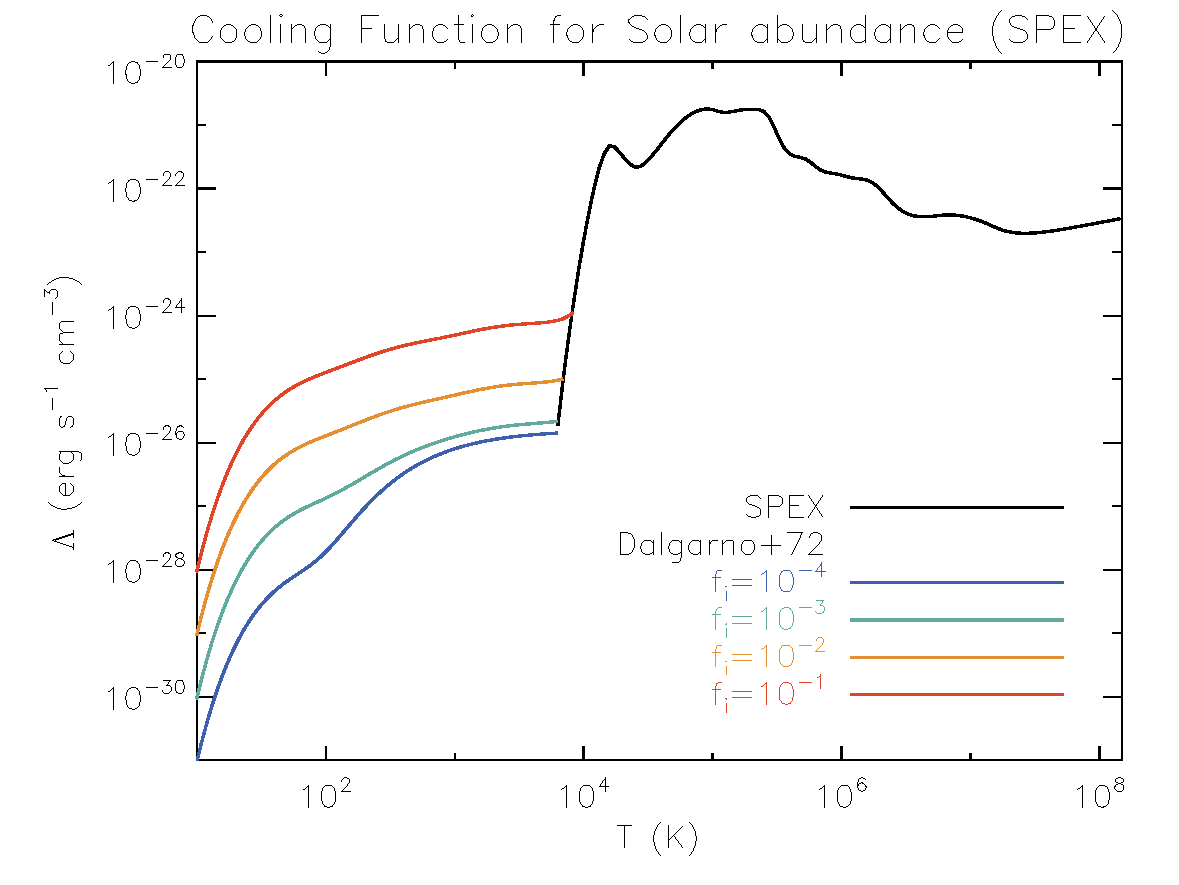
\includegraphics[width=0.5\textwidth]{ISM/spex_cool} &  
      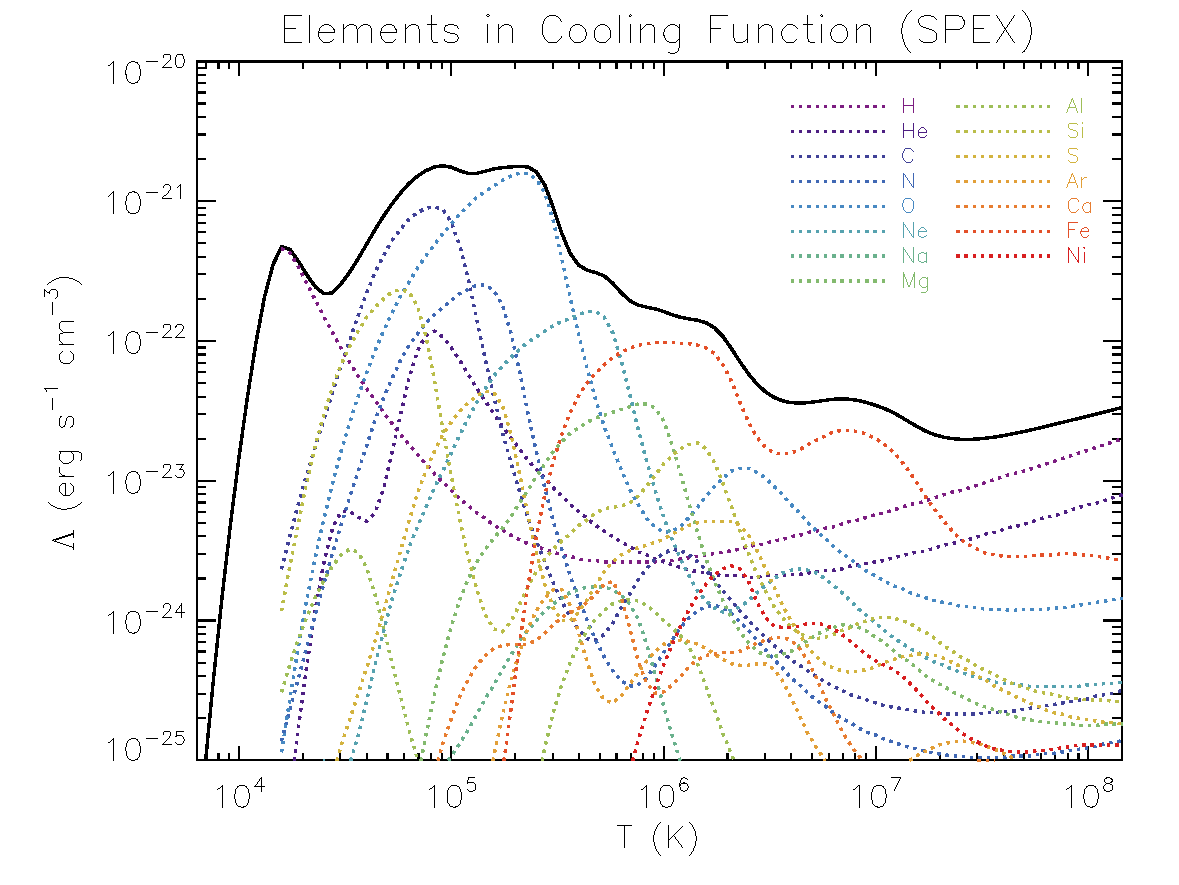
\includegraphics[width=0.5\textwidth]{ISM/spex_cool_elements}    
    \end{array}$ 
   \end{center} 
    \caption{Cooling function in Collisional Ionization Equilibrium (CIE). I made use of SPEX pacakge\cite{Schure:09}. {\it left panel}: The cooling functions in low Temperature ($T < 10^{4}$ K) are computed from \cite{Dalgarno:72}, and the colored lines represent the cooling curves in different ionization fraction ($f_{i}=n_{e}/n_{H}$). {\it right panel}: The contribution of each elements on the cooling curve.} 
   \label{fig:spexCool} 
\end{figure}

\bigskip
\section{Heating}

%\bibliographystyle{apj}
%\bibliography{citations}

   \chapter{Gravity}

\section{Gravity}
\subsection{Newtonian gravity}
A mass m' at position $\rb'$ exerts on any other mass m at position $\rb$ an attractive
force $\Fb=m {\bf g}(\rb)$; the gravitational acceleration {\bf g(r)} can be written as the 
gradient of a potential function, ${\bf g} = -\nabla \Psi$, where
\begin{equation}\label{eq:grav}
   \Psi = \frac{G m'}{|\rb - \rb'|},
\end{equation}
\begin{equation}\label{eq:gravf}
   \therefore |\nabla \Psi| = \frac{G m'}{|\rb - \rb'|^2}.
\end{equation}
Let S be a spherical surface of radius ${\rb - \rb'}$ centered at {\bf r'}, then we have
\begin{equation}
   \int_{S} \nb \cdot \nabla \Psi dS = 4 \pi G m'.
\end{equation}
It can also be verified directly that the gravitational potential of our point mass (eq 
\ref{eq:grav}) satisfies $\nabla \cdot \nabla \Psi \equiv \nabla^2 \Psi = 0$ (the Laplace equation)
everywhere except for just one point, $\rb=\rb'$. By using divergence theorem, eq \ref{eq:gravf} can 
be expressed as,
\begin{equation}\label{eq:poisson}
   \int_{V} \nabla^2 \Psi\, dV = 4 \pi G \int_{V} \rho \,dV,
\end{equation}
where V is volume inside S. Since V is arbitrary, this equation can be rewritten as a 
partial differential equation, {\bf Poisson's equation:}
\begin{equation}
   \nabla^2 \Psi = 4 \pi G \rho
\end{equation}

\bigskip
\subsection{Simple models of astrophysical fluid and their motions}
In the previous lecture we established the continuity equation (\ref{eq:continuity2}), the momentum
equation (\ref{eq:momentum}), the energy equation (\ref{eq:totE}), and Poisson's equation (\ref{eq:poisson}).
Assuming that the only body forces are due to self-gravity, so that $\fb=-\nabla \Psi$ in 
eq. \ref{eq:momentum}, these equations are:
\begin{empheq}[left=\empheqlbrack,right=\empheqrbrack]{align}
    \frac{D\rho}{Dt}+\rho\nabla\cdot\ub &= 0, \\
    \rho \frac{D \ub}{Dt} &= -\nabla P - \rho \nabla \Psi, \label{eq:mom2}\\
    \frac{DU}{Dt}-\frac{P}{\rho^2}\frac{D\rho}{Dt} &= \varepsilon - \frac{1}{\rho} \nabla \cdot \Fb,
      \label{eq:totE2} \\
    \nabla^2 \Psi &= 4 \pi G \rho. \label{eq:poisson2}
\end{empheq}
Note that these contain seven dependent variables ($\rho, P, \Psi, U$,and three components
of $\ub$).  The three equations from momentum equation, together with the rest equations,
provide six equations, and a seventh is the equation of state (\eg that for an ideal gas)
which provides a relation between any three thermodynamic state variables, so that for instance
the internal energy U and temperature T can be written in terms of P and $\rho$.($\varepsilon$
and $\Fb$ are assumed to be known functions of the other variables). Thus one might hope in
principle to solve these equations, given suitable boundary conditions. In practice this set of
equations is intractable to exact solution, and one must resort to numerical solutions. Even
these can be extremely problematic so that, for example, understanding turbulent flows is
still a very challenging research area. Moreover, an analytic solution to a somewhat idealized
problem may teach one much more than a numerical solution. One useful idealization is where we
assume that the fluid velocity and all time derivatives are zero. These are called equilibrium
solutions and describe a steady an astrophysical system evolves may be very long, so that at
any particular time the state of many astrophysical fluid bodies may be well represented by an
equilibrium model. Even when the dynamical behaviour of the body is important, it can often be
described in terms of small departures from an equilibrium state.

\bigskip
\subsection{Hydrostatic equilibrium for a self-gravitating body}

If we suppose that $\ub=0$ every where, and that all quantities are independent of time,
eq. \ref{eq:mom2} becomes
\begin{equation}\label{eq:hse}
  \nabla P + \rho \nabla \Psi = 0
\end{equation}
the continuity equation becomes trivial. A fluid satisfying eq. \ref{eq:hse} is said to
be in {\bf hydrostatic equilibrium}. If it is self-gravitating (so that $\Psi$ is determined
by the density distribution within the fluid), then eq. \ref{eq:poisson2} must also be satisfied.

Putting $\ub=0$ and $\partial/\partial t$=0, \ie $D/Dt=0$, in eq. \ref{eq:totE2}, we obtain
that the heat sources given by $\varepsilon$ must be exactly balance by the heat flux term
$\rho^{-1}\nabla \cdot \Fb$. If this holds, then the fluid is also said to be in thermal
equilibrium (See \S \ref{sec:thermaleq}).

\bigskip
\subsection{The formation of protostars}

\subsubsection{Stellar time scales}

\textbf{a) dynamical time scale}

The length of time over which changes in one part of a body can be communicated to the rest of that body.
That is also called, freefall time scale.

Assuming $|dP/dr| \ll G M_{r}\rho/r^{2}$, where $M_{r}$ is the mass of the spherical cloud,
\begin{equation}
   \frac{d^2 r}{dt^{2}} = -G \frac{M_{r}}{r^{2}} = -\frac{G}{r^{2}} \frac{4\pi}{3} \rho_{0} r_{0}^{3}, 
\end{equation}
where, $r_{0}$ and $\rho_{0}$ is the initial radius and density of the sphere. Multiplying the velocity 
of the surface  of the sphere for both sides,
\begin{equation}
   \frac{dr}{dt}\frac{d^2 r}{dt^{2}} = -\frac{G}{r^{2}} \frac{4\pi}{3} \rho_{0} r_{0}^{3} \frac{dr}{dt},
\end{equation}
which can be integrated to give
\begin{equation}
   \frac{1}{2}\left( \frac{dr}{dt} \right)^{2} = \left( \frac{4\pi}{3}G\rho_{0}r_{0}^{3} \right)\frac{1}{r} + C_{1}.
\end{equation}
where $C_{1}$ can be evaluated by, $dr/dt=0$ when $r=r_{0}$. This gives
\begin{equation}
   C_{1} = -\frac{4\pi}{3} G \rho_{0} r_{0}^2.
\end{equation}
therefore,
\begin{equation}
   \frac{dr}{dt} = - \left[ \frac{8\pi}{3}G \rho_{0} r_{0}^{2} \left( \frac{r_{0}}{r} -1 \right) \right]^{1/2}.
\end{equation}
Substituting $\theta \equiv r/r_{0}$ and $K \equiv \left( \frac{8\pi}{3} G \rho_{0} \right)^{1/2}$ gives,
\begin{equation}
   \frac{d\theta}{dt} = - K \left( \frac{1}{\theta} -1 \right)^{1/2}.
\end{equation}
Making another substitution, $\theta \equiv \cos^2{\phi}$, then
\begin{equation}
   \cos^{2}{\phi} \frac{d\phi}{dt} = \frac{K}{2}.
\end{equation}
This will be integrated to yield
\begin{equation}
   \frac{\sin{2\phi}}{4} + \frac{\phi}{2} = \frac{K}{2}t + C_{2}.
\end{equation}
where $C_{2}$ can be evaluated by, $r=r_{0}$ when $t=0$ implying $\theta=1$ or $\phi=0$ at the beginning of the collapse,
then gives $C_{2}=0$.

Consequently, the freefall time scale or dynamical time scale can be calculated by, $\theta=0$ or $\phi = \pi/2$,
\begin{eqnarray}\label{eq:fftime}
   t_{dyn} = t_{ff} &=& \frac{\pi}{2\,K} \nonumnext
                    &=& \left( \frac{3\pi}{32} \frac{1}{G \rho_{0}}\right)^{1/2}.
\end{eqnarray}

\textbf{b) thermal time scale}

The time scale on which the star would contract if its nuclear energy sources were turned off. And 
it is also called, kelvin-Helmholtz time scale:

\begin{equation}
   t_{KH} \approx \frac{G M^{2}/R_{*}}{L}.
\end{equation}

\textbf{c) nuclear time scale}
The heat released by fusing a mass $\triangle M c^{2}$. Therefore the time required to exhaust all the star's 
hydrogen is
\begin{equation}
   t_{nuc} = \frac{0.007 M c^{2}}{L}
\end{equation}

\subsubsection{Jean's Instability}\label{subsubsec:Jean}

Two methods will be described to derive Jean's Mass.

\textbf{a) From virial theorem}

The potential energy is,
\begin{equation}
   dU = G \frac{M_{interior}M_{shell}}{r}.
\end{equation}
Integrating the equation, 
\begin{equation}
   U = G \int^{0}_{R} \frac{4/3\pi r^{3}\rho ~4\pi r^{2} \rho\,dr}{r} = -\frac{3}{5} \frac{G M^{2}}{R},
\end{equation}
where $\rho = M / (\frac{4}{3}\pi R^{3})$.

The kinetic energy is
\begin{equation}
   K = N_{H}~\frac{3}{2}kT = \frac{M}{\mu m_{H}}~\frac{3}{2}kT.
\end{equation}
Using a virial theorem, 2K+U=0,
\begin{equation}
   \frac{3}{5}\frac{G M^{2}}{R} = 3 \frac{M k T}{\mu m_{H}},
\end{equation}
therefore, the Jean's mass can be calculated to
\begin{equation}
   M_{J} = \left( \frac{5 k T}{G\mu m_{H}} \right)^{3/2} \left( \frac{3}{4\pi \rho} \right)^{1/2},
\end{equation}
because $R=\left( M/(\frac{4}{3}\pi \rho) \right)^{1/3}$. The following length is
\begin{equation}
   R_{J} = \left( \frac{M_{J}}{\frac{4}{3}\pi\rho} \right)^{1/3} = \left( \frac{5 k T}{G\mu m_{H}} \right)^{1/2} \left( \frac{3}{4\pi\rho} \right)^{1/2},
\end{equation}
where the Jean's length, $\lambda_{J} = 2 R_{J}$.

\textbf{b) From freefall time}

The freefall time scale is, from Eqn. \ref{eq:fftime}, 
\begin{equation}
  t_{ff} = \left( \frac{3\pi}{32} \frac{1}{G \rho_{0}}\right)^{1/2}.
\end{equation}
In order to collapse the cloud, the freefall time scale should be less than the crossing time scale which 
is the time scale in which the information propagates from edge to edge, that is
\begin{equation}
   t_{cs} = \frac{\lambda_{J}}{Cs},
\end{equation}
where $Cs$ is the sound speed of $\sqrt{\frac{kT}{\mu m_{H}}}$. As a result,
\begin{equation}
   \left( \frac{3\pi}{32} \frac{1}{G \rho_{0}}\right)^{1/2} = \frac{\lambda_{J}}{Cs}
\end{equation}
or,
\begin{equation}
   \lambda_{J} = \left( \frac{3\pi k T}{32 G \rho \mu m_{H}} \right)^{1/2}.
\end{equation}

\bigskip
\subsection{Special relativity}
to be described

\bigskip
\subsection{General relativity}
to be described
section{Gravity}
\subsection{Newtonian gravity}
A mass m' at position $\rb'$ exerts on any other mass m at position {\bf r} an attractive
force $\Fb=m{ {\bf g}(\rb)}$; the gravitational acceleration ${\bf g}(\rb)$ can be written as the 
gradient of a potential function, ${\bf g} = -\nabla \Psi$, where
\begin{equation}\label{eq:grav}
   \Psi = \frac{G m'}{|\rb - \rb'|},
\end{equation}
\begin{equation}\label{eq:gravf}
   \therefore |\nabla \Psi| = \frac{G m'}{|\rb - \rb'|^2}.
\end{equation}
Let S be a spherical surface of radius $|\rb - \rb'|$ centered at $\rb'$, then we have
\begin{equation}
   \int_{S} \nb \cdot \nabla \Psi dS = 4 \pi G m'.
\end{equation}
It can also be verified directly that the gravitational potential of our point mass (eq 
\ref{eq:grav}) satisfies $\nabla \cdot \nabla \Psi \equiv \nabla^2 \Psi = 0$ (the Laplace equation)
everywhere except for just one point, $\rb=\rb'$. By using divergence theorem, eq \ref{eq:gravf} can 
be expressed as,
\begin{equation}\label{eq:poisson}
   \int_{V} \nabla^2 \Psi\, dV = 4 \pi G \int_{V} \rho \,dV,
\end{equation}
where V is volume inside S. Since V is arbitrary, this equation can be rewritten as a 
partial differential equation, {\bf Poisson's equation:}
\begin{equation}
   \nabla^2 \Psi = 4 \pi G \rho
\end{equation}

\bigskip
\subsection{Simple models of astrophysical fluid and their motions}
In the previous lecture we established the continuity equation (\ref{eq:continuity2}), the momentum
equation (\ref{eq:momentum}), the energy equation (\ref{eq:totE}), and Poisson's equation (\ref{eq:poisson}).
Assuming that the only body forces are due to self-gravity, so that $\fb=-\nabla \Psi$ in 
eq. \ref{eq:momentum}, these equations are:
\begin{empheq}[left=\empheqlbrack,right=\empheqrbrack]{align}
    \frac{D\rho}{Dt}+\rho\nabla\cdot\ub &= 0, \\
    \rho \frac{D \ub}{Dt} &= -\nabla P - \rho \nabla \Psi, \label{eq:mom2}\\
    \frac{DU}{Dt}-\frac{P}{\rho^2}\frac{D\rho}{Dt} &= \varepsilon - \frac{1}{\rho} \nabla \cdot \Fb,
      \label{eq:totE2} \\
    \nabla^2 \Psi &= 4 \pi G \rho. \label{eq:poisson2}
\end{empheq}
Note that these contain seven dependent variables ($\rho, P, \Psi, U$,and three components
of $\ub$).  The three equations from momentum equation, together with the rest equations,
provide six equations, and a seventh is the equation of state (\eg that for an ideal gas)
which provides a relation between any three thermodynamic state variables, so that for instance
the internal energy U and temperature T can be written in terms of P and $\rho$.($\varepsilon$
and $\Fb$ are assumed to be known functions of the other variables). Thus one might hope in
principle to solve these equations, given suitable boundary conditions. In practice this set of
equations is intractable to exact solution, and one must resort to numerical solutions. Even
these can be extremely problematic so that, for example, understanding turbulent flows is
still a very challenging research area. Moreover, an analytic solution to a somewhat idealized
problem may teach one much more than a numerical solution. One useful idealization is where we
assume that the fluid velocity and all time derivatives are zero. These are called equilibrium
solutions and describe a steady an astrophysical system evolves may be very long, so that at
any particular time the state of many astrophysical fluid bodies may be well represented by an
equilibrium model. Even when the dynamical behaviour of the body is important, it can often be
described in terms of small departures from an equilibrium state.

\bigskip
\subsection{Hydrostatic equilibrium for a self-gravitating body}

If we suppose that $\ub=0$ every where, and that all quantities are independent of time,
eq. \ref{eq:mom2} becomes
\begin{equation}\label{eq:hse}
  \nabla P + \rho \nabla \Psi = 0
\end{equation}
the continuity equation becomes trivial. A fluid satisfying eq. \ref{eq:hse} is said to
be in {\bf hydrostatic equilibrium}. If it is self-gravitating (so that $\Psi$ is determined
by the density distribution within the fluid), then eq. \ref{eq:poisson2} must also be satisfied.

Putting $\ub=0$ and $\partial/\partial t$=0, \ie D/Dt=0, in eq. \ref{eq:totE2}, we obtain
that the heat sources given by $\varepsilon$ must be exactly balance by the heat flux term
$\rho^{-1}\nabla \cdot \Fb$. If this holds, then the fluid is also said to be in thermal
equilibrium (See \S \ref{sec:thermaleq}).

\bigskip
\subsection{The formation of protostars}

\subsubsection{Stellar time scales}

\textbf{a) dynamical time scale}

The length of time over which changes in one part of a body can be communicated to the rest of that body.
That is also called, freefall time scale.

Assuming $|dP/dr| \ll G M_{r}\rho/r^{2}$, where $M_{r}$ is the mass of the spherical cloud,
\begin{equation}
   \frac{d^2 r}{dt^{2}} = -G \frac{M_{r}}{r^{2}} = -\frac{G}{r^{2}} \frac{4\pi}{3} \rho_{0} r_{0}^{3}, 
\end{equation}
where, $r_{0}$ and $\rho_{0}$ is the initial radius and density of the sphere. Multiplying the velocity 
of the surface  of the sphere for both sides,
\begin{equation}
   \frac{dr}{dt}\frac{d^2 r}{dt^{2}} = -\frac{G}{r^{2}} \frac{4\pi}{3} \rho_{0} r_{0}^{3} \frac{dr}{dt},
\end{equation}
which can be integrated to give
\begin{equation}
   \frac{1}{2}\left( \frac{dr}{dt} \right)^{2} = \left( \frac{4\pi}{3}G\rho_{0}r_{0}^{3} \right)\frac{1}{r} + C_{1}.
\end{equation}
where $C_{1}$ can be evaluated by, $dr/dt=0$ when $r=r_{0}$. This gives
\begin{equation}
   C_{1} = -\frac{4\pi}{3} G \rho_{0} r_{0}^2.
\end{equation}
therefore,
\begin{equation}
   \frac{dr}{dt} = - \left[ \frac{8\pi}{3}G \rho_{0} r_{0}^{2} \left( \frac{r_{0}}{r} -1 \right) \right]^{1/2}.
\end{equation}
Substituting $\theta \equiv r/r_{0}$ and $K \equiv \left( \frac{8\pi}{3} G \rho_{0} \right)^{1/2}$ gives,
\begin{equation}
   \frac{d\theta}{dt} = - K \left( \frac{1}{\theta} -1 \right)^{1/2}.
\end{equation}
Making another substitution, $\theta \equiv \cos^2{\phi}$, then
\begin{equation}
   \cos^{2}{\phi} \frac{d\phi}{dt} = \frac{K}{2}.
\end{equation}
This will be integrated to yield
\begin{equation}
   \frac{\sin{2\phi}}{4} + \frac{\phi}{2} = \frac{K}{2}t + C_{2}.
\end{equation}
where $C_{2}$ can be evaluated by, $r=r_{0}$ when $t=0$ implying $\theta=1$ or $\phi=0$ at the beginning of the collapse,
then gives $C_{2}=0$.

Consequently, the freefall time scale or dynamical time scale can be calculated by, $\theta=0$ or $\phi = \pi/2$,
\begin{eqnarray}\label{eq:fftime}
   t_{dyn} = t_{ff} &=& \frac{\pi}{2\,K} \nonumnext
                    &=& \left( \frac{3\pi}{32} \frac{1}{G \rho_{0}}\right)^{1/2}.
\end{eqnarray}

\textbf{b) thermal time scale}

The time scale on which the star would contract if its nuclear energy sources were turned off. And 
it is also called, kelvin-Helmholtz time scale:

\begin{equation}
   t_{KH} \approx \frac{G M^{2}/R_{*}}{L}.
\end{equation}

\textbf{c) nuclear time scale}
The heat released by fusing a mass $\triangle M c^{2}$. Therefore the time required to exhaust all the star's 
hydrogen is
\begin{equation}
   t_{nuc} = \frac{0.007 M c^{2}}{L}
\end{equation}

\subsubsection{Jean's Instability}\label{subsubsec:Jean}

Two methods will be described to derive Jean's Mass.

\textbf{a) From virial theorem}

The potential energy is,
\begin{equation}
   dU = G \frac{M_{interior}M_{shell}}{r}.
\end{equation}
Integrating the equation, 
\begin{equation}
   U = G \int^{0}_{R} \frac{4/3\pi r^{3}\rho ~4\pi r^{2} \rho\,dr}{r} = -\frac{3}{5} \frac{G M^{2}}{R},
\end{equation}
where $\rho = M / (\frac{4}{3}\pi R^{3})$.

The kinetic energy is
\begin{equation}
   K = N_{H}~\frac{3}{2}kT = \frac{M}{\mu m_{H}}~\frac{3}{2}kT.
\end{equation}
Using a virial theorem, 2K+U=0,
\begin{equation}
   \frac{3}{5}\frac{G M^{2}}{R} = 3 \frac{M k T}{\mu m_{H}},
\end{equation}
therefore, the Jean's mass can be calculated to
\begin{equation}
   M_{J} = \left( \frac{5 k T}{G\mu m_{H}} \right)^{3/2} \left( \frac{3}{4\pi \rho} \right)^{1/2},
\end{equation}
because $R=\left( M/(\frac{4}{3}\pi \rho) \right)^{1/3}$. The following length is
\begin{equation}
   R_{J} = \left( \frac{M_{J}}{\frac{4}{3}\pi\rho} \right)^{1/3} = \left( \frac{5 k T}{G\mu m_{H}} \right)^{1/2} \left( \frac{3}{4\pi\rho} \right)^{1/2},
\end{equation}
where the Jean's length, $\lambda_{J} = 2 R_{J}$.

\textbf{b) From freefall time}

The freefall time scale is, from Eqn. \ref{eq:fftime}, 
\begin{equation}
  t_{ff} = \left( \frac{3\pi}{32} \frac{1}{G \rho_{0}}\right)^{1/2}.
\end{equation}
In order to collapse the cloud, the freefall time scale should be less than the crossing time scale which 
is the time scale in which the information propagates from edge to edge, that is
\begin{equation}
   t_{cs} = \frac{\lambda_{J}}{Cs},
\end{equation}
where $Cs$ is the sound speed of $\sqrt{\frac{kT}{\mu m_{H}}}$. As a result,
\begin{equation}
   \left( \frac{3\pi}{32} \frac{1}{G \rho_{0}}\right)^{1/2} = \frac{\lambda_{J}}{Cs}
\end{equation}
or,
\begin{equation}
   \lambda_{J} = \left( \frac{3\pi k T}{32 G \rho \mu m_{H}} \right)^{1/2}.
\end{equation}

\bigskip
\subsection{Special relativity}
to be described

\bigskip
\subsection{General relativity}
to be described

%\bibliographystyle{apj}
%\bibliography{citations}

   \chapter{Galactic Dynamics}

\section{Galactic Dynamics}

\bigskip
\subsection{Stellar distribution}\label{subsec:stardist}

The surface brightness (stellar components) of elliptical galaxy falls off smoothly with radius,
and it can be fitted by some empirical profiles:

\noi{\bf 1) S\'{e}rsic profile}

\begin{equation}\label{eq:Sersic}
    I(r) = I_{e}\,\exp{ \left\{ -\nu_{n} \left[ \left( \frac{r}{r_{e}}\right)^{1/n} - 1 \right] \right\}},
\end{equation}
where, $r_{e}$ is effective radius, the radius of the isophote containing half of the total luminosity.

\medskip
\noi{\bf 2) De Vaucouleurs profile} 

When $n=4,\,\nu_{4}=7.66925$, the S\'{e}rsic profile [eq.~(\ref{eq:Sersic})] becomes de Vaucouleurs profile,
\begin{equation}
    I(r) = I_{e}\,\exp{ \left\{ -\nu_{4} \left[ \left( \frac{r}{r_{e}}\right)^{1/4} - 1 \right] \right\}}.
\end{equation}


\medskip
\noi{\bf 3) King profile}

King profile was developed from the singular isothermal sphere model, at which the distribution function 
follows the balance between the gravitational potential and velocity dispersion (analogue to the hydrostatic 
equilibrium sphere with adiabatic index of $\gamma=1$).
\begin{equation}
    I(r) = K\,\left\{ \left[ 1 + \left( \frac{r}{r_{c}} \right)^{2} \right]^{-1/2} 
            - \left[ 1+ \left( \frac{r_{t}}{r} \right)^{2} \right]^{-1/2} \right\}^{2},
\end{equation}
where $r_{c}$ is the core radius $\left[ \frac{I(r=0)}{I(r=r_{c})}=2 \right]$, $r_{t}$ is the tidal radius where 
is considered as outermost limit of the system by observers, and $K$ is the scale factor.

This profile gives a very good representation of star counts in tidally-limited globular clusters and low-density
spheroidal galaxies.

\medskip
\noi{\bf 4) Exponential profile}

Disks of spiral galaxies are known to show profiles described well by the exponential law:
\begin{equation}
    I(r) = I_{0}\,\exp{\left( -\frac{r}{h} \right)},
\end{equation}
where $h$ is the exponential scale length.

\bigskip
\subsection{Dark matter profile: Two-power density models \cite{Binney:87}}

Numerical simulations of the clustering of dsrk matter particles suggest that the mass density with dark halo 
has a similar structure. Mostly, the two-power density models has been applied:
\begin{equation}\label{eq:twoden_dm}
    \rho(r) = \frac{\rho_{0}}{(r/a)^{\alpha}(1+r/a)^{\beta-\alpha}}.
\end{equation}
According to the sets of $(\alpha,\beta)$, the model can be classified with Jaffe, Hernquist, and NFW profiles. 
The mass interior to radidus $r$ is
\begin{equation}\label{eq:twoden_M}
    M(r) = 4\pi\rho_{0}\,a^{3} \int^{r/a}_{0} ds\,\frac{s^{2-\alpha}}{(1+s)^{\beta-\alpha}}.
\end{equation}

\medskip
\noi{\bf 1) Jaffe profile}

$\alpha=2$ and $\beta=4$ in eq.~(\ref{eq:twoden_dm}).
Therefore, from eq.~(\ref{eq:twoden_M}), the mass profile becomes
\begin{equation}
    M(r) = 4\pi\rho_{0}\,a^{3} \frac{r/a}{1+r/a},
\end{equation}
and the potential becomes
\begin{eqnarray}
    \Phi(r) &=& -G\int^{\infty}_{r} dr\,\frac{M(r)}{r^{2}} \nonumnext
            &=& -4\pi\rho_{0}\,a^{2}\, \ln{(1+a/r)}.
\end{eqnarray}

\noi{\bf 2) Hernquist profile}

$\alpha=1$ and $\beta=4$ in eq.~(\ref{eq:twoden_dm}).
Therefore, from eq.~(\ref{eq:twoden_M}), the mass profile becomes
\begin{equation}
    M(r) = 4\pi\rho_{0}\,a^{3} \frac{(r/a)^{2}}{2(1+r/a)^{2}},
\end{equation}
and the potential becomes
\begin{eqnarray}
    \Phi(r) &=& -G\int^{\infty}_{r} dr\,\frac{M(r)}{r^{2}} \nonumnext
            &=& -4\pi\rho_{0}\,a^{2}\, \frac{1}{2(1+r/a)}.
\end{eqnarray}


\noi{\bf 3) NFW profile}

NFW profile is named from Navarro, Frenk, \& White (1995).
$\alpha=1$ and $\beta=3$ in eq.~(\ref{eq:twoden_dm}).
Therefore, from eq.~(\ref{eq:twoden_M}), the mass profile becomes
\begin{equation}
    M(r) = 4\pi\rho_{0}\,a^{3} \left[ \ln{(1+r/a)} - \frac{r/a}{1+r/a} \right],
\end{equation}
and the potential becomes
\begin{eqnarray}
    \Phi(r) &=& -G\int^{\infty}_{r} dr\,\frac{M(r)}{r^{2}} \nonumnext
            &=& -4\pi\rho_{0}\,a^{2}\, \frac{\ln{(1+r/a)}}{r/a}.
\end{eqnarray}


\bigskip
\subsection{Fundamental Plane}
Fundamental plane is an empirical relationship of observed elliptical galaxies between the
effective radius $r_{e}$ (see \S\ref{subsec:stardist}), average surface brightness $I$ (or
Luminosity $L_{\rm B}$), and central velocity dispersion $\sigma_{0}$ (Fig.~\ref{fig:fundp}).
\begin{equation}
    \log{r_{e}} = A\,\log{\sigma_{0}} + B\,\log{L_{\rm B}} + C.
\end{equation}

\begin{figure}[!htbp]
    \centering
    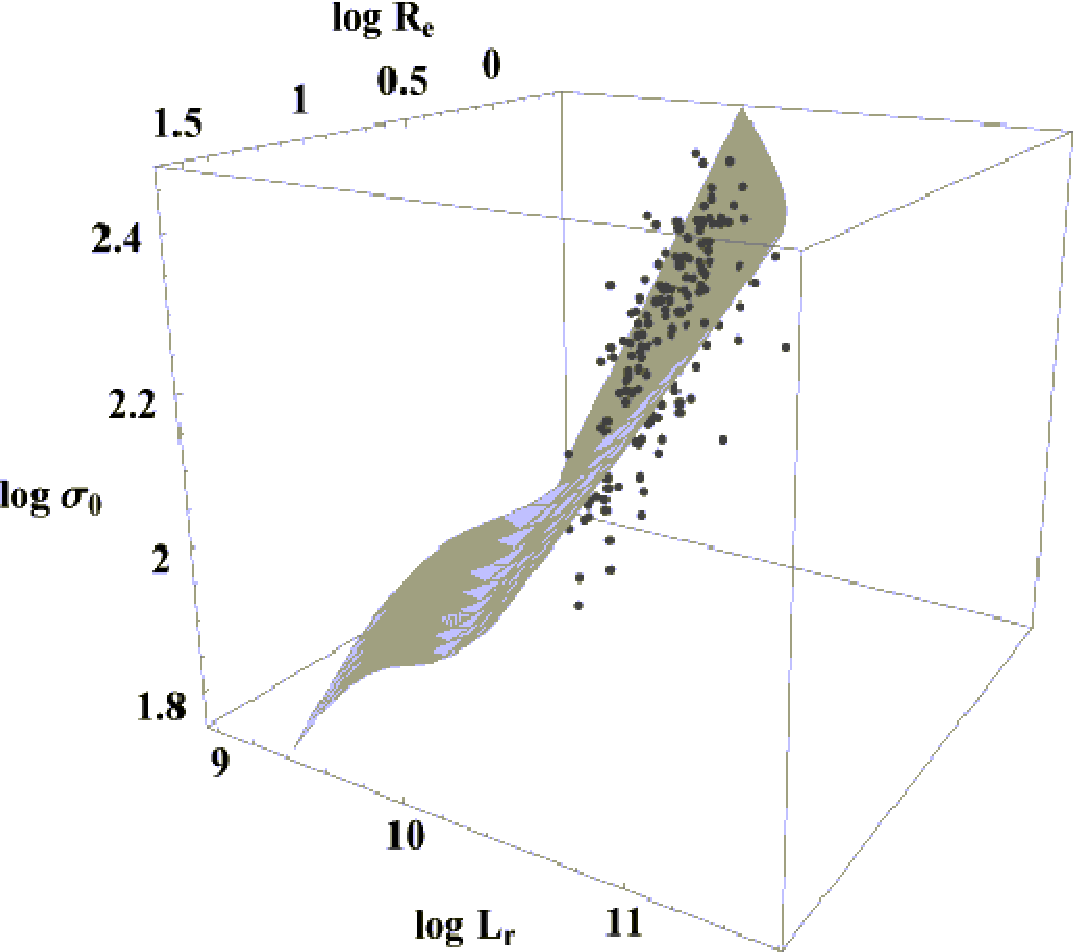
\includegraphics[width=0.7\textwidth]{Galactic/fundamentalplane}
    \caption{3 dimensional space ($r_{e},\,\sigma_{0},\,L$) of Fundamental Plane}
    \label{fig:fundp}
\end{figure}

\bigskip
\subsection{Faber-Jackson relation}
This relation is an empirical power-law relation between the luminosity $L$ and the central 
stellar velocity dispersion $\sigma_{0}$ of elliptical galaxies. 

The theoretical derivation requires some assumptions:

The gravitational potential for uniform sphere (constant density; see \S\ref{subsec:potunisp}) is 
\begin{equation}
    U = -\frac{3}{5} \frac{G\,M}{R}.
\end{equation}
And the kinetic energy is 
\begin{equation}
    K = \frac{3}{2} M\,\sigma_{0}^{2},
\end{equation}
where $\sigma_{0}$ is 1-dimensional velocity dispersion ($3\sigma_{0}^{2} = V^{2}$ where $V$
is total velocity dispersion). From the virial therom ($2K+U=0$), it follows
\begin{equation}
    \sigma^{2}=\frac{1}{5}\frac{G\,M}{R}.
\end{equation}
Assuming the constant mass to light ratio $\Upsilon=M/L$, then 
\begin{equation}
    R = \frac{1}{5}\frac{\Upsilon L\,G}{R}.
\end{equation}
If we assume that the surface brightness $I=L/(4\pi R^{2})$ is constant (highly unlikely),
then
\begin{equation}
    L = \frac{25\,\sigma^{4}}{4\pi\,G^{2}\,I\,\Upsilon^{2}} \propto \sigma^{4}.
\end{equation}
Since the assumptions during the derivation are poor, the empirical power varies between 3 (less massive galaxies) 
and 15 (more massive galaxies).

\bigskip
\subsection{Tully-Fisher relation}
The rotation rate of spiral galaxies in the flat part of the circular-speed curve is
related to their luminosity.

\bigskip
\subsection{Nearly circular orbits: Epicycle frequency}
In disk galaxies, many stars are on nearly circular orbits. We define
\begin{equation}
   x \equiv r - r_{g},
\end{equation}
where $r_{g}$ is the guiding center radius for an orbit.
The effective potential is 
\begin{equation}
   \Phi_{\rm eff} = \Phi + \frac{l^{2}}{2\,r^{2}},
\end{equation}
where $l$ is a specific angular momentum $l = r\,v_{\phi}$, and $v_{\phi}$ is rotation velocity.
Expanding $\Phi_{\rm eff}$ in a Taylor series results in
\begin{equation}\label{eq:PhieTyl}
    \Phi_{\rm eff} (r) = \Phi_{\rm eff}(r_{g}) + \left. \frac{\partial \Phi_{\rm eff}}{\partial r} \right|_{r=r_{g}} x
                    + \frac{1}{2} \left. \frac{\partial^{2} \Phi_{\rm eff}}{\partial r^{2}} \right|_{r=r_{g}} x^{2} + O(x^{2}).
\end{equation}
The first order term (second term in RHS) vanishes because $\Phi_{\rm eff}$ is assumed to be symmetic about $r=r_{g}$.
So the eq.~(\ref{eq:PhieTyl}) can be approximated to 
\begin{equation}
    \Phi_{\rm eff} (r) \simeq \Phi_{\rm eff}(r_{g}) 
                    + \frac{1}{2} \left. \frac{\partial^{2} \Phi_{\rm eff}}{\partial r^{2}} \right|_{r=r_{g}} x^{2} 
\end{equation}
The equation of motion is
\begin{eqnarray}
    \ddot{x} = -\frac{\Phi_{\rm eff}}{x} &=& - \left. \frac{\partial^{2} \Phi_{\rm eff}}{\partial r^{2}} \right|_{r=r_{g}} x \\
             &=& -\kappa^{2}\,x,
\end{eqnarray}
where $\kappa$ is called \emph{epicycle frequency}.
\begin{equation}\label{eq:epi1}
    \kappa^{2}(r_{g}) = \left. \frac{\partial^{2} \Phi_{\rm eff}}{\partial r^{2}} \right|_{r=r_{g}}
             = \left. \frac{\partial^{2} \Phi}{\partial r^{2}} \right|_{r=r_{g}} + \frac{3\,l^{2}}{r_{g}^{4}}.
\end{equation}
Since the circular frequency is related with the gravitational force,
\begin{equation}
    \frac{\partial \Phi}{\partial r} = r\, \Omega^{2},
\end{equation}
where $\Omega = l/r^{2}$ is an angular frequency of the circular orbit. Plugging into eq.~(\ref{eq:epi1}) gives
\begin{eqnarray}\label{eq:epi2}
    \kappa^{2}(r_{g}) &=& \left( r \frac{d\,\Omega^{2}}{d\,r} + 4\,\Omega^{2} \right)_{r=r_{g}} \\
                      &=& \left[ \frac{1}{r^{3}} \frac{d}{d\,r} \left( r^{4}\,\Omega^{2} \right) \right]_{r=r_{g}}.
\end{eqnarray}
If we assumes that the angular frequency has a power-law relationship with the radius ($\Omega \sim r^{q}$),
the eq.~(\ref{eq:epi2}) can be expressed as
\begin{equation}
    \kappa^{2} = (4 + 2q)\,r^{2q} = (4 + 2q)\,\Omega^{2}.
\end{equation}
Note the several examples of the epicycle frequency:
\begin{empheq}[left=\empheqlbrace]{align}
    {\rm Rigid~ rotation} &:      \Omega \sim R^{0} \rightarrow \kappa^{2} = 4\Omega^{2} \\
    {\rm Keplerian~ rotation} &:  \Omega \sim R^{-3/2} \rightarrow \kappa^{2} = \Omega^{2} \\
    {\rm Flat~ rotation} &:       \Omega \sim R^{-1} \rightarrow \kappa^{2} = 2\Omega^{2} 
\end{empheq}
In the rigid and Keplerian rotations, the epicycle motion is closed, but in the flat rotation 
it is not closed.

\bigskip
\subsection{Luminosity function: Schechter law}
The luminosity function $\phi(L)$ describes the relative numbers of galaxies of different luminosities,
and is defined so that $\phi(L)\,dL$ is the number of galaxies in the luminosity interal $L \rightarrow L+dL$
in a representative unit volume of the universe. The analytic approximation is know as Schechter law:
\begin{equation}
    \phi(L)\,dL = \phi_{\star} \left( \frac{L}{L_{\star}} \right)^{\alpha} \exp{\left(-\frac{L}{L_{\star}}\right)}\frac{dL}{L},
\end{equation}
where $\phi_{\star} \simeq 4.9\times10^{-3}\,{\rm Mpc^{-3}},\,\alpha=-1.1,\,{\rm and}\, L_{\star}\simeq 2.9\times10^{10}\,L_{\odot}$
in the $R$ band.

\bigskip
\subsection{Star Formation Rate: Kennicutt-Schmidt Law}
Kennicutt-Schmidt law is the empirical relationship between the global star formation in a galaxy 
and $\Sigma_{\rm gas,disk}$ the gas surface density averaged over the ``optical disk'' of the galaxy, finding
that the star formation rate per unit area $\Sigma_{\rm SFR,disk}$ varies approximately as
\begin{eqnarray}
    \Sigma_{\rm SFR,disk} &=& (2.5\pm0.7)\times 10^{-4} \left( \frac{\Sigma_{\rm gas,disk}}{M_{\odot}{\rm pc^{-2}}} \right)^{1.4\pm 0.15}\,M_{\odot}\,{\rm kpc^{-2}{yr^{-1}}} \\
                          &\propto& \Sigma_{\rm gas,disk}^{1.4}.
\end{eqnarray}

\bigskip
\subsection{Initial Mass Function (IMF): Salpeter or Kroupa}
According to single burst stellar population synthesis models, most of the stellar mass is lost 
at early times, before an age of $\sim 2$ Gyr: 25\% and 36\% of the total initial mass are lost
for the Salpeter and Kroupa IMF, respectively. The approxmiated model\cite{Kim:13} is:
\begin{equation}
    \dot{M}_{\star}(t) = 10^{-12}\,A\times \left( \frac{M_{\star}}{M_{\odot}} \right) t_{12}^{-1.3}~~~M_{\odot}{\rm yr^{-1}},
\end{equation}
where $M_{\star}$ is the galactic stellar mass at an age of 12 Gyr, $t_{12}$ is the age in units of 12 Gyrs,
and $A=2.0~{\rm or}~3.3$ for a Salpeter or Kroupa IMF.

   \chapter{High Energy AstroPhysics}

\section{High Energy AstroPhysics}

\subsection{Schwarzschild radius}
\begin{equation}
   R_{s} = \frac{2GM}{c^{2}} 
\end{equation}

\bigskip
\subsection{Eddington limits}

For gas accretion - there is a maximum luminosity at which the environment of a black hole
of $M_{BH}$ may shine and still accrete gas, called Eddington limit, $L_{Edd}$.
This limit is obtained by setting the outward continuum radiation pressure equal to the inward
gravitational force. Denoting the gravitational potential with $\Phi$, pressure with $P$, density 
with $\rho$,
\begin{equation}
   \nabla\Phi = -\frac{\nabla P}{\rho}=\frac{\kappa}{c}F_{rad},
\end{equation}
where in the last equality we assumed that the pressure is dominated by radiation pressure
which is associated to a radiation flux, $F_{rad}$. Here $\kappa$ is the opacity. There are two
primary sources of opacity for the typical densities and temperatures here:
Thomson electron scattering and bremsstrahlung (i.e labeled free-free absorption) with
\begin{equation}
    \kappa_{es}=\frac{\sigma_{T}}{m_{p}} = 0.4 ~ {\rm cm^{2}g^{-1}},
\end{equation}
\begin{equation}
    \kappa_{ff}\approx 8\times10^{22} ~{\rm cm^{2}g^{-1}} \left(\frac{\rho}{\unitd}\right) \left( \frac{T}{{\rm K}} \right)^{-7/2},
\end{equation}
where we assumed a pure hydrogen plasma for simplicity, where $m_{p}$ denotes proton mass and $\sigma_{\rm T}$ denotes the 
Thomson cross section. For the definition of the luminosity,
\begin{equation} 
   L = \int_{S} F_{rad}\cdot dS = \frac{c}{\kappa} \int_{S} \nabla\cdot dS
\end{equation}
Using Gauss's theorem,  Poisson's equation $\nabla^{2}\Phi=4\pi G \rho$, and the definition of the mass,
\begin{equation}
   L_{Edd} = \frac{c}{\kappa}\int_{V}\nabla^{2}\Phi dV = \frac{4\pi G c}{\kappa}\int_{V}\rho dV=\frac{4\pi G M c}{\kappa} 
           = 1.3\times10^{44} \left( \frac{M_{BH}}{10^{6} M_{\odot}} \right) \unitpower
\end{equation}

\bigskip
\subsection{SuperNova explosion \& Remnant}

\subsubsection{SNR phases}

There are 4 phases in the evolution of supernova remnants (SNRs): free-expansion, Sedov expansion, snowplow phase and relaxing phase.
Fig.~(\ref{fig:SNRphase}) shows the correlation between the size of bubble and the evolution time along the phases.

\begin{figure}[!htbp]
    \centering
    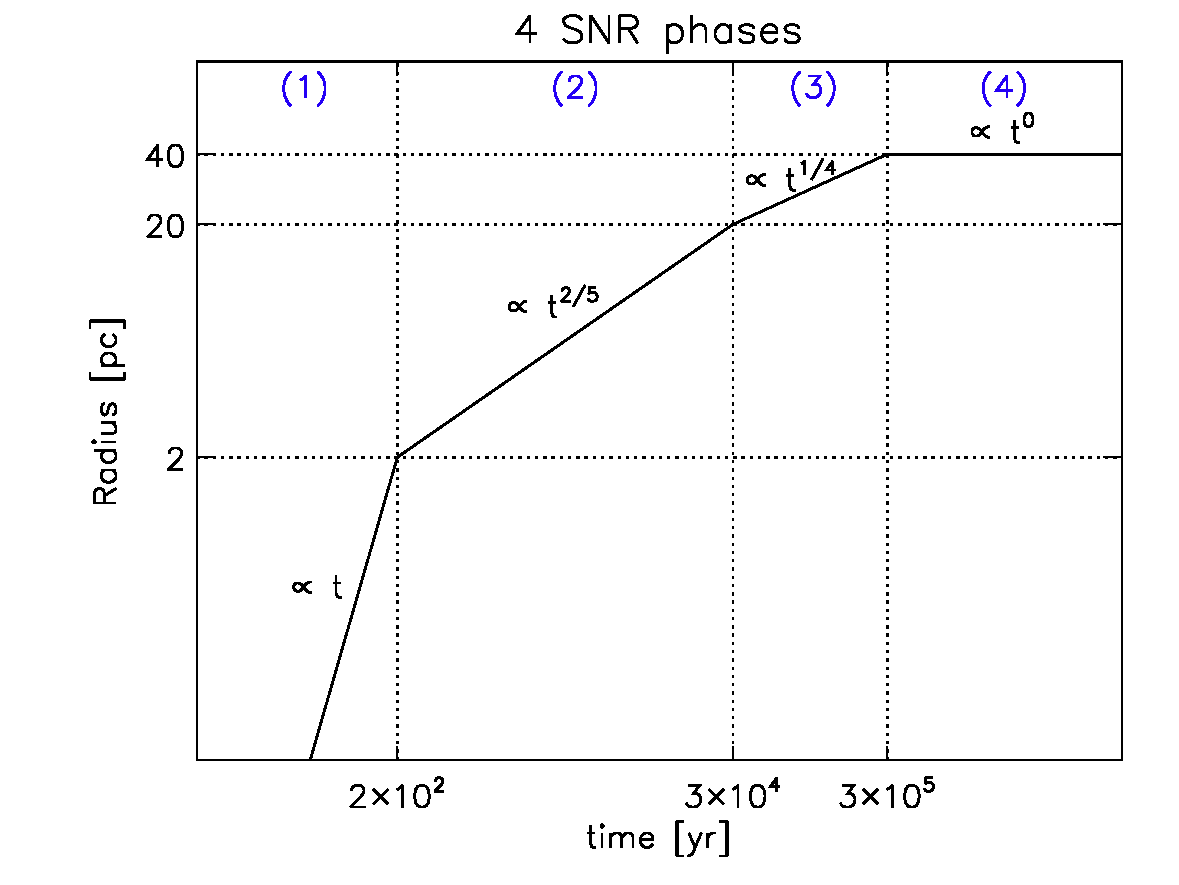
\includegraphics[width=0.7\textwidth]{HighEnergy/SNRphase}
    \caption{4 Supernova remnants phases: (1) free expansion (2) Sedov-Taylor expansion (3) Snowplow phase (4) relaxing phase.
            Note that x\&y axes are in logarithmic scale.}
    \label{fig:SNRphase}
\end{figure}

\noi (1) free expansion ($v=v_{\rm ej}=$constant)

The energy of supernova explosion is roughly:
\begin{equation}
    E_{\rm SN} \sim \frac{1}{2}\,M_{\rm ej}\,v_{\rm ej}^{2},
\end{equation}
where the ejected outflow velocity is,
\begin{equation}
    v_{\rm ej} \sim 10^{4}\, km/s \, \left( \frac{E_{\rm SN}}{10^{51}\,erg} \right)^{1/2} \left( \frac{M_{\rm ej}}{M_{\odot}} \right)^{-1/2}.
\end{equation}
The mass of swept-up gas becomes
\begin{equation}
    M_{\rm swept-up} \sim \frac{4\pi}{3}\,r^{3}\,\rho_{\rm ISM}.
\end{equation}
As a result, the bubble radius during this phase increases until $M_{\rm swept-up} \sim M_{\rm ej}$,
\begin{equation}
    r \sim 2\,pc\,\left( \frac{M_{\rm ej}}{M_{\odot}} \right)^{1/3} \left( \frac{\rho_{\rm ISM}}{10^{-24}\,g\,cm^{-3}} \right)^{-1/3},
\end{equation}
and the final time of this stage is
\begin{equation}
    t \sim \frac{r}{v_{\rm ej}} \sim 200\, yr\, \left( \frac{E_{\rm SN}}{10^{51}\,erg} \right)^{-1/2} \left( \frac{M_{\rm ej}}{M_{\odot}} \right)^{5/6}
                                 \left( \frac{\rho_{\rm ISM}}{10^{-24}\,g\,cm^{-3}} \right)^{-1/3}.
\end{equation}

\noi (2) Sedov-Taylor expansion ($E=E_{\rm SN}=$constant)

The energy is conserved in this stage: $E_{\rm SN} \propto M\,v^{2} \propto \rho_{\rm ISM}\,r^{3}\,\dot{r}^{2}$,
thereby
\begin{eqnarray}
    r^{3}\left( \frac{dr}{dt} \right)^{2} &\propto& \frac{E_{\rm SN}}{\rho_{\rm ISM}} \nonumnext
    r^{3/2}\,dr &\propto& \left( \frac{E_{\rm SN}}{\rho_{\rm ISM}} \right)^{1/2}\,dt \nonumnext
    \therefore r &\propto& \left( \frac{E_{\rm SN}}{\rho_{\rm ISM}} \right)^{1/5}\, t^{2/5} 
\end{eqnarray}

The typical outflow velocity is $\sim 200\, km/s$ and the temperature drops to $10^{6}\, K$, which emits
strong X-ray thermal bremsstrahlung.

\noi (3) Snowplow phase ($p$=constant)

The temperature drops below $10^{6}\, K$ so that radiative cooling becomes dominant by some recombination processes.
In this stage, the cold dense shell is driven by the hot interior. 
\begin{equation}
    \frac{d}{dt}(M\,v) = \frac{d}{dt}\left( \frac{4\pi}{3}\,\rho\,r^{3}\,\dot{r} \right) = 0.
\end{equation}
Assuming a thin shell forms at $t_{0}$ with the size of $r_{0}$ and the outflow velocity of $v_{0}$,
\begin{eqnarray}
    r^{3}\,\dot{r} &=& r_{0}^{3}\,v_{0} \nonumnext
    r &=& r_{0} \left[ 1 + \frac{4\,v_{0} (t-t_{0})}{r_{0}} \right]^{1/4}.
\end{eqnarray}

\noi (4) mixing phase with ISM ($r$=constant)

The typical temperature and outflow velocity are $10^{4}\, K$ and $10\, km/s$, respectively. 
The speed of ejecta becomes comparable to the sound speed of ISM.


\subsubsection{bubble with continuous energy injection:\\ (bubble at pulsars or microquasars)}

The solution for the expanding shock front supported by spin-down energy from central pulsar
wind must be a scale-free or self-similar solution, which can be expressed of the dimensionless
variable, $\eta$, where

\begin{equation}
   \eta \equiv r\,t^{l}\,\rho_{0}^{m}\,\dot{E_{0}}^{n},
\end{equation}

\noi the exponents $l$,$m$, and $n$ are determined by the requirement that $\eta$ is
dimensionless.  Since the $\dot{E_{0}}$ has the dimensionality $M\,L^{2}\,T^{-3}$, and the
$\rho_{0}$ has the dimensionality $M\,L^{-3}$, the dimensionality of $\eta$ should be
$L^{1-3m+2n}\,T^{l-3n}\,M^{m+n}$. Therefore, the exponents $l=-3/5, m=1/5,$ and $n=-1/5$,

\begin{equation}
   \eta = r \, \left( \frac{\rho_{0}}{\dot{E_{0}}t^{3}} \right)^{1/5},
\end{equation}

\noi or,

\begin{equation}\label{eq:Rs}
   R_{s}(t) = \eta \left( \frac{\dot{E_{0}}}{\rho_{0}} \right)^{1/5}\,t^{3/5}.
\end{equation}

In order to calculate the normalized factor, $\eta$, descriptions in \cite{Castor:75}
are adopted. In their notation, region b indicates a hot, almost isobaric region consisting 
of shocked stellar wind, and region c indicates a thin, dense, cold shell at radius,$R_{s}$
expending at velocity $\dot{R_{s}}$, and containing most of the swept-up ISM gas.

The dominant energy loss of region b is work against the dense shell, region c, so that the
total energy of region b should be

\begin{equation}\label{eq:Castor1}
   \dot{E_{b}} = \dot{E_{0}} - 4 \pi R_{s}^2 P_{b} \dot{R_{s}},
\end{equation}

\noi with

\begin{equation}\label{eq:Castor2}
   \frac{4}{3} \pi R_{s}^3 P_{b} = \frac{2}{3} E_{b}.
\end{equation}

In addition, the motion of the shell, region c, follows from 

\begin{equation}\label{eq:Castor3}
   \frac{d}{dt} \left[ M_{c}(t) \dot{R_{s}}(t) \right] = 4 \pi R_{s}^{2} P_{b},
\end{equation}

\noi where

\begin{equation}\label{eq:Castor4}
   M_{c}(t) = \frac{4}{3}\pi \rho_{0} R_{s}^3,
\end{equation}

\noi assuming that most of the swept-up interstellar mass remains in the shell. Combining eq. 
(\ref{eq:Castor1})-(\ref{eq:Castor4}) allows us to derive the radial evolution of the shell.
As we differentiate eq. (\ref{eq:Castor2}),

\begin{equation}
   \dot{E_{b}} = 6 \pi R_{s}^{2} \dot{R_{s}} P_{b} + 2 \pi R_{s}^3 \dot{P_{b}},
\end{equation}

\noi and combine it with eq. (\ref{eq:Castor1}),

\begin{equation}\label{eq:Castor1-1}
  \therefore \, 10 \pi R_{s}^{2} \dot{R_{s}} P_{b} + 2 \pi R_{s}^{3} \dot{P_{b}} = \dot{E_{0}}
\end{equation}

Meanwhile, eq. (\ref{eq:Castor3})\&(\ref{eq:Castor4}) can be further calculated as, 

\begin{eqnarray}\label{eq:Castor4-1}
   \frac{d}{dt} \left[ \frac{4}{3}\pi R_{s}^3 \rho_{0} \dot{R_{s}} \right] &=& 4 \pi R_{s}^2 P_{b} \nonumnext
   \rightarrow \, 3 \dot{R_{s}^2} + R_{s} \ddot{R_{s}} &=& 3 \frac{P_{b}}{\rho_{0}}.
\end{eqnarray}

For the purpose of simplification, we substitute $\eta \left( \frac{\dot{E_{0}}}{\rho_{0}}
\right)^{1/5} \equiv A$, where $A$ is constant, then we set eq. (\ref{eq:Rs}) to $R_{s}(t) =
A \, t^{3/5}$. Plugging it into eq. (\ref{eq:Castor4-1}) allows us to express $P_{b}$ as,

\begin{equation}\label{eq:Pb}
   P_{b} (t) = \frac{7}{25} A^{2} \, \rho_{0} \, t^{-4/5},
\end{equation}

Finally we plug eq. (\ref{eq:Pb}) into eq.(\ref{eq:Castor1-1}), we get

\begin{eqnarray}
   \frac{154}{125} \pi A^{5} \rho_{0} &=& \dot{E_{0}}  \nonumnext
   \therefore \, A &=& \left( \frac{\dot{E}}{\rho_{0}} \right)^{1/5} \left( \frac{125}{154 \pi} \right)^{1/5}
\end{eqnarray}

\noi or equivalently,

\begin{equation}\label{eq:eta}
   \eta = \left( \frac{125}{154 \pi} \right)^{1/5}.
\end{equation}

\bigskip
\subsection{Accretion Disk}
\subsubsection{overview}
In the 1960s, X-ray observations and radio imaging of cosmic sources led to the realization 
that compact objects are a) numerous and b) extremely bright and c) extremely luminous. Understanding
what powers these sources required the formulation of a theory of accretion.

Beyond  high energy astrophysics, accretion is important in many other scenarios, such as star formation
and growth of starcluster.

\begin{itemize}
\item Arguments for accretion onto compact objects:\\
Consider a cosmic X-ray source (either an X-ray binary or an AGN).

\subitem AGN: Observe $L_{bol}\approx 10^{45}-10^{46} ~\unitpower$ \\
     $~~~~~~~~~~~~~~~$Observe variability with $\Delta \tau \sim \rm\,hours - years$
\subitem XRB: Observe $L_{bol}\approx 10^{38} ~\unitpower$ \\
     $~~~~~~~~~~~~~~~$Observe variability with $\Delta \tau \sim 10^{-3} - 1 \rm\,sec$

\item Causality: For a stationary object emitting with considerable variability on timescale
$\Delta \tau$ (with $\ge$ 50 \% $\Delta L$), we infer a size unit of
\begin{equation}
   R_{obj} \le \Delta \tau \cdot c,
\end{equation}
from causality arguments (significant portion of the object must light up within $\Delta \tau$, and light
travel time across object must, therefore, be $\le \Delta \tau$)

$\Rightarrow \rm\,R_{AGN} \le$ AU to PC

$~~~~\rm\,R_{XRB} \le \, 100\,km\, to~ R_{\odot}$

\item Efficiency: Suppose the object is powered by consuming some fuel at some rate $\dot{M}$ and converting to radiation 
with some efficiency $\eta$:

\begin{equation}
   L = \eta \dot{M} c^{2},
\end{equation}
so,
\begin{eqnarray}
   \dot{M} = \frac{L}{\eta c^{2}} &=& 1.4\times10^{18}\,\unitmflux \left( \frac{L}{10^{38}\,\unitpower} \right) \left( \frac{10\%}{\eta} \right) \nonumnext
                                  &\cong& 2\times10^{-8} \,\unitmfluxsol \left( \frac{L}{10^{38}\, \unitpower} \right) \left( \frac{10\%}{\eta} \right)
\end{eqnarray}

\item Characteristic masses: Dynamical mass estimates are available for both AGN and XRBs

\[ \left. 
\begin{array}{rl}
M_{AGN} & \sim 10^{6} - 10^{10} \, M_{\odot}  \\ 
M_{XRB} & \sim 1 - 30 \, M_{\odot}  
\end{array}
\right\} ~ \textrm{\bf Compact Object !}  \]

\item Possible power sources:

\subitem a) Chemical: $\eta_{chem} \approx \rm eV/nucleon \approx 10^{-9}$
\subitem b) Nuclear: $\eta_{nuc} \approx \rm MeV/nucleon \approx 10^{-3}$
\subitem c) accretion:
\begin{eqnarray}
 R_{isco} &=& \frac{6GM}{c^{2}} \nonumnext
 \Delta{E_{isco}} &=& \frac{1}{2} \frac{GM m_{p}}{R_{isco}}=\frac{GM m_{p} c^{2}}{12 GM} = \frac{m_{p}c^{2}}{12} \nonumnext
 \rightarrow \eta_{acc} &\approx& \frac{1}{12} \approx 10\,\% \approx 100\times \eta_{nuc} \approx 10^{8} \eta_{chem} \nonumber
\end{eqnarray}
$~~~~~~~~$ accretion by far the most efficient power source.

\item Growth time: 
\begin{equation}
   T_{\dot{M}} = \frac{M}{\dot{M}} = 4 \times 10^{7}\, yrs \left(\frac{\eta}{10\%}\right) \left(\frac{M}{M_{\odot}}\right) \left(\frac{10^{38}\,erg\,s^{-1}}{L} \right)
\end{equation}

This immediately rules out chemical power and even a nuclear powered source with quickly run
out of fuel. We will formalize this argument further in the context of AGN.  

\end{itemize}

\subsubsection{How does accretion work?}

\textbf{Spherical/Bondi-Hoyle accretion}:  \\
Consider massive, gravitating compact object placed in a stationary, uniform medium 

$\Rightarrow$ no pressure gradients to support against gravity.

$\Rightarrow$ spherically symmetric infall (no preferred direction)

\begin{figure}[!htbp]
   \centering
   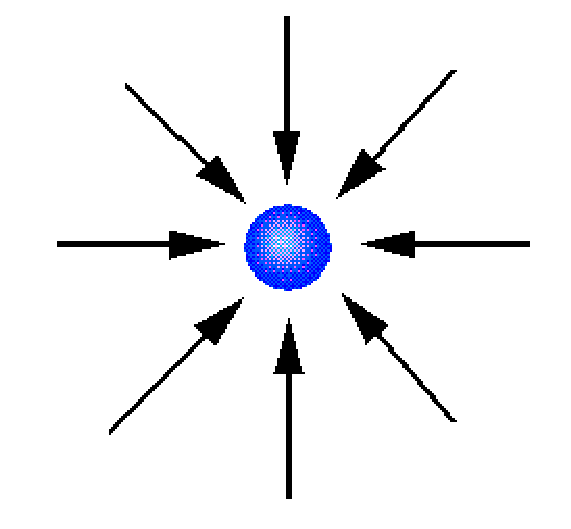
\includegraphics[width=0.25\textwidth]{HighEnergy/infall}
   \caption{sketch of spherical infall}
\label{fig:infall}
\end{figure}

Questions:

\begin{itemize}
   \item What is the structure of such a flow?
   \item How much gas is accreted at what rate?
   \item How much energy is released?
   \item what is the applicability of such a solution?
\end{itemize}

\textbf{ Order of magnitude estimates:}

The event horizon for a black hole is $2\frac{GM}{c^{2}} \equiv r_{s}$. Inside $r_{s}$, even
light, moving at c, is bound and must travel inward, the region inside is causally disconnected.
Regular matter is bound to black hole further out: For material with temperature T and sound
speed $c_{s} \approx \sqrt{kt/m_{p}}$, material is bound for

\begin{eqnarray}
   E_{thermal} &\le& E_{pot} \nonumnext
   \Leftrightarrow ~ kT = m_{p}c_{s}^{2} &\le& \frac{G M m_{p}}{r_{Bondi}}
\end{eqnarray}
\begin{equation}
   \therefore r_{Bondi} \sim \frac{GM}{c_{s}^2}
\end{equation}
,Bondi radius, is the capture radius of the black hole for gas at temperature T. Inside
$r_{Bondi}$, gas must be bound to the black hole.

Spherical accretion: no hydrostatic pressure support

$\Rightarrow ~~ v_{Bondi} \approx -c_{s}$

At $r_{Bondi}$, so for gas with density $\rho$, accretion rate is

\begin{eqnarray}
   \dot{M} &\approx& 4\pi R^{2}\rho v = 4\pi r_{Bondi}^2 \rho c_{s} \nonumnext
           &=& \frac{4\pi G^{2}M^{2}\rho}{c_{s}^3}
\end{eqnarray}
Note: $\dot{M} \propto M^{2}$ and $\dot{M} \propto c_{s}^{-3} \propto T^{-3/2}$.


\begin{enumerate}[a)]
   \item Stellar mass compact object: 

\begin{equation} 
   \dot{M}_{Bondi} \approx 5 \times 10^{11}\,g\,s^{-1} \left( \frac{M}{M_{\odot}} \right)^{2} \left( \frac{n_{ISM}}{1\,cm^{-3}} \right) \left( \frac{T}{10^{4}\,K} \right)^{-3/2}
\end{equation}
   For accretion at 10\% efficiency, luminosity is
\begin{equation}
   L_{Bondi} \approx 10^{31} \,\unitpower
\end{equation}

   \item Supermassive black holes:
\begin{eqnarray}
  \dot{M}_{Bondi} &\approx& 5\times10^{23} \unitmflux \left( \frac{M}{3 \times 10^{9}\,M_{\odot}} \right)^{2} 
                             \left( \frac{n}{10^{-2}\,cm^{-3}} \right) \left( \frac{c_{s}}{400\,\unitv} \right)^{-3} \nonumnext
                   &\approx& 2.5\times10^{-10} {\rm\,M_{\odot}\,s^{-1}} \approx 0.03\, \unitmfluxsol
\end{eqnarray}
   and again for 10\% efficiency:
\begin{equation}
   L_{Bondi} \approx 5\times10^{43} \unitpower \left( \frac{M}{M_{87}} \right)^{2}
                             \left( \frac{n}{10^{-2}\,cm^{-3}} \right) \left( \frac{c_{s}}{400\,\unitv} \right)^{-3}
\end{equation}

$\Rightarrow$ Bondi accretion might be sufficient for moderate AGN powers, it never works to
power XRBs. That's why we can't see isolated black holes of stellar mass inside our Galaxy, even if they exist.

$\therefore$ Need another source of matter for XRBs.

\textcolor{red}{Detailed solution of Bondi-Hoyle accretion }
\end{enumerate}

\textbf{Problems with spherical accretion:}
\begin{enumerate}[a)]
   \item Radiation pressure \\
         The radiative force on a particle is 
\begin{eqnarray}
    F_{rad} &=& \textrm{radiation momentum flux} \times \textrm{cross section} \nonumnext
                &=& \int d\nu \frac{F_{\nu}}{c} \sigma_{\nu}
\end{eqnarray}
For ionized gas, use $\sigma_{T}$ and $F = L/4\pi r^{2}$.

Radiation pressure becomes overwhelming when the radiative force exceeds the gravitational force:
\begin{equation}
   F_{rad} = \frac{L}{4\pi r^{2}} \frac{\sigma_{T}}{c} > \frac{GM}{r^{2}} m_{p}
\end{equation}
\begin{empheq}[innerbox=\fbox,
left=\Leftrightarrow]{align}
L>L_{\rm Edd} = \frac{GM m_{p} 4\pi c}{\sigma_{T}} = 1.3\times10^{38}\,\unitpower \left( \frac{M}{M_{\odot}} \right)
\end{empheq}
where $L_{Edd}$ is Eddington Luminosity. Note that $L_{Edd}$ is independent of $r$
and can be higher for non-ionized, heavy particles.

For an accretion efficiency of 10\%, $L_{Edd}$ corresponds to an accretion rate of 
\begin{eqnarray}
  \dot{M}_{Edd} &=& \frac{L_{Edd}}{0.1\,c^{2}} \nonumnext
                &=& 1.4\times10^{18}\,\unitmflux \,M/M_{\odot} = 2\times10^{-8} \,\unitmfluxsol\,M/\unitmsun
\end{eqnarray}

  \item Angular momentum
  
The assumption of spherical symmetry is almost always incorrect: any realistic gas reservoir will have net angular momentum
with respect to accreting object.

$\Rightarrow$ centrifugal barrier prevents radial infall

\begin{figure}[!htbp]
   \centering
   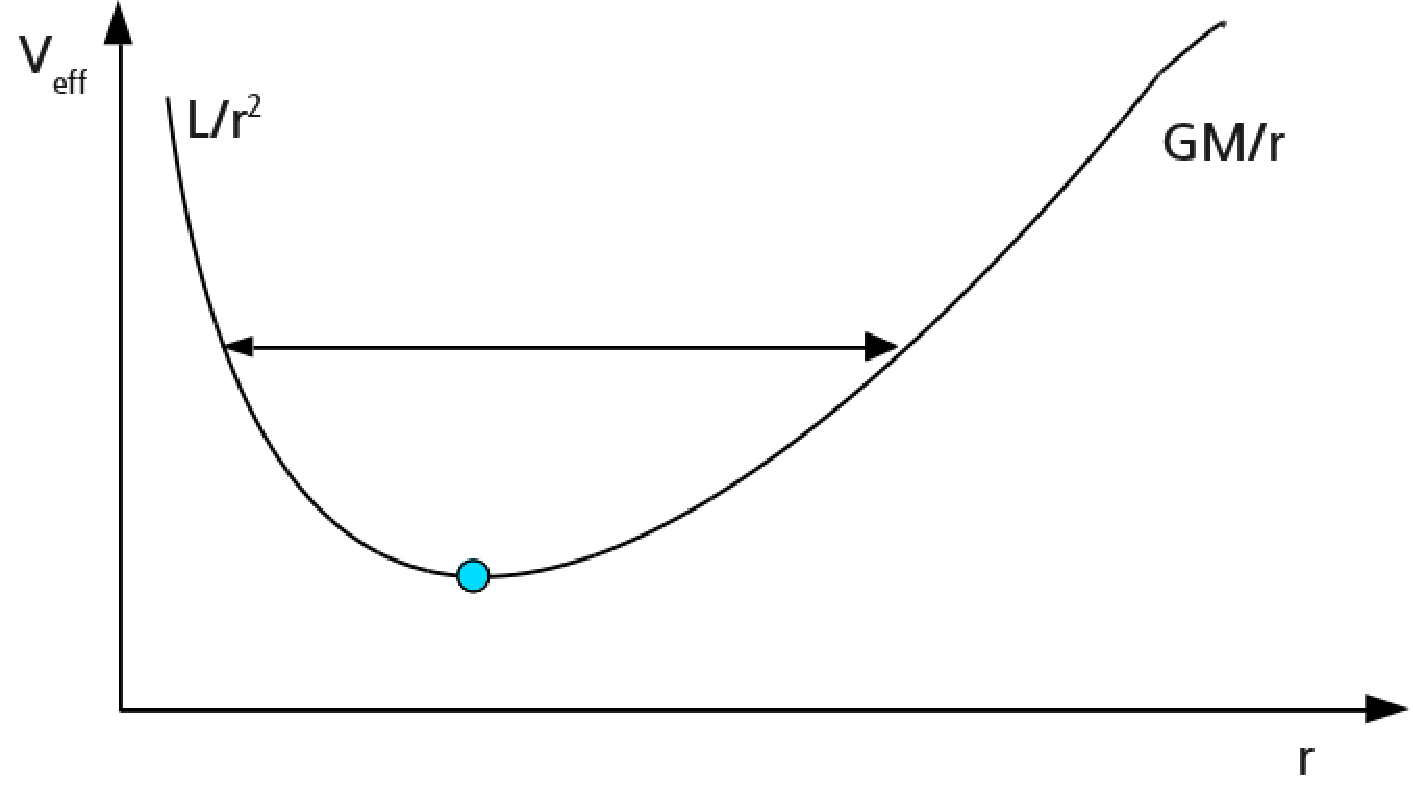
\includegraphics[width=0.7\textwidth]{HighEnergy/angplot}
   \caption{Effective energy with angular momentum, L. Circular orbit will be taken at minimum energy for given L.}
\label{fig:angplot}
\end{figure}

$\Rightarrow$ Crossing eccentric orbits dissipate and circularize.

No centrifugal barrier in vertical direction to counteract z-component of gravity: \textbf{disk formation}
\end{enumerate}

\begin{figure}[!htbp]
   \centering
   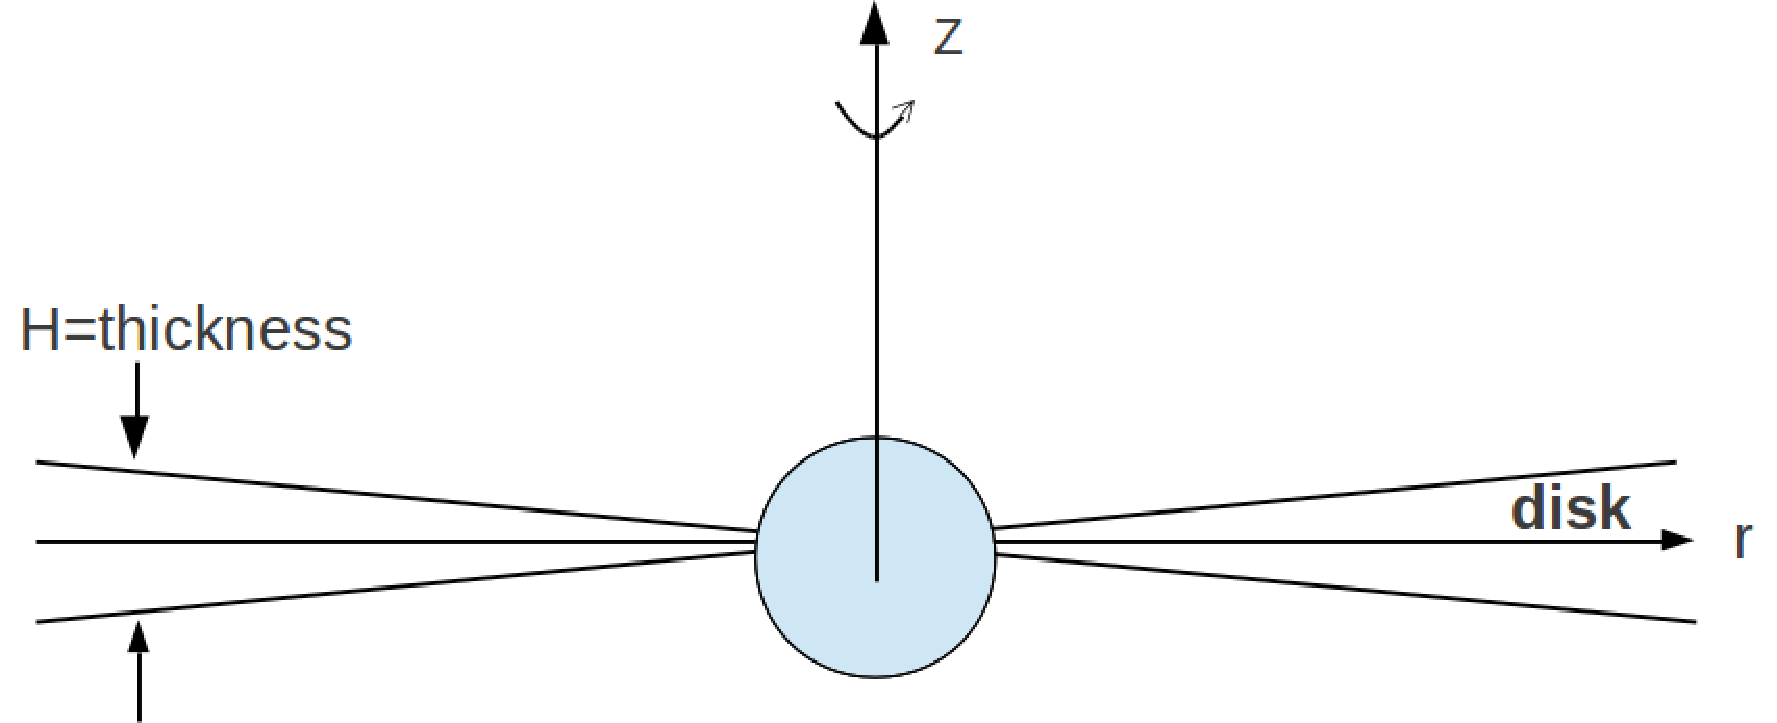
\includegraphics[width=0.7\textwidth]{HighEnergy/disk}
   \caption{Sketch of accretion disk. Centered object will be black hole or neutron star, \ldots. $F_{z}\cong \frac{GM}{r^{2}} \frac{z}{r}$}
\label{fig:disk}
\end{figure}

\textbf{Vertical hydrostatic balance:}

$\Rightarrow$ Only pressure gradient balances vertical gravity.

\begin{figure}[!htbp]
   \centering
   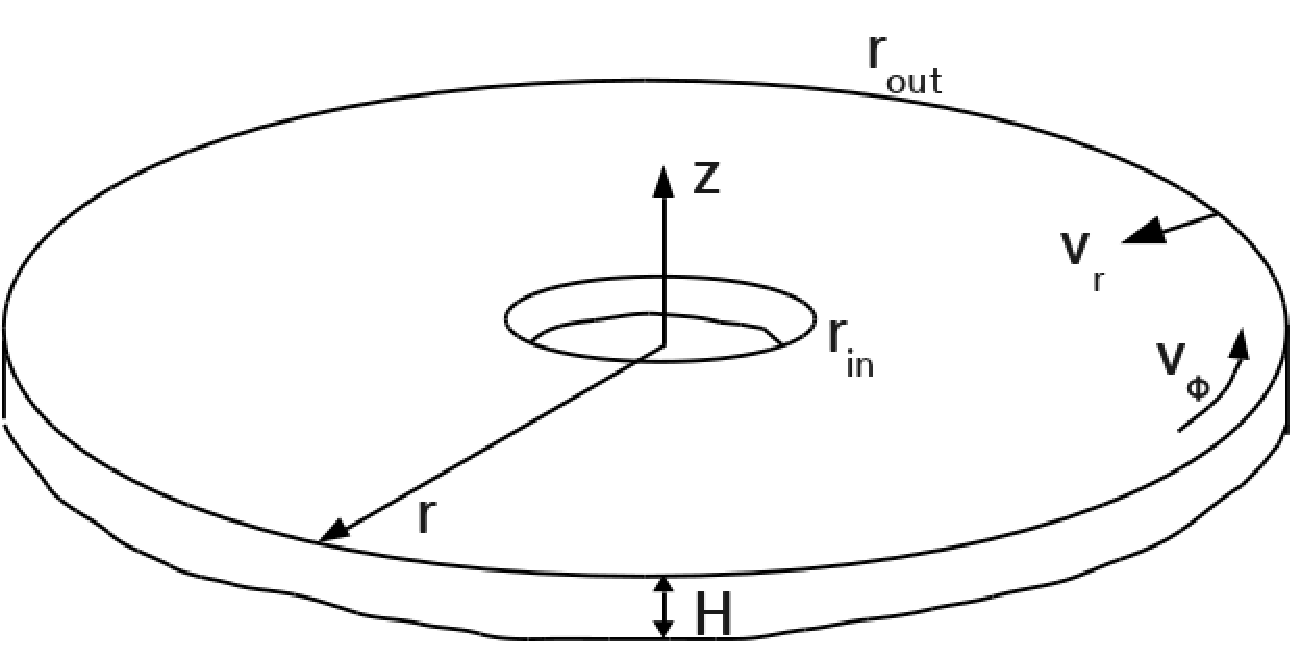
\includegraphics[width=0.7\textwidth]{HighEnergy/accretion}
   \caption{Hydrostatic balance in accretion disk.}
\label{fig:accretion}
\end{figure}

\begin{eqnarray}
   r \Omega &=& v_{\phi} \\
   r \Omega^{2} &=& \frac{GM}{r^{2}}
\end{eqnarray}

\textcolor{red}{
\begin{equation}
   (\text{cf. }L=r^{2}\Omega = r^{2} \sqrt{\frac{GM}{r^{3}}} \propto r^{1/2} ~~\text{for keplerian disk})
\end{equation}
}

The pressure gradient in vertical direction will be balanced by the gravity via
\begin{equation}
   \nabla_{z}P = \frac{\partial}{\partial z}P = \rho g_{z} = -\frac{GM\rho}{r^{2}} \frac{z}{r} = -\rho \Omega^{2}z
\end{equation}

Ansatz: $H \ll r$ and $v_{r} \ll v_{\phi}$.

\begin{equation}
   \Rightarrow ~ \frac{\partial P}{\partial z} \approx -\frac{P}{H} = - \rho \Omega^{2} z \approx -\rho \Omega^{2} H
\end{equation}

\begin{equation}\label{eq:vhse}
   \Leftrightarrow ~ \frac{P}{\rho} \approx \Omega^{2} H^{2} = R^{2} \Omega^{2} \left( \frac{H^{2}}{R^{2}} \right)
   = v_{\phi}^2 \left( \frac{H}{R} \right)^2
\end{equation}
\begin{empheq}[innerbox=\fbox,
left=\Leftrightarrow]{align}
\left( \frac{c_{s}^2}{v_{\phi}^2} \right) \approx \left( \frac{H}{R} \right)^2
\end{empheq}
\begin{equation}
  \Rightarrow ~   v_{\phi} \gg c_{s}  ~\Leftrightarrow~ r \gg H
\end{equation}

Note that assumption of this model is 1) steady state ($\partial / \partial t = 0$), 2) $r \gg H$,and 3) $v_{\phi} \gg v_{r}$.

$\therefore$ Thin accretion disks ($H \ll r$) must be cold ($c_{s} \ll v_{\phi}$).

Also note that a virialized flow would have $c_{s} \approx v_{\phi}$.

\textbf{Order of Magnitude Scaling:}

\begin{enumerate}[a)]
   \item Mass conservation:

   From continuity equation (eq.(\ref{eq:continuity1})), mass transfer rate can be roughly estimated as

\begin{equation}
   \dot{M} = -2\pi R\,H \rho\,v_{R} \equiv -2 \pi R\, \Sigma\, v_{R},
\end{equation}
where $\Sigma$ is surface density. The factor 2 in the equation can be derived by second term in eq.(\ref{eq:continuity1}).
\begin{empheq}[innerbox=\fbox,
left=\Rightarrow]{align}
 \dot{M} \propto R\,\Sigma\,v_{R}
\end{empheq}

   \item Vertical hydrostatic balance:

From the relation ship in eq.(\ref{eq:vhse}),

\begin{equation}
 \Rightarrow ~ \frac{P}{\rho} \sim c_{s}^{2} \propto \Omega^{2} H^{2} \propto v_{\phi}^{2} \left( \frac{H}{R} \right)^2
\end{equation}
\begin{empheq}[innerbox=\fbox,
left=\Rightarrow]{align}
 T \propto \Omega^{2} H^{2}
\end{empheq}
where T is gas pressure dominated temperature in the accretion disk.

   \item Angular momentum conservation:

Advection will be produced by torque
\begin{equation}
  \dot{M} R^{2} \Omega \approx \underbrace{2\pi R\,H}\cdot\underbrace{R}\cdot\underbrace{\rho \nu \frac{\partial \Omega}{\partial R}\,R}
\end{equation}
where LHS is given by derivation of angular momentum, $\partial L / \partial t =\partial
(M\,R^{2}\Omega )/ \partial t$, and in RHS, first term is surface area and second term is lever arm and 
third term is viscous stress. The angular momentum will be transported to outward by viscosity.
\begin{empheq}[innerbox=\fbox,
left=\therefore ~]{align}
 \dot{M} \propto \Sigma\,\nu
\end{empheq}

\item Energy conservation:

Sources = Sinks  ~  ($Q^{+} = Q^{-}$)

Here sources can be gravity and the sinks can be radiation, advection(neglect for now).
\begin{eqnarray}
  Q^{+} &\sim& \frac{d\,E_{pot}}{dt\,dR}dR ~\sim \frac{GM\dot{M}}{R^{2}}dR \\
  Q^{-} &\sim& 2\pi R\,dR \cdot F \sim 2\pi R\,dR \cdot \sigma T_{eff}^{4}
\end{eqnarray}
Under the cool disk assumption, the flux will be dominant for blackbody radiation due to high opacity.
\begin{equation}
   \Rightarrow  ~ T_{eff}^{4} \propto \frac{GM\dot{M}}{R^{3}} \propto \Omega^{2}\dot{M} \propto M\dot{M}R^{-3}
\end{equation}
Interested in $T_{\rm central}$: Optically thick radiation
\begin{figure}[!htbp]
   \centering
   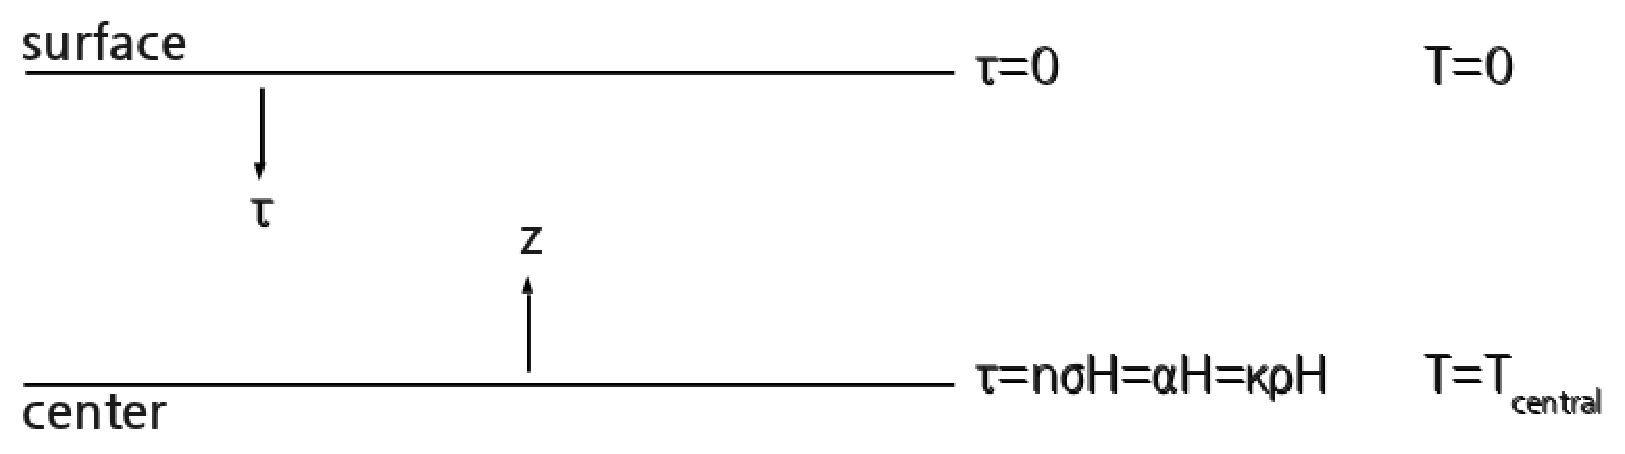
\includegraphics[width=0.7\textwidth]{HighEnergy/thickrad}
   \caption{Sketch of optical depth through disk}
\end{figure}
Radiation escapes from $\tau \le 1$
\begin{equation}
\Rightarrow ~ T_{\rm eff}^{4} \approx T_{\tau=1}^{4} \approx \frac{dT^{4}}{d\tau}\tau_{=1}
\approx \frac{4 T_{central}^4}{\tau_{central}} \approx \frac{4 T_{c}^4}{\kappa \rho H}
\end{equation}
\begin{empheq}[innerbox=\fbox,
left=\therefore ~]{align}
 \frac{T_{c}^4}{\kappa \rho H} \propto \Omega^{2} \dot{M}
\end{empheq}
Note that $\rho H = \Sigma$, so $T_{c}^{4} \propto \kappa \Sigma \Omega^{2} \dot{M}$.

And we will use Kramer's opacity, which is blackbody-weighted absorption.
\begin{empheq}[innerbox=\fbox]{align}
 \kappa_{kr} \propto \rho T^{-7/2} \propto \frac{\Sigma}{H}T^{-7/2}
\end{empheq}

   \item Viscosity: $\nu$ 
\begin{itemize}
   \item Describe microscopic transport of momentum
   \item Characterized by typical transport velocity $\tilde{v}$ and typical random step size $\lambda$:
\begin{equation}
   \nu \approx \lambda \tilde{v}
\end{equation}
   \item Molecular viscosity (kinetic theory):
\begin{equation}
   \nu \approx \lambda_{mfp} c_{s}
\end{equation}
where $\lambda_{mfp}$ is characteristic length of mean free path.

For astrophysical systems of size $l$, often $\lambda_{mfp} \ll l$
\begin{equation}
  \Rightarrow \textrm{Re} \equiv \frac{\textrm{inertial~transport}}{\textrm{viscous~transport}} = \frac{l\,v}{\lambda_{mfp} \cs} \gg 1
\end{equation}
where Re is the Reynolds number.

$\Rightarrow$~~ \textbf{Turbulence !!!!!}

\begin{figure}[!htbp]
   \centering
   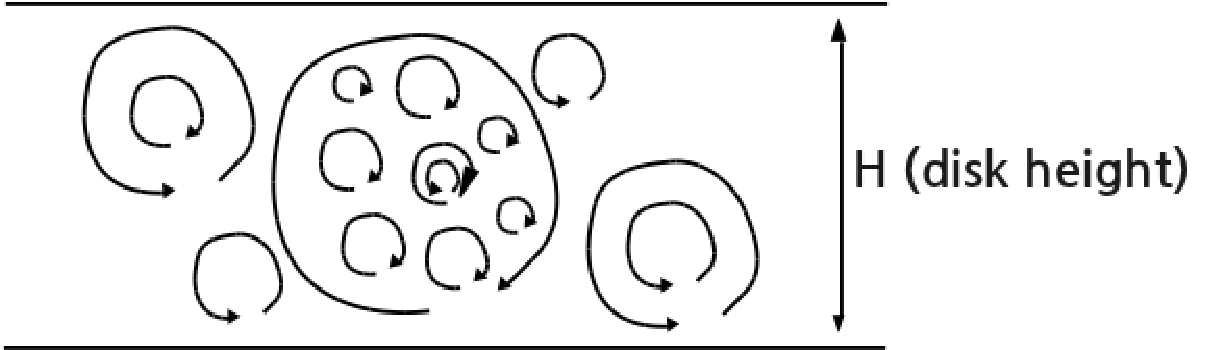
\includegraphics[width=0.7\textwidth]{HighEnergy/eddie}
   \caption{Eddies in the accretion disk. Characteristic length scale is maximum eddie size ($l \approx \rm H$).}
\end{figure}

  \item Characteristic speed: sound speed, $\tilde{v} \approx c_{s}$.
\begin{empheq}[innerbox=\fbox,
left=\therefore ~]{align}
    \nu \equiv \alpha c_{s} {\rm H}, ~~~~ \alpha \le 1
\end{empheq}
Which is \textbf{$\alpha$-disk model}.

   \item viscosity continued: \\
         $\alpha$ contains all uncertainties about $\nu$ very likely smaller than unity ($\alpha \le 1$).
         Very convenient, but \ldots
\end{itemize}
\end{enumerate}

\textbf{Putting it all together:}
\[ \left. 
\begin{array}{ll}
  (1)~~ \dot{M} \sim R \Sigma v_{R} & \rm (mass~ conservation) \\
  (2)~~ H \sim T^{1/2}\Omega^{-1} & \rm (vertical~ structure) \\
  (3)~~ \nu \sim \alpha T^{1/2} H & \rm (\alpha-viscosity) \\
  (4)~~ \dot{M} \sim \Sigma \nu \sim \Sigma \alpha T^{1/2} H & \rm (angular~ momentum) \\
  (5)~~ \frac{T^{4}}{\kappa \Sigma} \sim \dot{M} \Omega^{2} & \rm (energy~ equation) \\
  (6)~~ \kappa \sim \Sigma\,T^{-7/2}H^{-1} & \rm (Kramer's~ opacity)
\end{array} \right. \]

\textbf{Solutions:}

\begin{empheq}[innerbox=\fbox]{align}
 \boldsymbol  T \sim \dot{M}^{3/10} \alpha^{-1/5} M^{1/4} R^{-3/4} \\
 \boldsymbol \Sigma \sim \dot{M}^{7/10} \alpha^{-4/5} M^{1/4} R^{-3/4} \\
 \boldsymbol v_{R} \sim \dot{M}^{3/10} \alpha^{4/5} M^{-1/4} R^{-1/4} 
\end{empheq}
where in the steps, we have used $\Omega \sim  M^{1/2} R^{-3/2}$.

\textbf{Conclusions:}

\begin{enumerate}[1)]
   \item $\alpha$ enters T only marginally.
   \item $v_{R} \sim R^{-1/4}$ but $c_{s} \sim R^{-3/8}$ \\
         $\Rightarrow ~~ \frac{v_{R}}{c_{s}} \equiv M \sim R^{1/8}$ \\
         $\Rightarrow ~~$ less and less supersonic at smaller radius
   \item $v_{R} \sim \alpha^{4/5}$ \\
         $\Rightarrow ~~$ advection becomes more important for large $\alpha$.
\end{enumerate}

\textbf{A complete algebraic solution gives:}

\begin{empheq}[innerbox=\fbox]{align}
  T_{c} &= 1.4\times 10^{4}\,K ~ \alpha^{-1/5} \dot{M}_{16}^{3/10} M^{1/4} R_{10}^{-3/4} f^{6/5}  \\
  v_{R} &= 2.7\times 10^{4}\,cm\,s^{-1} ~ \alpha^{4/5} \dot{M}_{16}^{3/10} M^{-1/4} R_{10}^{-1/4} f^{-14/5} \\
  \tau  &= 33 ~ \alpha^{-4/5} \dot{M}_{16}^{1/5} f^{4/5} \\
  H     &= 1.7\times 10^{8}\,cm ~ \alpha^{-1/10} \dot{M}_{16}^{3/20} M^{-3/8} R_{10}^{9/8} f^{3/5} \\
 \Sigma &=5.2\,g\,cm^{-2} ~ \alpha^{-4/5} \dot{M}_{16}^{7/10} M^{1/4} R_{10}^{-3/4} f^{14/5} 
\end{empheq}
with $\dot{M}_{16} = \dot{M} / 10^{16} \,g\,s^{-1},~M=M_{BH}/M_{\odot},~R_{10}=R/10^{10}\,cm$, \\
and $f=\left[ 1 - \beta \left( R_{i}/R \right)^{1/2} \right]^{1/4}$ where $\beta$ is a viscous coupling constant.\\
Note that $T_{\rm eff}^{4} \sim \Omega^{2} \dot{M} \sim M\dot{M}R^{-3}$, that is independent of $\alpha$!!

\textbf{Spectrum:}
\begin{figure}[!htbp]
   \centering
   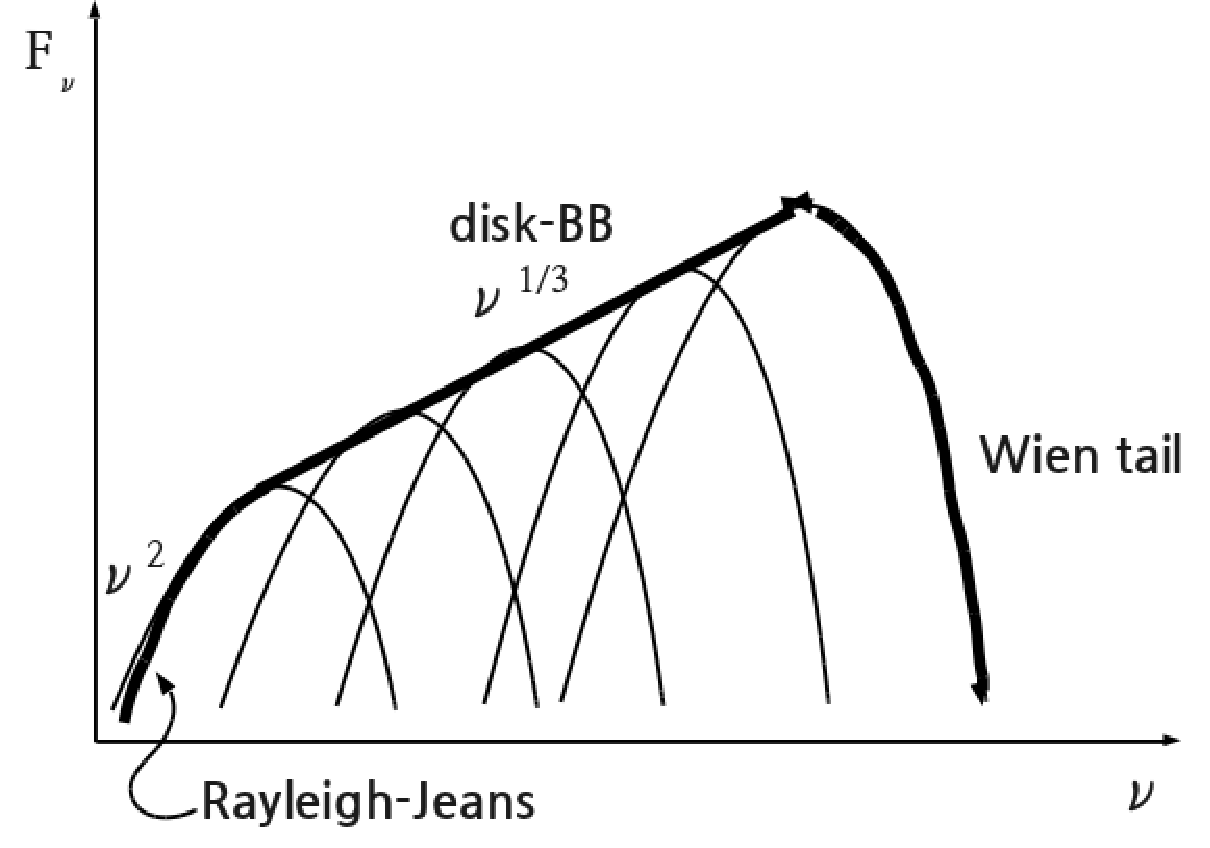
\includegraphics[width=0.65\textwidth]{HighEnergy/bhSpectrum}
   \caption{spectrum from accretion disk}
\end{figure}

The black body spectra from each part of accretion disk are superposed to produce characteristic spectrum.
The higher peak frequency of overlaid spectrum comes from inner disk. 
\[ \left. \begin{array}{ll}
  T_{\rm eff} = 1.3\times 10^{7} \,K ~ \dot{M}_{17}^{1/4} M^{1/4} R_{6}^{-3/4} & \textrm{(neutron star)} \\
  T_{\rm eff} = 1.3\times 10^{5} \,K ~ \dot{M}_{25}^{1/4} M_{8}^{1/4} R_{14}^{-3/4} & (10^{8}\,\unitmsun\,\textrm{black hole)} 
\end{array} \right. \]

\subsubsection{The role of magnetic fields: The magneto-rotational instability}

\begin{enumerate}[a)]
   \item The exact nature of the agent of angular momentum transport was unspecified (hidden in the $\alpha$-parameter)

   $\Rightarrow$~ Magnetic stresses could be responsible:

   A field line anchored into a ring at radius $r$ will co-rotate with this ring. It will try to speed up ring $r_{+}$(outer ring)
   and slow down ring $r_{-}$(inner ring).

   $\Rightarrow$~ angular momentum transport

   From MHD: magnitude of magnetic stress is $\frac{(\vec{B}\cdot\nabla)\vec{B}}{4\pi}$.

   Question: is $\frac{(\vec{B}\cdot\nabla)\vec{B}}{4\pi}$ sufficient, \ie, is B-field large enough?

   Answer: It will be, after a few Keplerian orbits.

   \item \textbf{Magneto-rotational instability (MRI):}

   Consider a vertical field line with a radial perturbation (fig.(\ref{fig:mrivt})).

\begin{figure}[!htbp]
   \centering
   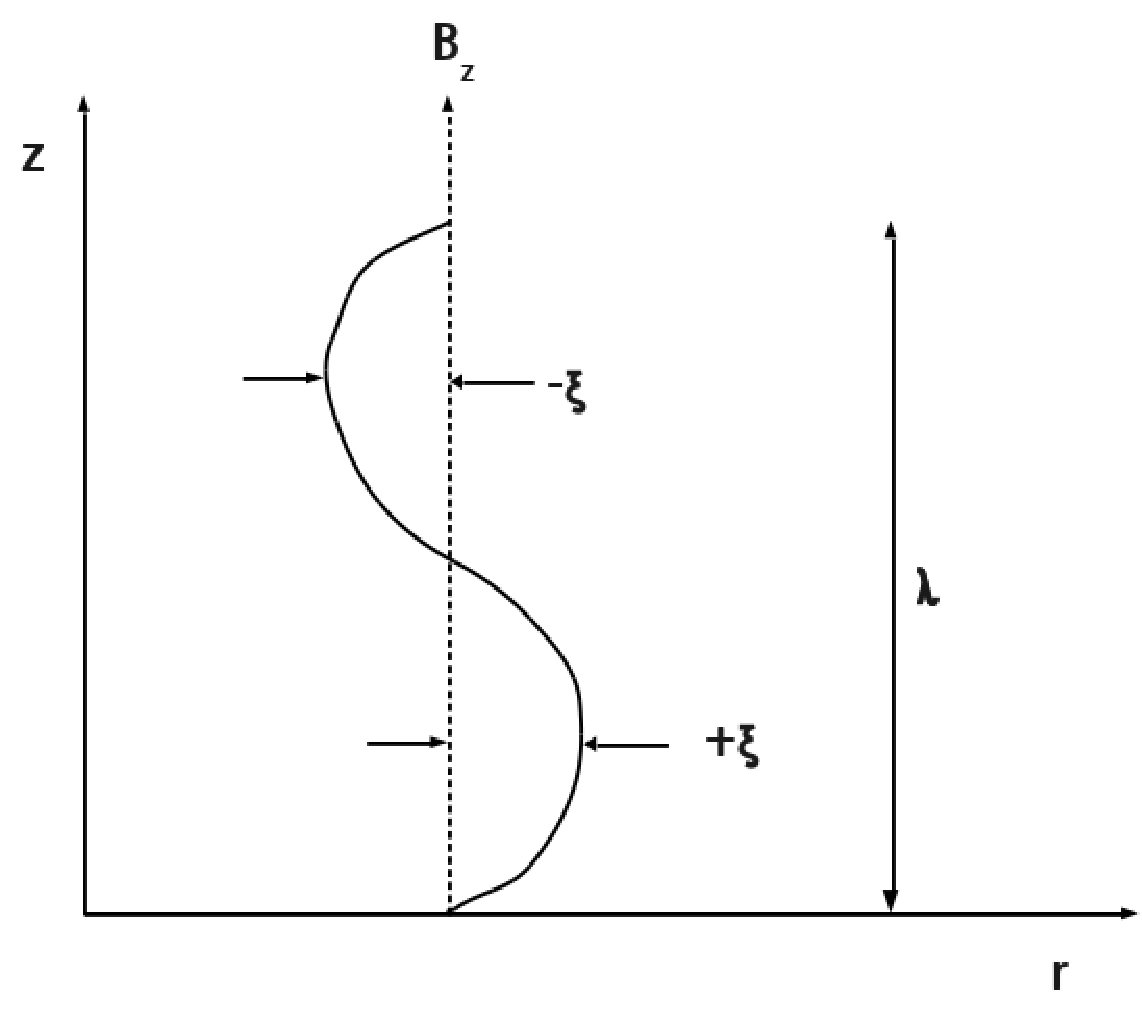
\includegraphics[width=0.7\textwidth]{HighEnergy/mrivt}
   \caption{Vertical magnetic field line}
   \label{fig:mrivt}
\end{figure}

   Here, wavelength $\lambda \le \rm H$ and amplitude(linear regime) $\xi \ll \lambda$.

   Magnetic force density in radial direction is (comment: $B_{r} \sim B_{z} \cdot \frac{\xi}{\lambda}$

\begin{equation}
   f_{B} = \frac{B_{z}}{4\pi}\frac{\partial}{\partial z}B_{r} \sim \frac{B_{z}}{4\pi}\left( - \frac{B_{r}}{\lambda} \right)
        \sim \frac{B_{z}^2}{4\pi}\left( - \frac{\xi}{\lambda^2} \right) \propto - \left( \vec{k}\cdot\vec{v}_{A} \right)^2 \rho\,\xi
\end{equation}
where $v_{A}$ is the \alfven speed, $v_{A}^2 = \frac{B_{z}^2}{4\pi\rho}$.
 
The net centrifugal force resulting from the perturbation is
\begin{equation}
   f_{c} = -\rho R \frac{\partial}{\partial R}(\Omega^{2})\xi = -\rho \frac{d\Omega^{2}}{d\,lnR}\xi
\end{equation}
The centrifugal force excess wins if
\begin{equation}
   f_{c}+f_{B} = -\rho \left( \frac{d \Omega^{2}}{d\,lnR} + \left( \vec{k}\cdot\vec{v}_{A}\right)^2 \right)\xi ~~ (>0\textrm{~for instability})
\end{equation}
which is positive for
\begin{equation}
    \frac{d \Omega^{2}}{d\,lnR} < - \left( \vec{k}\cdot\vec{v}_{A}\right)^2  ~~~ \Rightarrow ~ \textrm{instability}
\end{equation}
So there is a minimum wavelength (maximum $k$) for which the instability grows and we need
\begin{equation}
   \frac{d\Omega^{2}}{dR} < 0 
\end{equation}
with $\frac{B_{z}^{2}}{\lambda_{z}^{2}\rho} \le \Omega^{2}$ or $\lambda_{z}^2 \ge \frac{B_{z}^{2}}{\Omega^{2}\rho}$.
So unstable as long as ${\rm H} \ge \lambda_{\rm min}$ or ${\rm B} \le \textrm{equipartition}$.
(because $B^{2} \le {\rm H}^{2} \Omega^{2}\rho \le P$, where ${\rm H}^{2}\Omega^{2}=c_{s}^2$ in equipartition).

\end{enumerate}

\subsubsection{Other accretion regimes}

\noi We have neglected (among other things):

\begin{itemize}
   \item the inner boundary
   \item radiation pressure
   \item advection of energy
   \item time dependence
   \item non-local dissipation (B-fields), \ie, magnetic reconnection
\end{itemize}

\begin{enumerate}[a)]
   \item Radiation pressure:
   
\begin{equation}
   P_{\rm thermal} \propto T ~~~ vs. ~~~ P_{rad} \propto T^{4}
\end{equation}
   
Since, for the standard thin disk $T \sim \dot{M}^{3/10} \alpha^{-1/5} M^{1/4} R^{-3/4}$, the radiation 
pressure must dominate at large $\dot{M}$, small R.

It is straight forward to re-do the analysis by replacing the pressure term $\frac{a T^{4}}{3}$, but 
hardly worth is:

\textit{Radiation pressure supported disks are thermally and viscously unstable.}

$\Rightarrow$ equilibrium solution is never established.

Note: an accretion disk is anisotropic, so in principle, it can exceed the Eddington limit by a factor of a few.

   \item \textbf{Advection Dominated Accretion Flows (ADAFs)}

We have neglected energy advection $Q_{Adv}^{-}$ in the energy balance. The advective term becomes important
in (a) high $\dot{M}$ cases, where it can alleviate the Eddington limit and (b) low $\dot{M}$, high $\alpha$ cases.

Advection always decreases the radiative efficiency of the flow.

Advection dominated solution:
\begin{eqnarray}
   Q_{Adv}^{-} &\sim& \Sigma\,T\, 2\pi R v_{R} \sim T \dot{M} \\
   Q_{Adv}^{+} &\sim& \frac{G M \dot{M}}{R}
\end{eqnarray}

Balance:
\begin{equation}
  T \sim \frac{GM}{R}\sim \Omega^2 R^2 \sim T_{virial} ~~~\textrm{(hot)}
\end{equation}
and with vertical hydrostatic balance: $T\sim\Omega^2 H^2$
\begin{equation}
  H \sim T^{1/2} \Omega^{-1} \sim R ~~~ \rm (thick~disk~~ (cf.~ thin~ \leftarrow~ radiative~ dominate))
\end{equation}
so 
\begin{equation}
   v_{R} \sim \frac{\dot{M}}{\Sigma\,R}
\end{equation}
and
\begin{equation}
  \dot{M} \sim \Sigma \nu \sim \Sigma \alpha T^{1/2} H
\end{equation}
\begin{eqnarray}
   \Rightarrow ~~ v_{R} &\sim& \frac{\dot{M}}{\Sigma R} \sim \frac{\Sigma \alpha T^{1/2} H}{\Sigma R} 
                            \sim \alpha T^{1/2}H/R \nonumnext
                        &\sim& \alpha\Omega R \sim \alpha v_{\phi} ~~~~~~~~~~~~~(\textrm{rapid inflow})
\end{eqnarray}
Thus: Advection Dominated Accretion Flows are
\begin{itemize}
   \item hot (roughly at Virial temperature), $T \sim T_{\rm vir}$
   \item thick (not so much disk-like, more spherical), H$\,\sim\,$R
   \item non-Keplerian  (radial velocity comparable to $v_{\phi}$)
   \item require large $\alpha$
\end{itemize}
Note: ADAFs require radiative losses to be inefficient.

In a hot flow, it is possible that ions and electrons are thermally decoupled. If the ions get heated,
they might not transfer their energy to the electrons, who do all the radiating

$\Rightarrow$ ~~ Very hot flow implies strong Compton emission

$\Rightarrow$ ~~ Power-law emission (low-hard state ?)

As of today, it is not clear whether electrons and ions are really that strongly decoupled.

   \item The inner boundary: \\
We have neglected entirely what happens at the inner boundary. Introduces correction
\textcolor{red}{$\vartheta(r_{i}/r)$}\ldots

\begin{enumerate}[i)]
\item Neutron stars; WDs:

   Boundary layer must spin incoming material up or down to co-rotate with NS $\Rightarrow$ dissipation.

   Residual kinetic and thermal energy must be dissipated and radiated (\ie, no true advection).

\item Black holes:

   Usual assumption: zero-torque at marginally stable circular orbit (still introduces correction of order
   $r_{i}/r$ to solution)

   Energy can be advected across horizon.

   $\Rightarrow$ are low luminosity sources advection dominant?

   $\Rightarrow$ are black holes in quiescence dimmer than NS in quiescence because they have an event horizon? 

But note: \textbf{``The absence of evidence is not the evidence of absence.}

In other words, black holes could be dim for other reasons, their dimness is no proof for the
existence of event horizons (sadly, some might say) \end{enumerate}


\begin{figure}[!htbp]
   \centering
   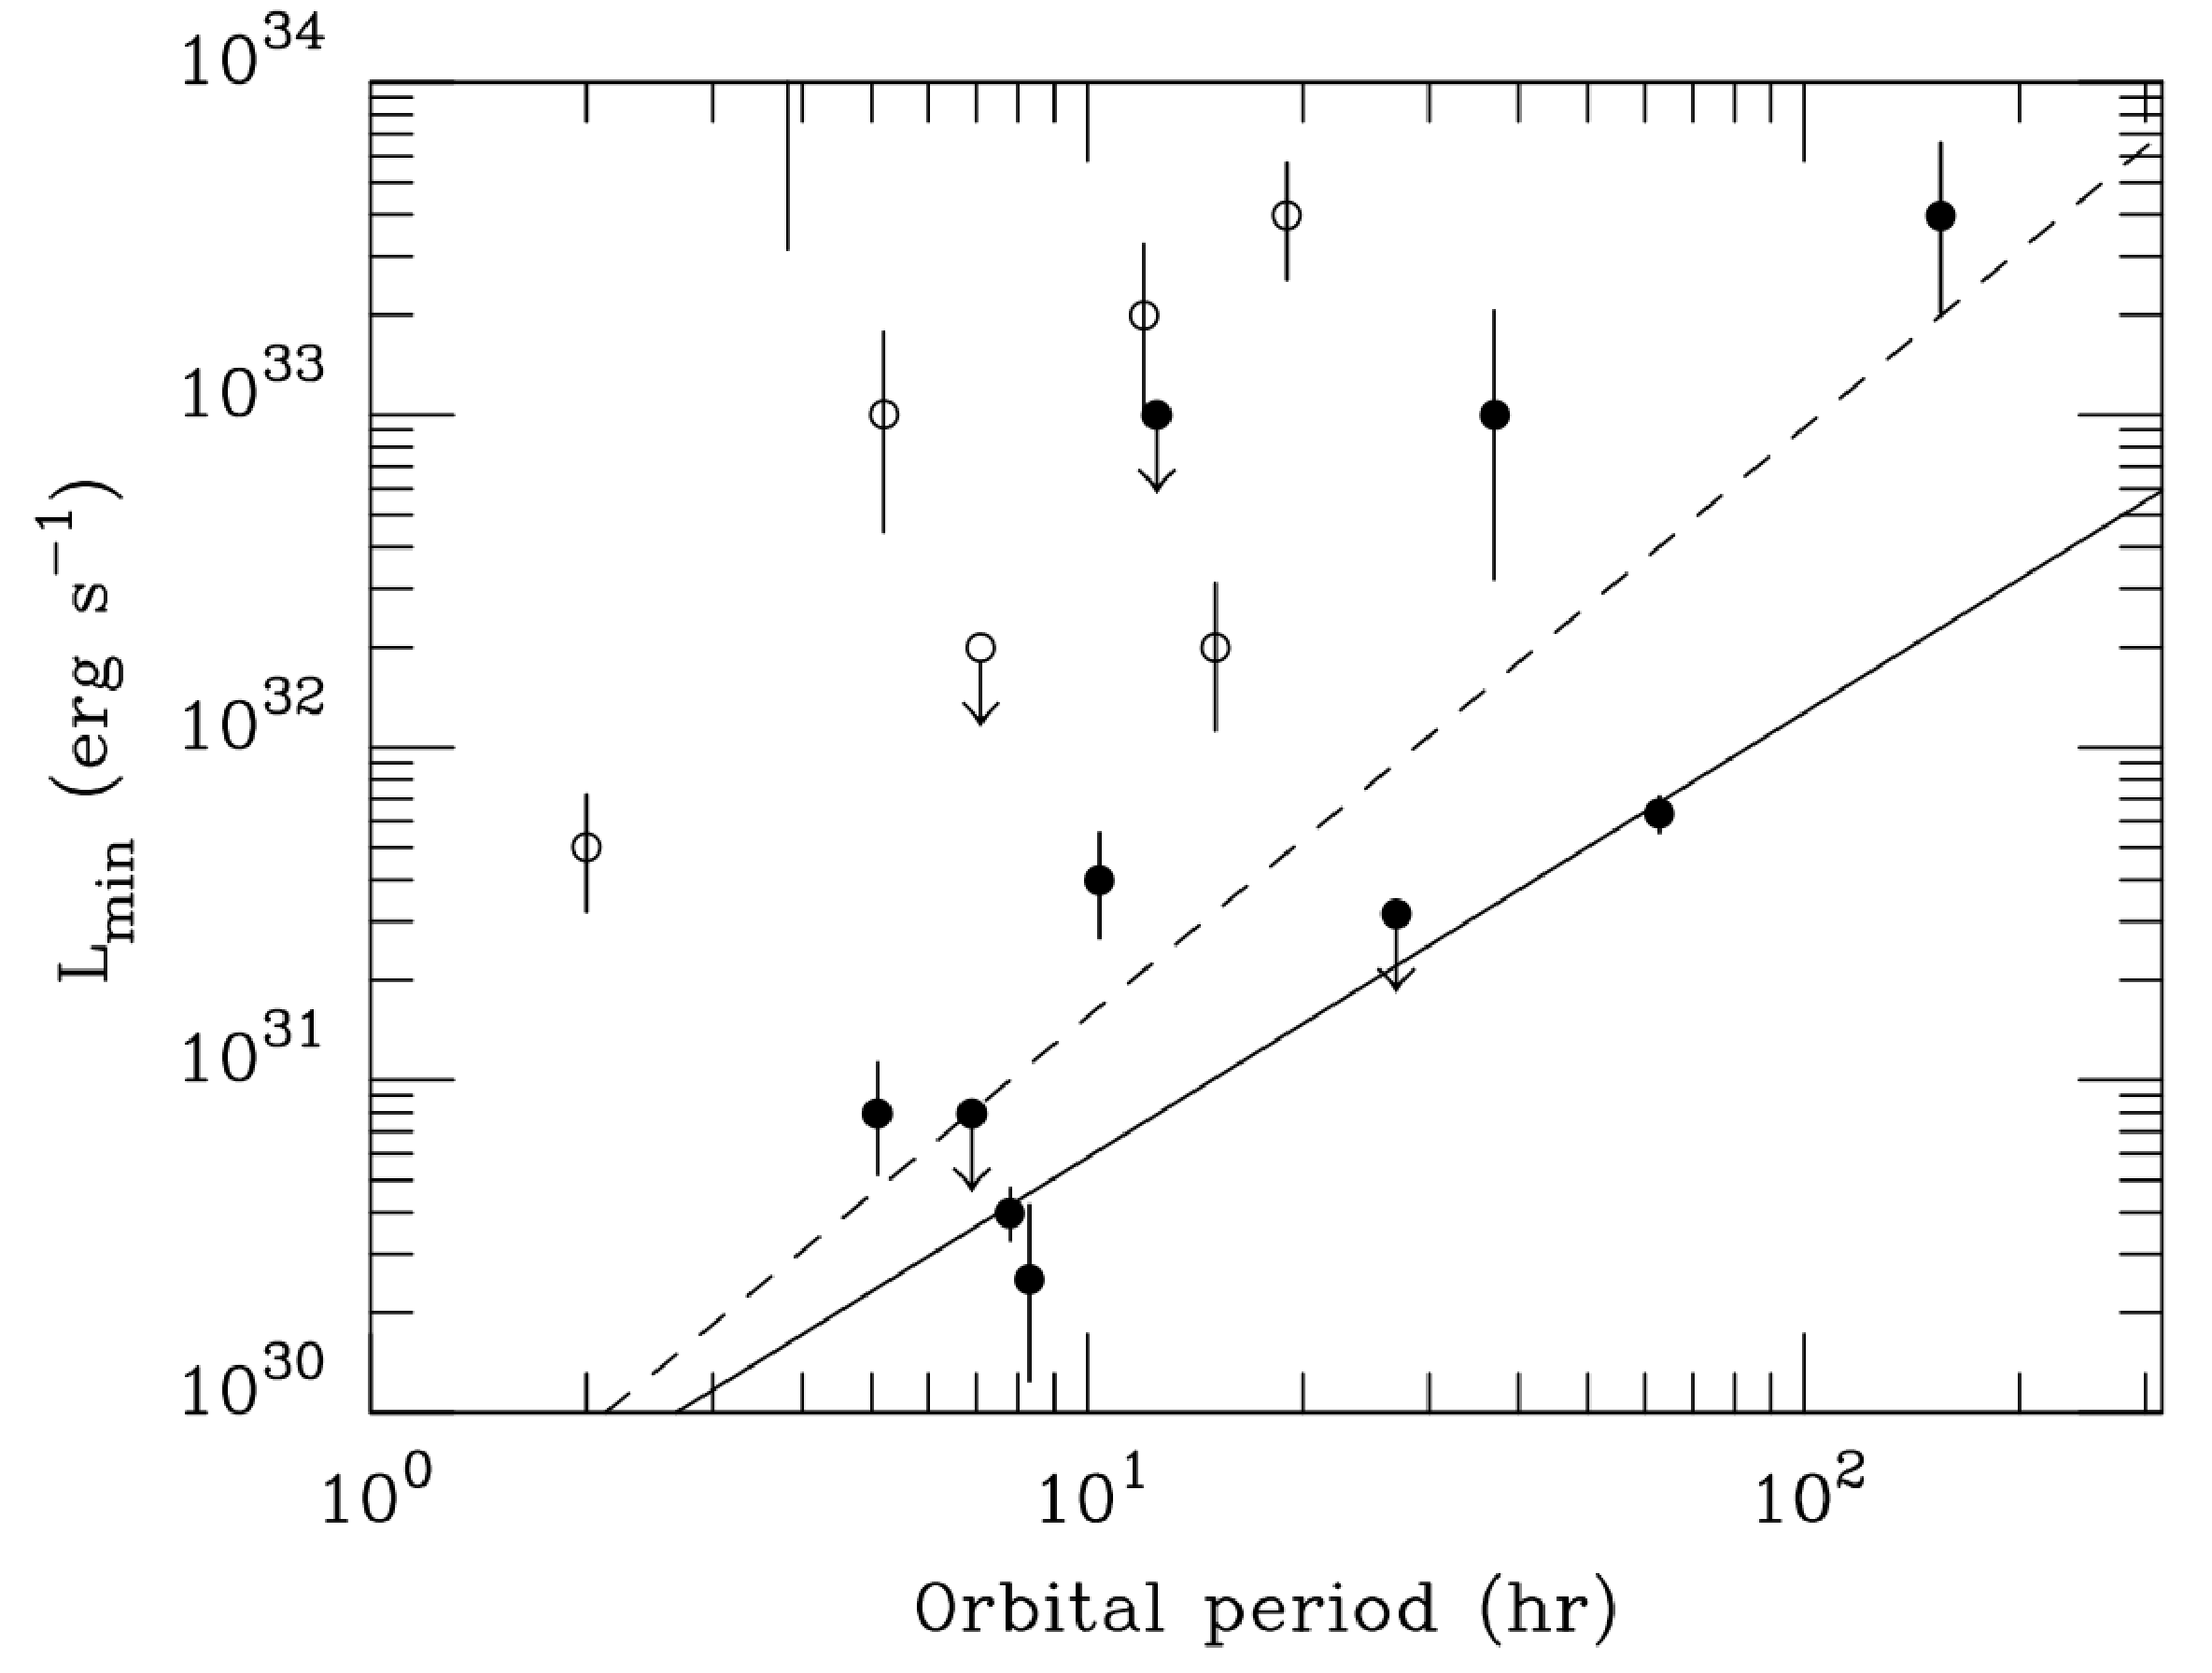
\includegraphics[width=0.7\textwidth]{HighEnergy/Hameury_03}
   \caption{XRBs in quiescence (Hameury et al. 2003). Open circles represent neutron stars and filled circles represent black holes. }
\label{fig:NsBh}
\end{figure}

   \item Typical time scales

\begin{enumerate}[1)]
   \item Signal propagation:
   
\begin{eqnarray}
   \tau_{visc} &\sim& \frac{M}{\dot{M}} \sim \rho \frac{R^{2}H}{\Sigma \nu} \sim \frac{\Sigma R^{2}}{\Sigma \nu} \nonumnext
               &\sim& \frac{R^{2}}{\nu} \approx 5\times 10^5 ~ R_{10}^{10/8} M^{2/8}\, \dot{M}_{16}^{-3/10} \alpha^{-4/5}
\end{eqnarray}
Recall: $\nu$ has units length$^2$/time.

$\tau_{visc}$ is the time it takes for the disk to be drained completely if the accretion source turns off
(\eg, mass transfer from companion star)

   \item Thermal (Kelvin-Helmholtz) time:

\begin{eqnarray}
   \tau_{th} &\sim& \frac{E_{th}}{\dot{E}} \sim \frac{\rho c_{s}^{2} R^{2} H}{GM\dot{M}/R} \sim \frac{\Sigma c_{s}^{2}R^{3}}{CM\Sigma \nu} \nonumnext
             &\sim& \frac{\Sigma c_{s}^{2}}{\Sigma \nu \Omega^{2}} \sim \frac{c_{s}^{2}R^{2}}{\nu R^{2}\Omega^{2}} \sim \frac{c_{s}^{2} R^{2}}{\nu v_{\phi}^2}
\end{eqnarray}
\begin{equation}
   \therefore \tau_{th} \sim \tau_{visc} \left( \frac{c_{s}^{2}}{v_{\phi}^{2}} \right) \ll \tau_{visc}
\end{equation}

$\Rightarrow$ Thermal evolution much more rapid than viscous for thin disks.
\end{enumerate}

   \item Non-local dissipation - corona

\begin{figure}[!htbp]
   \centering
   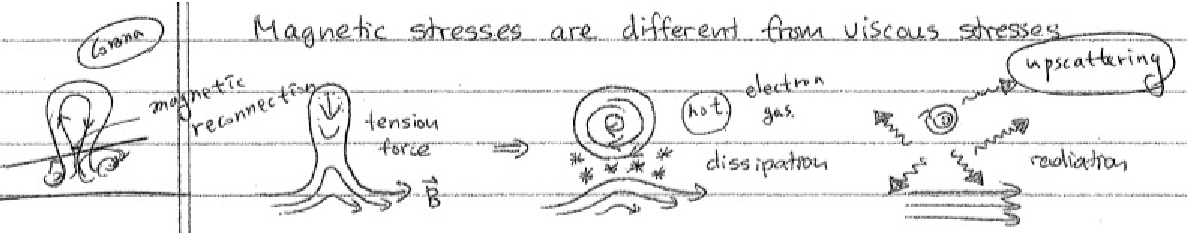
\includegraphics[width=\textwidth]{HighEnergy/note01}
   \caption{Magnetic stresses are different from viscous stresses}
\end{figure}

If viscosity is magnetic, dissipation will be dominated by reconnection.

$\Rightarrow$ Dissipation independent of $\rho$, field lines can rise out of disk and dissipate.

$\Rightarrow$ A layer of hot, low density gas will form above the disk - a ``coronae'' (See the Sun)

Emission: Soft photons from disk are Compton-upscattered (See fig.(\ref{fig:coronae}))
\begin{figure}[!htbp]
   \centering
   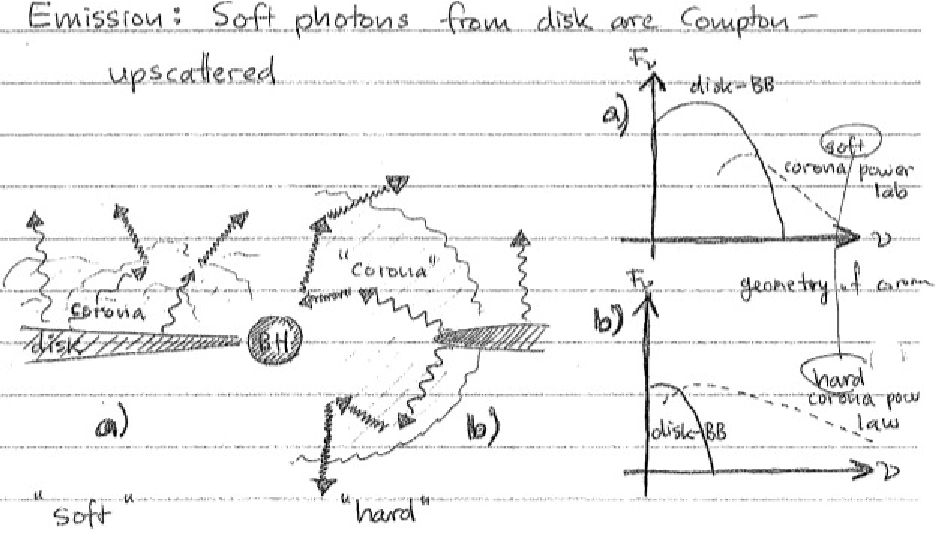
\includegraphics[width=\textwidth]{HighEnergy/note02}
   \caption{Emission: Soft photons from disk are Compton-upscattered}
   \label{fig:coronae}
\end{figure}

\end{enumerate}

\subsubsection{Viscosity Shear Stress: Spherical Coordinate}

The tensors are working on both the momentum equation for angular momentum transport and 
the energy equation for viscous heating \cite{Stone:99}:

\begin{equation}\label{eq:mom}
    \rho \frac{d \vec{v}}{d t} = - \nabla P - \rho \nabla \Phi + \nabla \cdot \boldsymbol{T}
\end{equation}
\begin{equation}
    \rho \frac{d(e/\rho)}{dt} = -P \nabla \cdot \vec{v} + \boldsymbol{T}^{2}/\mu
\end{equation}
where $\boldsymbol{T}$ is an anomalous stress tensor, and $\mu = \rho \nu$ is the coefficient of shear viscosity,
and $\nu$ is the kinematic viscosity coefficient:
\begin{equation}
    \nu = \frac{\alpha \, c_{s}^{2}}{\Omega_{\rm k}}
\end{equation}
where $c_{s}$ is the sound speed of the medium, $\alpha$ is a conventional parameter for thin
disk model by \cite{Shakura:73}.  and $\Omega_{\rm k}$ is the keplerian angular velocity,
\begin{equation}
    \Omega_{\rm k} = \left( \frac{1}{r} \frac{\partial \Phi}{\partial r} \right)^{1/2},
\end{equation}

In spherical coordinates, the shear stress elements can be expressed as:
\begin{equation}
    \boldsymbol{T}_{r\theta}=\boldsymbol{T}_{\theta r} = 
         \mu \left\{ r \frac{\partial}{\partial r} \left( \frac{v_{\theta}}{r} \right) + \frac{1}{r} \frac{\partial v_{r}}{\partial \theta}  \right\}
\end{equation}
\begin{equation}
    \boldsymbol{T}_{r\phi}=\boldsymbol{T}_{\phi r} = 
         \mu \left\{ r \frac{\partial}{\partial r} \left( \frac{v_{\phi}}{r} \right) + \frac{1}{r \sin{\theta}} \frac{\partial v_{r}}{\partial \phi}  \right\}
\end{equation}
\begin{equation}
    \boldsymbol{T}_{\theta\phi}=\boldsymbol{T}_{\phi\theta} = 
         \mu \left\{ \frac{\sin{\theta}}{r} \frac{\partial}{\partial \theta} \left( \frac{v_{\phi}}{\sin{\theta}} \right) + \frac{1}{r \sin{\theta}} \frac{\partial v_{\theta}}{\partial \phi}  \right\}
\end{equation}
These derived tensors were confirmed by \cite{Okuda:97} (note that there are some typos in the equations of the paper). 
Since we are considering 2-D simulation ($r,\theta$), $\partial/\partial{\phi}$ term in the equations above can be neglected.

The divergence of a tensor is 
\begin{equation}
    \nabla \cdot \boldsymbol{T} = \frac{\partial T_{ij}}{\partial x_{j}} \, \boldsymbol{e}_{i}.
\end{equation}
Using this tensor calculus, the tensor term in eq.~(\ref{eq:mom}) can be expressed as
\begin{align}\label{eq:fullT}
    \nabla \cdot \boldsymbol{T} =& 
    \left\{ \frac{\partial T_{rr}}{\partial r} + \frac{1}{r}\frac{\partial T_{r\theta}}{\partial \theta} 
    + \frac{1}{r\sin{\theta}}\frac{\partial T_{r\phi}}{\partial \phi} 
    + \frac{2\,T_{rr}+\cot{\theta}\,T_{r\theta}-T_{\theta\theta}-T_{\phi\phi}}{r}  \right\}\,\hat{r} \\ 
   &+ \left\{ \frac{\partial T_{\theta r}}{\partial r} + \frac{1}{r}\frac{\partial T_{\theta\theta}}{\partial \theta} 
    + \frac{1}{r\sin{\theta}}\frac{\partial T_{\theta\phi}}{\partial \phi} 
    + \frac{T_{r\theta}+2T_{\theta r}+\cot{\theta}(T_{\theta\theta}-T_{\phi\phi})}{r}  \right\}\,\hat{\theta}  \nonumnext
   &+ \left\{ \frac{\partial T_{\phi r}}{\partial r} + \frac{1}{r}\frac{\partial T_{\phi\theta}}{\partial \theta} 
    + \frac{1}{r\sin{\theta}}\frac{\partial T_{\phi\phi}}{\partial \phi} 
    + \frac{T_{r\phi}+2T_{\phi r}+\cot{\theta}(T_{\theta\phi}+T_{\phi\theta})}{r}  \right\}\,\hat{\phi}.  \nonumber 
\end{align}
Applying $T_{r\theta}=T_{\theta r}$, $T_{r\phi}=T_{\phi r}$, $T_{\theta\phi}=T_{\phi\theta}$ and
ignoring normal stress terms and $\partial/\partial \phi$ terms, the eq.~(\ref{eq:fullT}) can be rewritten as

\begin{align}\label{eq:partT}
    \nabla \cdot \boldsymbol{T} =& 
    \left\{ \frac{1}{r}\frac{\partial T_{r\theta}}{\partial \theta} 
    + \frac{\cot{\theta}\,T_{r\theta}}{r}  \right\}\,\hat{r} \\ 
   &+ \left\{ \frac{\partial T_{r \theta}}{\partial r} 
    + \frac{3\,T_{r\theta})}{r}  \right\}\,\hat{\theta}  \nonumnext
   &+ \left\{ \frac{\partial T_{r \phi}}{\partial r} + \frac{1}{r}\frac{\partial T_{\theta\phi}}{\partial \theta} 
    + \frac{3\,T_{r\phi}+2\,\cot{\theta}\,T_{\theta\phi}}{r}  \right\}\,\hat{\phi}.  \nonumber 
\end{align}

The angular momentum transport ($\hat{\phi}$) by the stress tensor can be explained by several mechanisms:
magneto-rotational instability, gravitational instability, and asymmetric gravitational torque.
However, the way of momentum loss in other components is not clear. 

\bigskip
\subsection{Jets}

In accretion physics, the motivation was predominantly theoretical in nature. (\ie, we knew
material must fall into the potential wall of the compact object, conserving angular momentum
$\Rightarrow$ accretion), supported by a body of circumstantial evidence (spectra, luminosity,
variability). We know why accretion happens.

In jet physics, the situation is reversed. We know that jets exist primarily from an observational 
point of view (unlike accretion flows, they are resolved), but we don't know why.
\begin{empheq}[innerbox=\fbox,
left=\Rightarrow]{align}
~~\textrm{Phenomenological approach to understanding jets} \nonumber
\end{empheq}

\subsubsection{Phenomenology}

   \begin{enumerate}[a)]
      \item jets in astrophysical systems 
      \begin{itemize}
          \item classic radio loud AGN ($\ge$ 10\%)
          \item X-ray binaries
             \subitem - black holes ~~(essentially all)
             \subitem - neutron stars (Z-sources)
             \subitem - white dwarfs ~(some CVs)
          \item Gamma ray bursts (100\%)
          \item Proto-stars
          \item Pulsars ?
      \end{itemize}
   The ultimate test for the presence of a jet is still the resolved image of an elongated (\ie, collimated)
   structure pointing away from a point source.

\begin{figure}[!htbp]
   \centering
   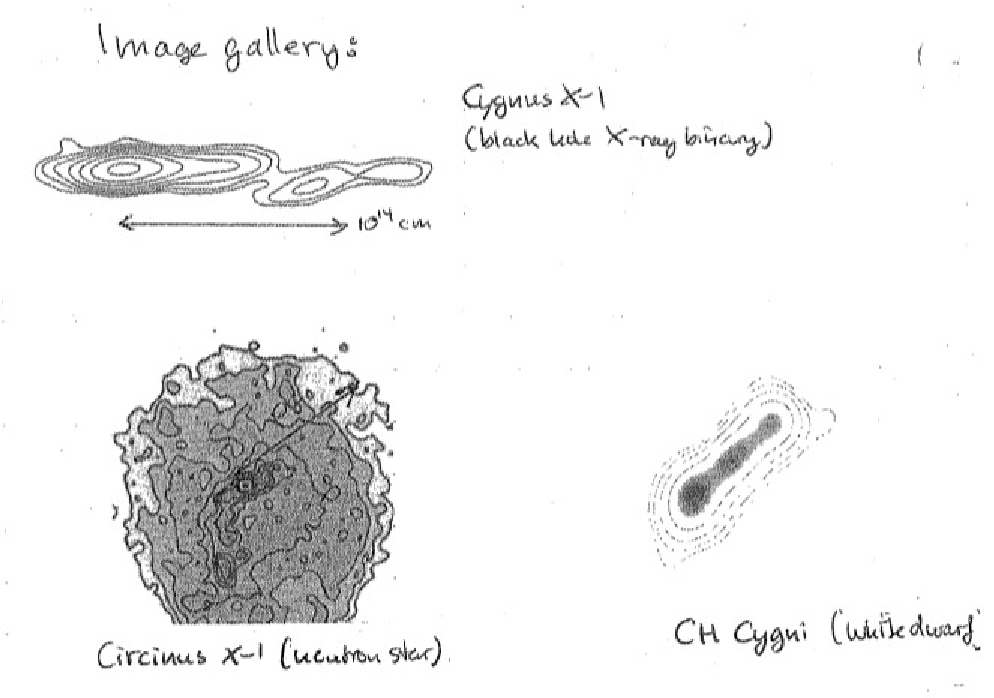
\includegraphics[width=0.7\textwidth]{HighEnergy/note03}
   \caption{Top:Cygnus X-1, bottom-left: Circinus X-1 (neutron star), bottom-right: CH Cygni (White dwarf)}
\end{figure}

\textbf{Morphology (See table (\ref{tab:agn}))}

   \begin{table}[ht]
   \caption{Fanaroff-Riley classification of radio galaxies (See fig.(\ref{fig:FR}))}
   \centering
   \begin{tabular}{cc}
   \hline \hline
   Type I & Type II \\ [0.5ex]
   \hline
   Brighter on smaller scales & Brighter on larger scales \\
   Jet brighter than lobe     & Jet dimmer than lobe      \\ 
   Often two-sided jets       & Most often one-sided jets \\
   Often bent jets            & Straight jets             \\ [1ex]
   \hline
   \end{tabular}
   \label{tab:agn}
   \end{table}

\begin{figure}[!htbp]
   \centering
   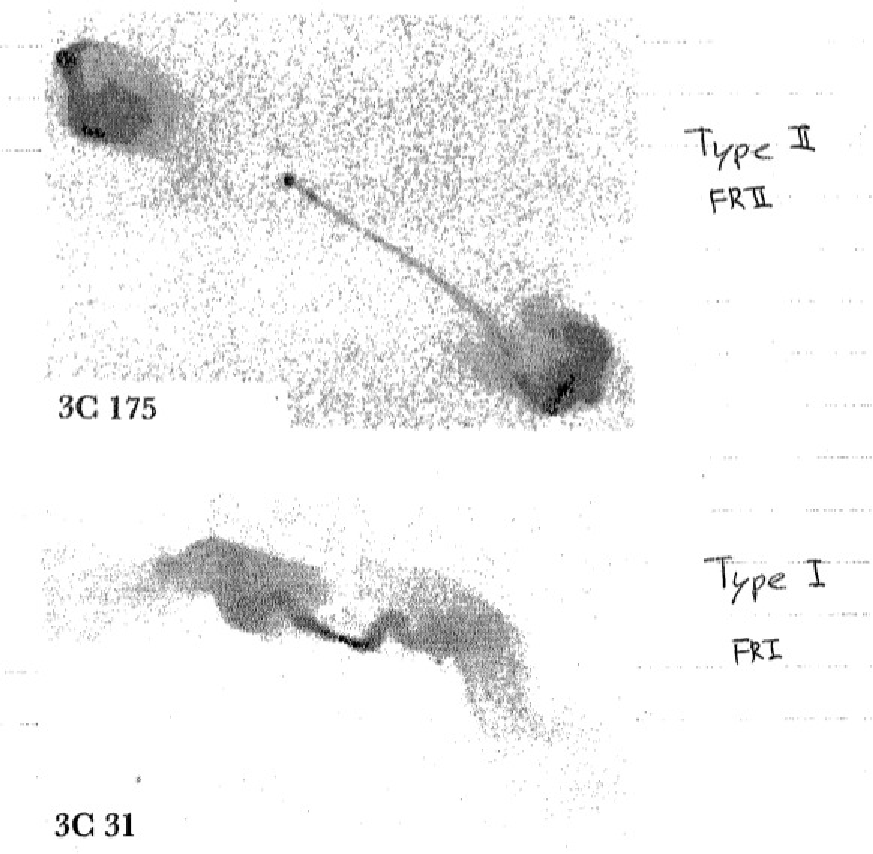
\includegraphics[width=0.7\textwidth]{HighEnergy/note04}
   \caption{Top: FRII galaxy, bottom: FRI galaxy}
\label{fig:FR}
\end{figure}

\begin{figure}[!htbp]
   \centering
   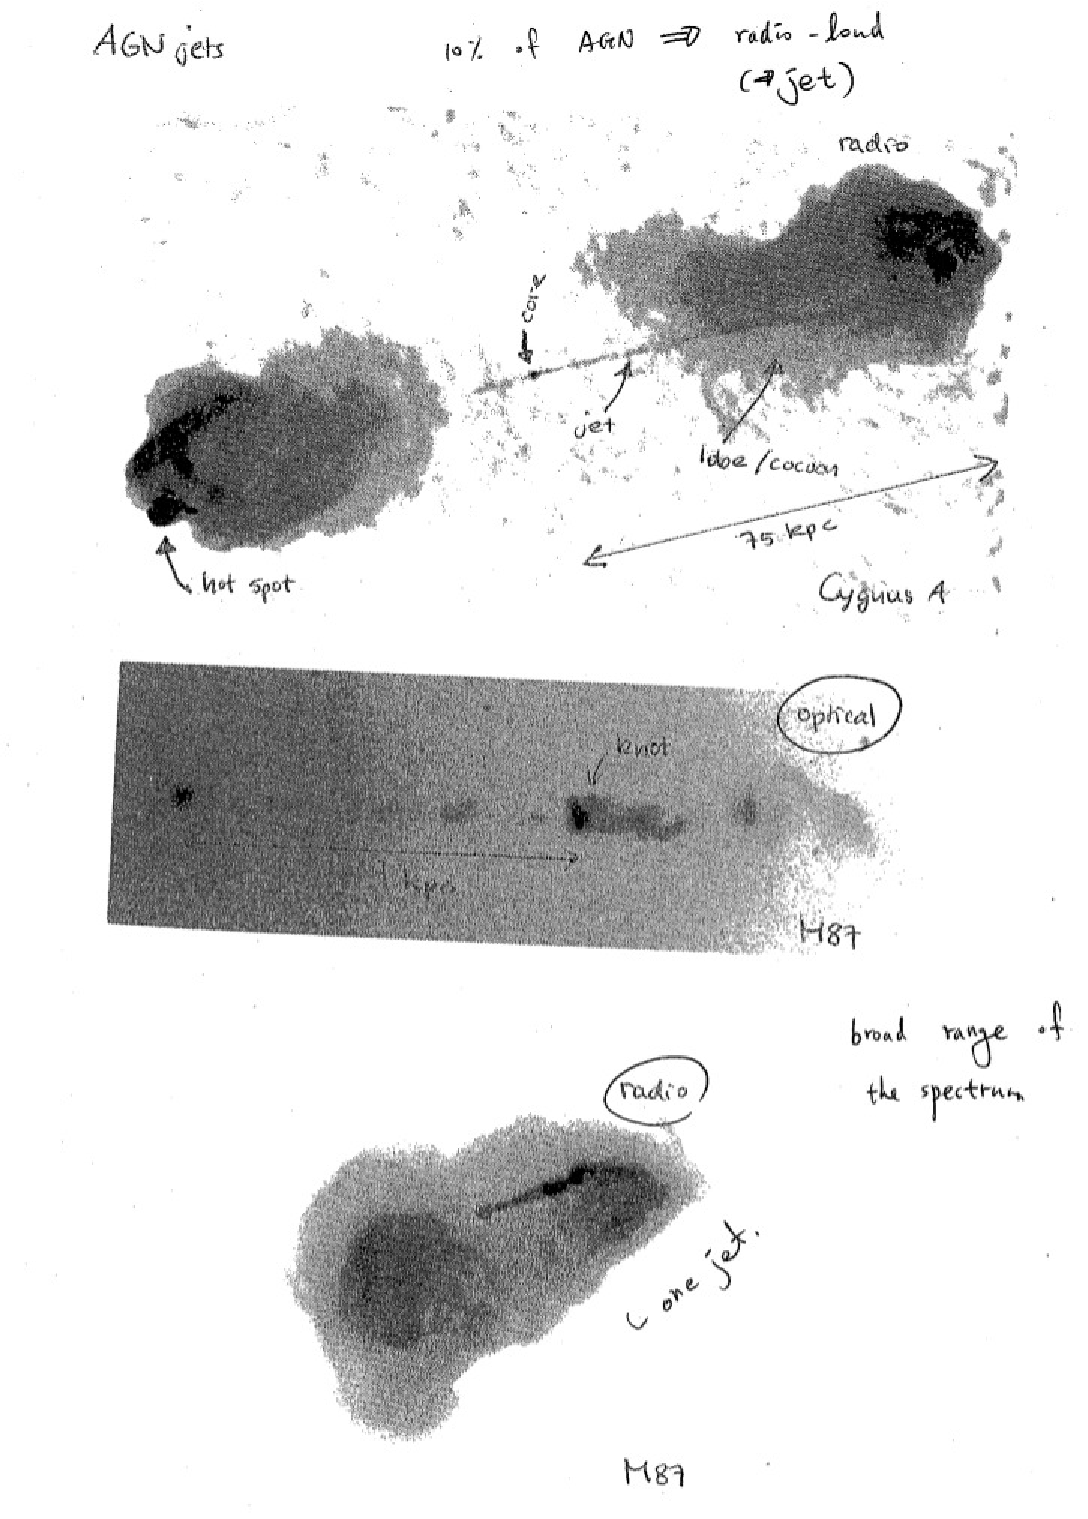
\includegraphics[width=\textwidth]{HighEnergy/note05}
   \caption{AGN jets}
\label{fig:angjets}
\end{figure}

\begin{figure}[!htbp]
   \centering
   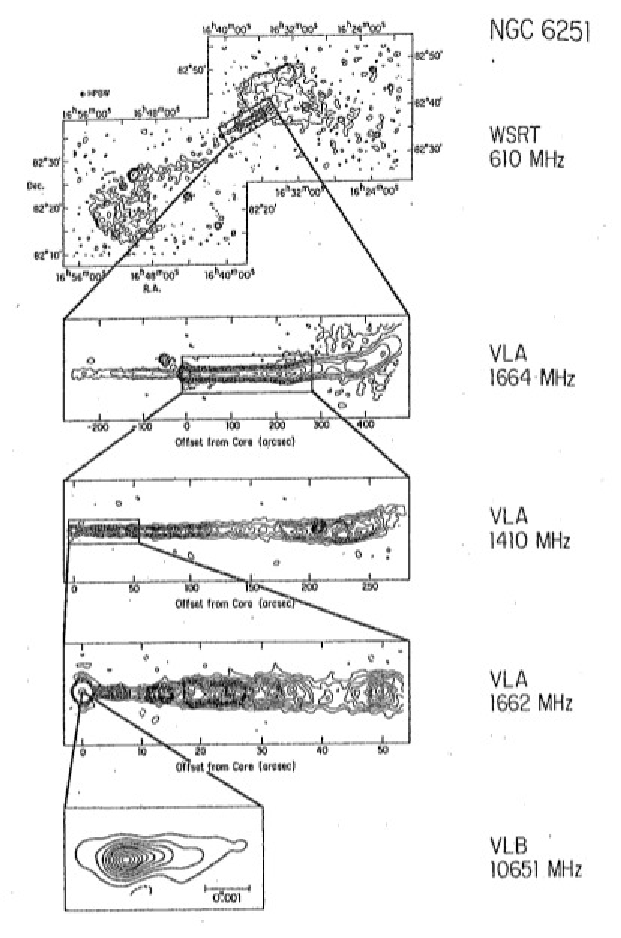
\includegraphics[width=0.9\textwidth]{HighEnergy/note06}
   \caption{The FRI radio galaxy NGC 6251 at a succession of resolution and frequencies (courtesy A. Bridle).
           Although small displacements occur from scale to scale, overall the jet retains a remarkably constant
           alignment over a dynamic range in length scale of $10^{6}$!}
\label{fig:ngc6251}
\end{figure}

   \item Quantification:
   
   Since AGN jets are the best studied species of relativistic jet, we will concentrate on them for a moment.

   \textbf{Spectra:}

\begin{figure}[!htbp]
   \centering
   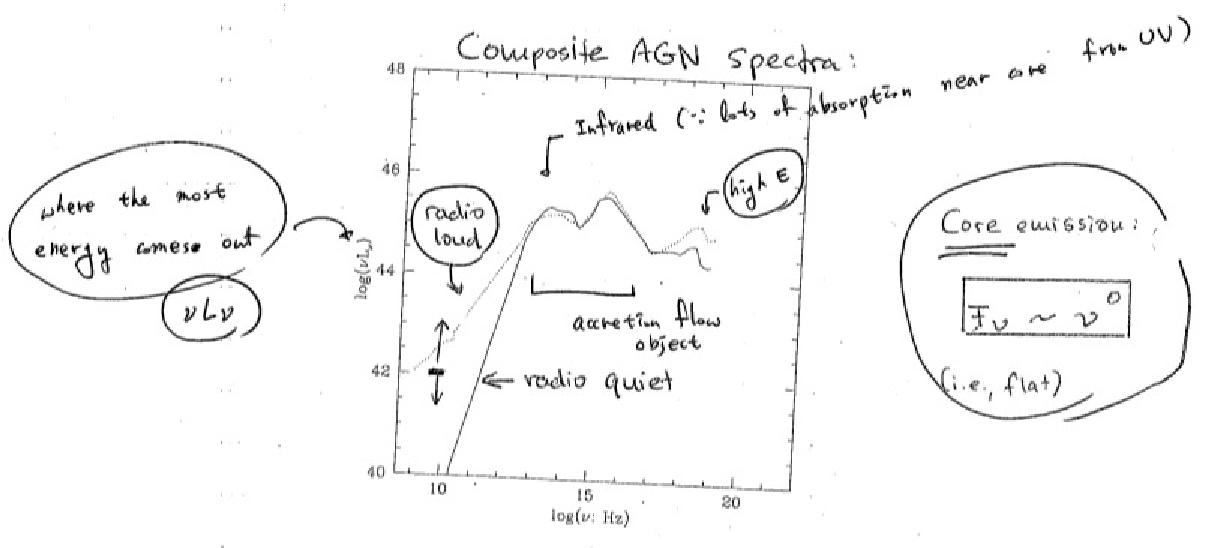
\includegraphics[width=\textwidth]{HighEnergy/note07}
   \caption{Composite AGN Spectra. Dotted line represents radio-loud AGN and solid line represents radio-quiet AGN.}
\label{fig:AGNspectra}
\end{figure}

   $\nu L_{\nu}$ spectrum indicates where the most energy comes out (See fig.(\ref{fig:AGNspectra})).

   ``Radio loud'' AGN: Flat radio spectra from the nuclear region. $F_{\nu} \sim \nu^{0}$

   Radio loudness, 

\begin{equation}
   R = \frac{L_{radio}}{L_{bol}} \simeq \frac{L_{5Ghz}}{L_{B}}
\end{equation}
where $L_{B}$ is luminosity in B-band. We classify AGN as Radio loud, when $R > 2\times 10^{-4}$.

$L_{radio} \sim {\rm few} \times 10^{30}$ to ${\rm few} \times 10^{42}\,\unitpower$

\textbf{BL-Lac objects and ``blazars''}

Some sources are completely dominated by jet emission, \ie, the broad emission lines are hardly seen.

BL-Lacertae-objects and ``blazars''

\begin{figure}[!htbp]
   \centering
   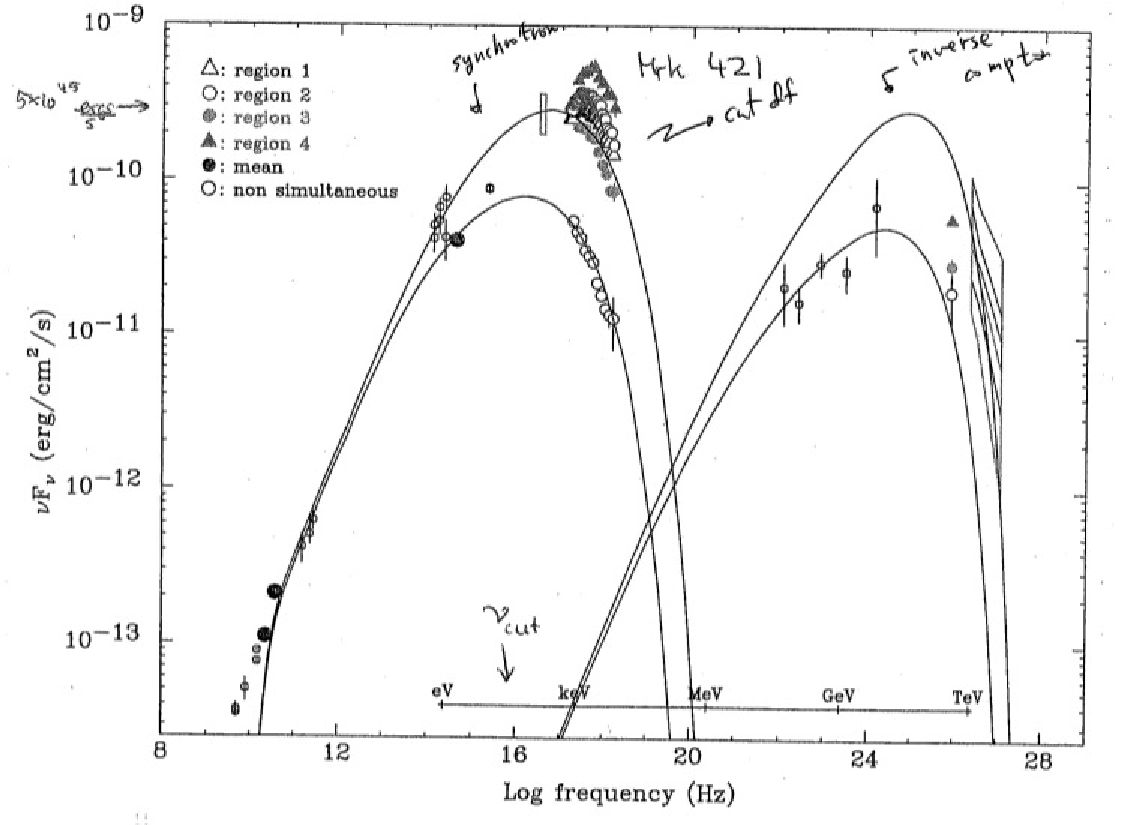
\includegraphics[width=0.7\textwidth]{HighEnergy/note08}
   \caption{Spectrum of BL-Lac object}
\label{fig:BLspectrum}
\end{figure}

These objects, fig.(\ref{fig:BLspectrum}), have pure power-law spectrum up to some cut-off frequency $\nu_{cut}$.
Furthermore, they have X-ray \& $\gamma$-ray spectra of the same shape.

\textbf{Extended emission:}
   \begin{itemize}
      \item Jets show radio spectra with index $\alpha \approx 0.6$, where

\begin{equation}
   F_{\nu} \propto \nu^{-\alpha}
\end{equation}
   cf) core emission: $F_{\nu} \propto \nu^{0}$, \ie flat spectrum

      \item Radio lobes show steeper spectra with $\alpha \approx 1-2$, since optically thin relatively to central region.
   \end{itemize}

\textbf{Polarization:}

Jet emission is almost always polarized. The degree of polarization ranges from a few tenths of a percent to almost 70\%.

We observe strongly polarized power-law (non-thermal) emission across the entire electromagnetic spectrum.

Possible processes:

   \begin{enumerate}[1)]
      \item Synchrotron radiation
      \item Inverse Compton emission
   \end{enumerate}

Answer: Both (Synchrotron at low and inverse compton at high frequencies)

This morphological dichotomy is a fundamental property of radio galaxies.

\end{enumerate}

\subsubsection{Evidence for relativistic motion}

\begin{enumerate}[a)]
   \item Proper motion  (super-luminal motion)
\begin{figure}[!htbp]
   \centering
   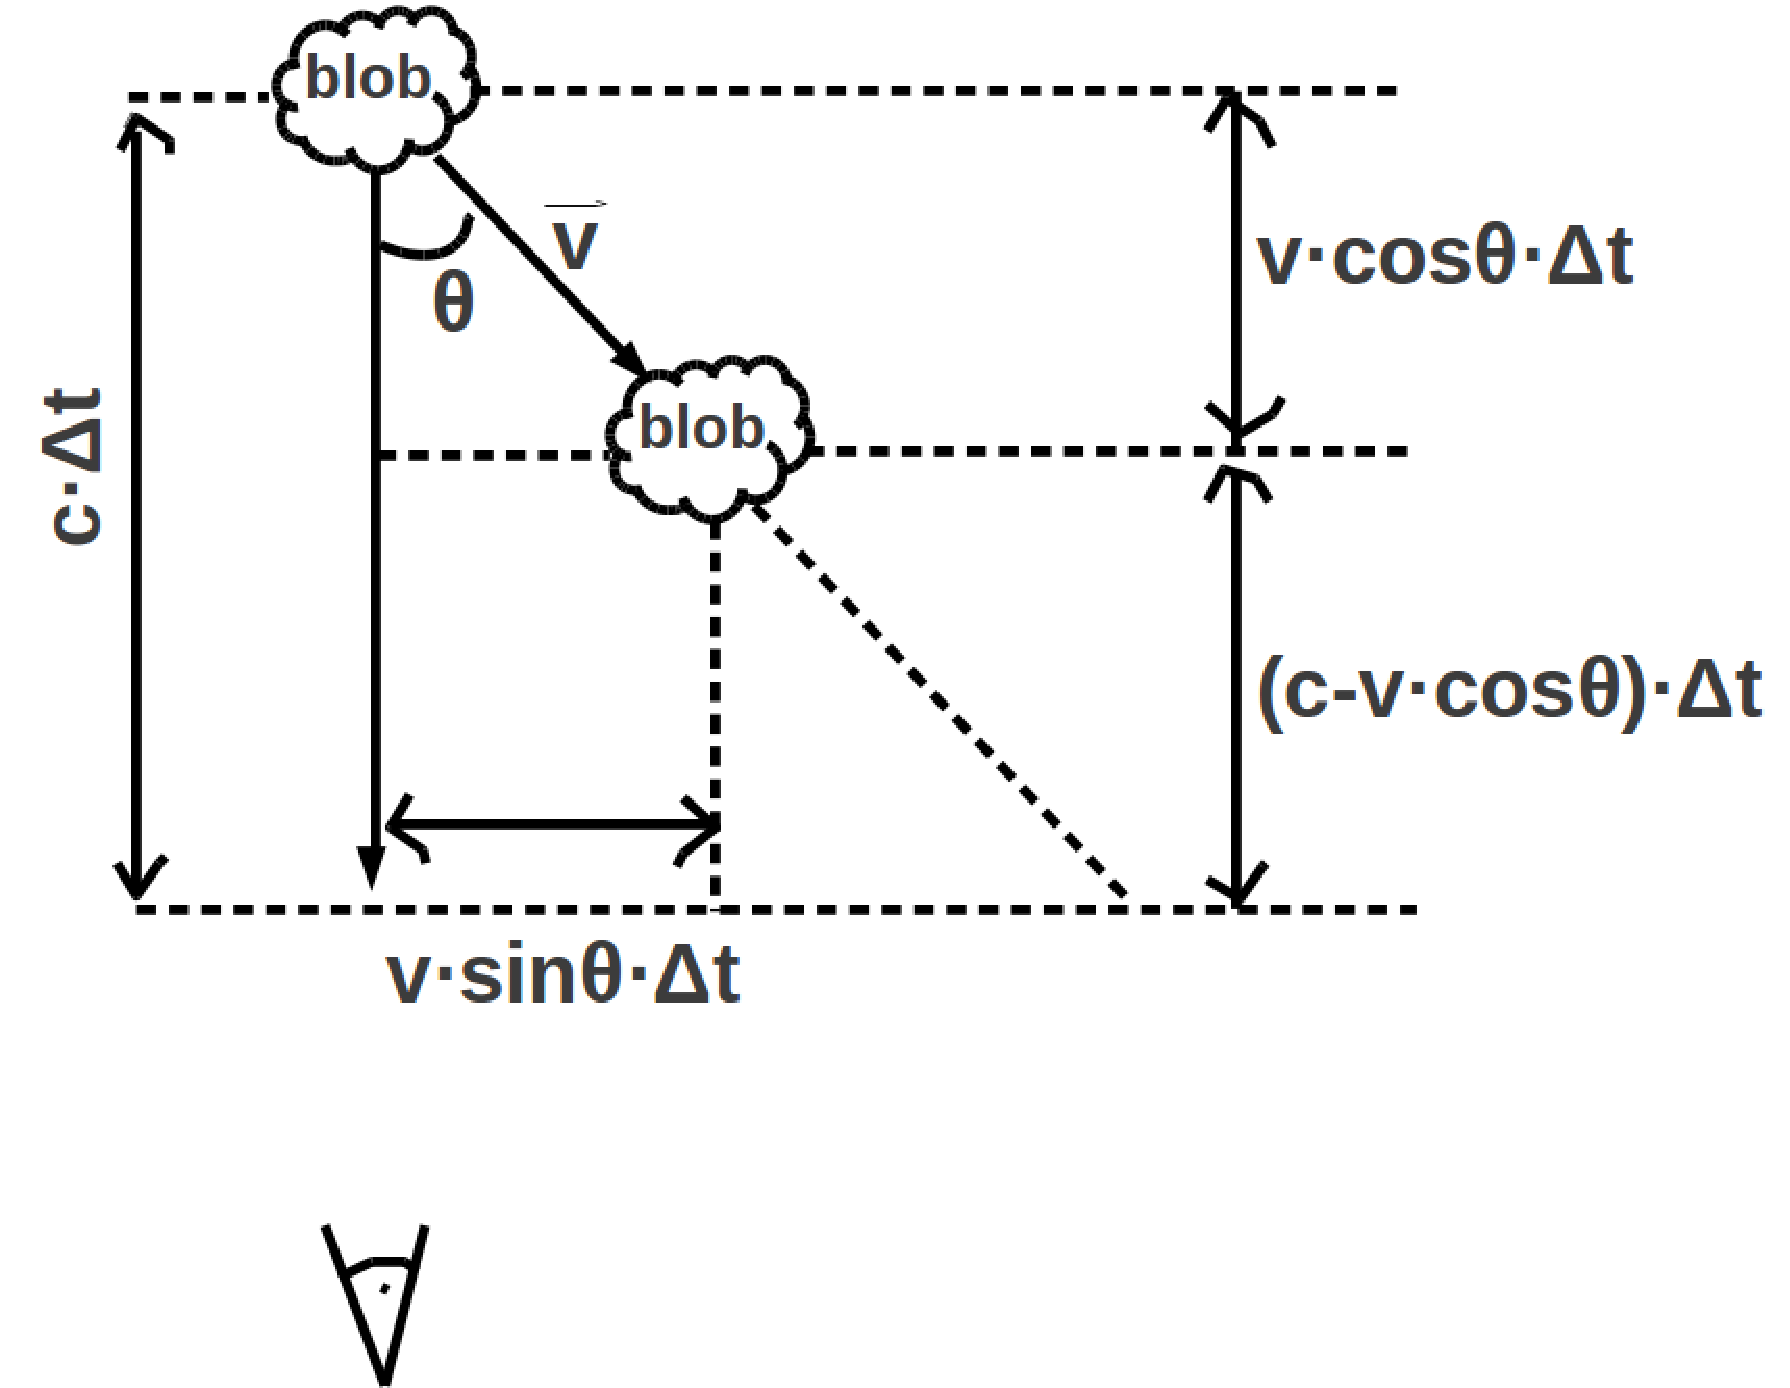
\includegraphics[width=0.7\textwidth]{HighEnergy/superluminal}
   \caption{Super-luminal motion}
\label{fig:superluminal}
\end{figure}

   \begin{enumerate}
      \item perceived distance traveled

\begin{equation}
   \Delta x = v\cdot \sin \theta \cdot \Delta t
\end{equation}
     
      \item perceived time elapsed

\begin{equation}
   \Delta \tau = \frac{\Delta y}{c}  = \frac{(c-v\cdot \cos \theta)\Delta t}{c} = \left( 1-\beta \cos \theta \right)\Delta t 
\end{equation}
   \end{enumerate}

$\Rightarrow$ perceived proper motion:

\begin{empheq}[innerbox=\fbox,
left=\therefore~~]{align}
v_{obs} = \frac{\Delta x}{\Delta \tau} = \frac{v\cdot \sin \theta}{1-\beta \cos \theta}
\end{empheq}
or,
\begin{empheq}[innerbox=\fbox]{align}
\beta_{obs} = \frac{\beta \sin \theta}{1-\beta \cos \theta}
\end{empheq}
Recall $\beta < 1$,
\begin{eqnarray}
   \beta_{obs} = \frac{\beta \sin \theta}{1-\beta(1-\sin^{2} \theta)^{1/2}} \nonumnext
   \Rightarrow ~~ \frac{1}{\beta} = (1-\sin^{2})^{1/2} + \frac{\sin \theta}{\beta_{obs}} > 1 
\end{eqnarray}
\begin{empheq}[innerbox=\fbox,
left=\Rightarrow~~]{align}
\sin \theta < \frac{2 \beta_{obs}}{1+\beta_{obs}} ~~ \textrm{or} ~~ \theta < \frac{2}{\beta_{obs}}~~\textrm{for}~~\beta_{obs} \gg 1
\end{empheq}
Recall
\begin{empheq}[innerbox=\fbox]{align}
\beta \Gamma \ge \beta_{obs}
\end{empheq}
where $\Gamma = \sqrt{1/(1-\beta^{2})}$. Note that $\beta_{obs}$ might not be a physical speed,
\ie, a pattern speed from a moving shock.
Note that Superluminal motion is not a relativistic effect, it is purely a light-travel time effect.
\begin{figure}[!htbp]
   \centering
   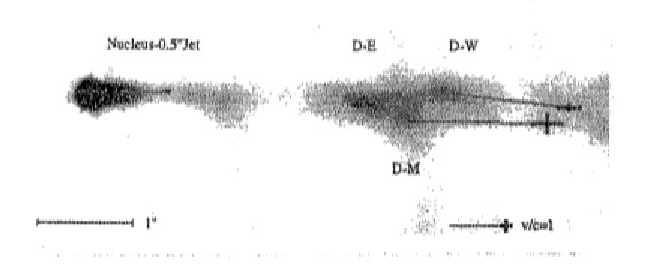
\includegraphics[width=\textwidth]{HighEnergy/note10}
   \caption{M87. $\beta_{obs} \sim 3-5$}
\label{fig:M87}
\end{figure}
Most extreme blazars: $\beta_{obs} \sim 30-50 !$

   \item \textbf{Relativistic Doppler boosting}: relativistic beaming + blue shift

   FRII sources are almost always one-sided. This is easily understood as a consequence of Doppler boosting.

   Assume each source has two equal jets traveling in opposite directions (jet and counter-jet). Each
   emits radiation at a rate $L_{\nu}$ in its own, co-moving frame. Doppler boosting implies that
   the detected luminosity is 

\begin{equation}
   L_{obs} = \delta^{k+\alpha} L_{\nu}
\end{equation}
where $k$ is what kind of object you're looking at, and $\delta$ is the Doppler factor,
\begin{equation}
   \delta = \frac{1}{\Gamma (1-\beta \cos \theta)}
\end{equation}
In case of moving away, $\delta = \frac{1}{\Gamma (1+\beta \cos \theta)}$.
Note that
\begin{empheq}[left=\Rightarrow\empheqlbrace]{align}
   \theta \ll 1~~ &\rightarrow~~ \delta \gg 1 ~~\textrm{for}~ \theta < 1/\Gamma \nonumnext
   \theta \gg 1~~ &\rightarrow~~ \delta \sim 1/\Gamma \ll 1
\end{empheq}
$\alpha$ is the spectral index ($F_{\nu} \propto \nu^{-\alpha}$), and 
\[ \left. \begin{array}{ll}
k=2 & \textrm{(continuous emission)} \\
k=3 & \textrm{(blob-emission)}
\end{array} \right. \]
and $\beta=v/c,~ \Gamma=1/\sqrt{1-\beta^{2}},~\theta$=angle to line-of-sight.
The jet-to-counter-jet brightness ratio is then,
\begin{equation}
   \frac{L_{obs,jet}}{L_{obs,counter-jet}} = \left( \frac{1+\beta \cos \theta}{1-\beta \cos \theta} \right)^{k+\alpha} \equiv l^{k+\alpha}
\end{equation}

Note:
      \subitem 1) $\Gamma$ cancels out ~~~ (convenient)
      \subitem 2) $L$ cancels out ~~~ (distance independence !)
      \subitem 3) $\beta$ and $\theta$ only enter as product $\Rightarrow$ can only measure $\beta \cdot \cos \theta$

\begin{empheq}[innerbox=\fbox]{align}
   \beta\cdot\cos\theta = \frac{l-1}{l+1}
\end{empheq}
Since we know $\beta<1$ and $\cos \theta \le 1$:
\begin{equation}
   \beta \ge \frac{l-1}{l+1} ~~~\textrm{and}~~~ \cos\theta > \frac{l-1}{l+1}
\end{equation}

Example: M87

$~~~~~ L_{obs,jet} \ge 380 \cdot L_{obs,counter-jet}$ \\
$~~~~~ \Rightarrow ~~ l_{obs} \ge 11$ \\
$~~~~~ \Rightarrow ~~ \beta \ge 0.83 ~~~\textrm{and}~~~ \theta < 34^{\circ}$ \\
$~~~~~~ \textrm{where}~ \Gamma \ge 2$ 

   \item Variability
   
   Some radio loud AGN (\eg, blazars) vary on time scales of days and shorter across the entire spectrum. 

   Causality implies a source size limit of 
\begin{equation}
   \Delta r \le c\cdot \Delta t \sim 10^{16} \rm\,cm
\end{equation}
Note: the observed time $\Delta t_{obs}$ is shorter by a factor $\delta^{-1}$ than the co-moving time,
\begin{equation}
   \Delta t_{obs} = \Delta t_{co} / \delta
\end{equation}
The emission is polarized and follows a roughly flat power-law $\Rightarrow$ optically thick synchrotron emission.
For a typical luminosity of $10^{42} \,\unitpower$ at 5 Ghz, the surface brightness of the emission (observed) is
\begin{equation}
   S_{\nu,obs} = \frac{L_{\nu,obs}}{(4\pi)(\pi \Delta r^{2})} = 0.05 \,\rm erg\,cm^{-2}\,s^{-1}Hz^{-1}Sr^{-1}
\end{equation}
which corresponds to a brightness temperature of 
\begin{equation}
   T_{b,obs} = \frac{c^{2}}{2\nu^{2}k} \cdot S_{\nu} \approx 10^{16} K ~~~(\textrm{not reasonable})
\end{equation} 
Recall from synchrotron theory of self-absorbed sources:
\begin{equation}
   S_{\nu} = \frac{j_{\nu}}{\alpha_{\nu}} \propto B^{-1/2} \nu^{5/2}
\end{equation}
where $j_{\nu}$ is emissivity and $\alpha_{\nu}$ is absorption coefficient. Up to some maximum frequency
$\nu_{peak}$, so the bolometric radiation energy density is
\begin{equation}
   u_{rad} \sim \frac{S_{peak}}{c} \propto B^{-1/2} \nu_{peak}^{5/2}
\end{equation}
while the magnetic energy density follows 
\begin{equation}
   u_{B} = \frac{B^2}{8\pi} \propto B^{2}
\end{equation}
Now, recall from synchrotron and inverse Compton theory that losses are proportional to $u_{B}$ and $u_{rad}$,
respectively. If $u_{rad}$ is ever larger than $u_{B}$, Compton losses grow exponentially (instability) and cool
the particle distribution to the point where $u_{rad} \le u_{B}$ again (this is called the ``Compton catastrophe'')

$\Rightarrow$ In synchrotron emitting sources: $u_{B} \ge u_{rad}$

We can re-write this, using $u_{rad} \sim B^{-1/2}\nu_{peak}^{5/2}$:
\begin{eqnarray}
   u_{rad} / u_{B} &<& \rm const \nonumnext
   \Rightarrow B^{-5/2}\, \nu_{peak}^{5/2} &<& \rm const \nonumnext
   B^{-1/2}\, \nu_{peak}^{1/2} &<& \rm const ~~~\equiv~~~ T_{max}
\end{eqnarray}
Plugging the expression for $S_{peak}$ in, this gives
\begin{equation}
   S_{peak} \sim B^{-1/2}\nu_{peak}^{5/2} < T_{max}\nu_{peak}^{2}
\end{equation}
or
\begin{equation}
   {T_{B,peak}} = \frac{S_{peak}c^{2}}{2\,k\,\nu_{peak}^{2}} < T_{max} \approx 10^{12}\,K
\end{equation}
Thus, the brightness temperature of a synchrotron emitting source is limited to 
\begin{equation}
   T_{B} < 10^{12}\, K
\end{equation}

The only way to bring the observed $10^{16} \rm\,K$ in line with this limit is relativistic motion:

   \subitem 1) ~~$\Delta r_{obs} \propto \Delta t_{obs} \propto \Delta t \cdot \frac{1}{\delta} $
   \subitem 2) ~~$\nu_{obs} \propto \nu\cdot \delta$
   \subitem 3) ~~$L_{\nu,obs} \propto L_{\nu}\cdot \delta^{k+\alpha}$

   \subitem $\Rightarrow ~~ T_{obs} \propto \delta^{k+\alpha} \sim \delta^{3}$
   \subitem \textbf{$\Rightarrow ~~\delta \sim 10^{4/3} \sim 20 $}
               
   \item Physical parameters

   Given a physical size and luminosity, we can use synchrotron theory to constrain the physical conditions in the source.

   Recall:

\begin{equation}
   j_{\nu} \approx 10^{-18} \, p\,B^{(p+1)/2}\,\nu_{5GHz}^{-(p-1)/2} \, erg\,cm^{-3}\,s^{-1}Hz^{-1}
\end{equation}
where p is pressure density in relativistic particles ($\united$).

   Example: M87, ``knot A''

   ~~~~ $L_{5Ghz} \approx 5\times10^{29} {\rm\,erg\,s^{-1}Hz^{-1}} \cdot \delta^{-2-\alpha}$

   ~~~~ size: $\Delta r \approx \rm 100 pc$

   ~~~~ $\rightarrow ~~ j_{5Ghz} \approx 4\times10^{-33} \,{\rm erg\,cm^{-3} \,s^{-1} Hz^{-1}} ~~\delta^{-2-\alpha}$ 

   ~~~~ $\rightarrow ~~ p \, B^{1.5} \approx 4\times 10^{-15} \delta^{-2-\alpha}$


   ~~~~ Without a way to measure B directly, we usually proceed to make the (usually poorly justified) assumption of equipartition:

\begin{eqnarray}
   p &\approx& \frac{B^{2}}{8\pi} \\
   \rightarrow p &\approx&  2\times10^{-10} \,erg\,cm^{-3} \delta^{-10/7} \nonumnext
   B &\approx& 100 \, \mu G ~\delta^{-5/7} \nonumber
\end{eqnarray}
We also know that $\Gamma \sim 5$
So roughly,
\begin{empheq}[innerbox=\fbox]{align}
   L_{kin} &\sim \left( 4p+B^{2}/4\pi \right) \pi \Delta r^{2} \Gamma^{2} \beta^{2} c \\ 
           &\sim 3\times 10^{43} \, erg\,s^{-1}
\end{empheq}
(Note: this is just an illustrative example, the numbers are order-of-magnitude accurate only.)

M87 is an FRI source, which is consistent with this kind of power estimate.

Recall from accretion section: $\dot{M}_{\rm Bondi} \sim 0.03 \,\unitmfluxsol$

\begin{empheq}[innerbox=\fbox]{align}
   L_{\rm Bondi} \sim 2\times 10^{43}\, \unitpower
\end{empheq}

\end{enumerate}

\textcolor{red}{compton scattering 
inverse compton scattering}

\bigskip
\subsection{Binary System}

\subsubsection{Kepler's Law}

\noi 1. The orbit of every planet is an ellipse with the sun at one of two foci.
\begin{equation}
   r = \frac{p}{1+\epsilon \cos \theta} \nonumber
\end{equation}
\noindent where p=b$^{2}$/2 (semi-latus rectum), $\epsilon = \sqrt{1-(b/a)^{2}}$ (eccentricity).

\noi 2. A line joining a planet and the sun sweeps out equal area during equal intervals of time.
\begin{equation}
   \frac{d}{dt}\left( \frac{1}{2} r^{2}\theta \right) = 0. \nonumber
\end{equation}

\noi 3. The square of the orbital period of a planet is directly proportional to the cube of the 
semi-major axis of its orbit.
\begin{equation}
   T^{2} = \frac{4\pi^{2}a^{3}}{\textrm{GM}}. \nonumber
\end{equation}

\noi 4. Center of Mass
\begin{equation}
    r_{1}M_{1} = r_{2}M_{2}
\end{equation}
Therefore,
\begin{equation}
    r_{1} = \frac{M_{2}}{M_{1}+M_{2}}\,r
\end{equation}
or,
\begin{equation}
    r_{2} = \frac{M_{1}}{M_{1}+M_{2}}\,r
\end{equation}
where $r = r_{1}+r_{2}$. In this context, the Kepler's law can be expressed as,
\begin{equation}
    \omega^{2} = \frac{G\left( M_{1}+M_{2} \right)}{a^{3}},
\end{equation}
where $\omega = 2\,\pi/T$.

\noi 5. Inclination angle: $i$
If the normal vector of the orbital plane is inclined to the line of sight by an angle $i$, the 
Doppler velocity amplitudes we measure will be 
\begin{equation}
    |v_{1obs}| = |v_{1}|\sin{i}, ~~~ |v_{2obs}| = |v_{2}|\sin{i}.
\end{equation}
Then,
\begin{equation}
    \frac{M_{2}^{3}}{(M_{1}+M_{2})^{2}}\sin^{3}{i} = \frac{\tau |v_{1obs}|^{3}}{2\pi\,G},
\end{equation}
where $\tau = 2\pi\,r_{1}/|v_{1}| = 2\pi\,r_{2}/|v_{2}|$. The detailed derivation is in \cite{Maoz}.

\subsubsection{Tidal force}
\begin{equation}
   dF_{\textrm{Tidal}} = \frac{2 G M m dr}{r^{3}} \nonumber
\end{equation}


   \chapter{Cosmology}


\section{Hubble law}
The relative velocity $v$ between two galaxies that are separated by a large distance r is given by the 
Hubble law:
\begin{equation}
   v = H_{0}\,r,
\end{equation}
where $H_{0}$ is the {\bf Hubble constant}:
\begin{equation}\label{eq:hubbleconst}
    H_{0} = (72 \pm 8)\,{\rm km\,s^{-1}\,Mpc^{-1}}.
\end{equation}



   \chapter{Particle Physics}

Leptons: the lightest particles are spin-1/2 fermions that do not experience the strong nuclear force, but observe Pauli's exclusion principle.

\begin{table}[ht] 
  \centering  
  \begin{tabular}{c c c} 
  \hline \hline  
%head  
     & charged & neutrino \\ 
  \hline 
%data  
    electronic & $e^{-}     ~(0.511 Mev) \footnotemark $ & $\nu_{e}$ \\
    muonic     & $\mu^{-}$  ~(105.6 MeV) & $\nu_{\mu}$ \\
    tauonic    & $\tau^{-}$ ~(1777 MeV) & $\nu_{\tau}$ \\
  \hline 
  \end{tabular} 
\end{table}
\footnotetext{the rest mass energy}

$e^{-}$ are stable, the most common and least mass charged lepton in the universe.

Hadrons: 
\begin{itemize}
   \item Baryons: fermions that are strongly interacting. \\
         Greek means ``heavy particles''. \\ 
         The lightest and most familiar baryons are the proton and the neutron.
   \item Mesons: ``messenger'' particles made of an even number of quarks and antiquark. \\
         They are bosons. \\
         $\sigma^{-},\omega^{-},\rho-\textrm{mesons, Pions}(\pi)$ and kaons $(K^{+},K^{0},\bar{K}^{0},K^{-})$.
\end{itemize}



   \chapter{Mathematical physics}

\section{Mathematical physics}

\subsection{Moment of Inertia}

Moment of inertia is the name given to rotational inertia, the rotational analog of mass for
linear motion.  It appears in the relationships for the dynamics of rotational motion. The
moment of inertia must be specified with respect to a chosen axis of rotation. For a point
mass, the moment of inertia is just the mass times the square of perpendicular distance to
the rotation axis, $I=m\,r^{2}$. That point mass relationship becomes the basis for all other
moment of inertia since any object can be built up from a collection of point masses. For the
extended source, we have to integrate through the volume,

\begin{equation}
   I = \int dI = \int^{M}_{0}r^{2}dm
\end{equation}

\subsubsection{sphere}

To derive the moment of inertia of a solid sphere of uniform density and radius R,
\begin{equation}
   dI = r^{2}_{\perp} dm = r^{2}_{\perp}\rho\,dV
\end{equation}
where $r_{\perp}$ is the perpendicular distance to a point at $\vec{r}$ from the axis of rotation.
Therefore, $r_{\perp}= |\vec{r}|\,\sin{\theta}$. Integrating over the volume,
\begin{eqnarray}
   I &=& \int \int \int_{V} \rho\,r^{2}_{\perp}\,dV = \rho \int^{2\pi}_{0}\int^{\pi}_{0}\int^{R}_{0} \left( r\,\sin{\theta} \right)^{2}\,r^{2}\,\sin{\theta}drd\theta d\phi \nonumnext
     &=& 2\pi\rho \int^{\pi}_{0} \sin^{3}{\theta}d\theta \int^{R}_{0}r^{4}dr ~~~~~~~~~ \leftarrow \textrm{substituting } u=\cos{\theta} \nonumnext
     &=& 2\pi\rho \frac{R^{5}}{5}\int^{1}_{-1} \left( 1 - u^{2} \right) du = \frac{4}{3}\pi R^{3}\rho\left( \frac{2}{5} R^{2}\right) \nonumnext
     &=& \frac{2}{5}M\,R^{2}
\end{eqnarray}
where $M$ is the total mass of the sphere.


\bigskip
\subsection{Potential of Uniform Sphere}\label{subsec:potunisp}
To be updated
\begin{equation}
    U = -\frac{3}{5} \frac{G\,M}{R}
\end{equation}

\bigskip
\subsection{Fourier decomposition}



%   \include{Numerical/numerical}
   \chapter{Instrument}

\section{Optical}
\begin{itemize}
    \item Angular resolution
\begin{equation}
    \theta = 1.22\,\frac{\lambda}{D},
\end{equation}
where a plane wave of wavelength $\lambda$ passing through a circular aperture of diameter $D$. 
\end{itemize}
\section{Radio}
\section{X-ray}
\section{Infrared}



   \appendix
   \chapter{Appendix}

\section{Astrophysical Constants}

\newcommand{\va}{\boldsymbol{a}}
\newcommand{\vb}{\boldsymbol{b}}
\newcommand{\vc}{\boldsymbol{c}}
\newcommand{\vd}{\boldsymbol{d}}

\newcommand{\vA}{\boldsymbol{A}}
\newcommand{\vB}{\boldsymbol{B}}
\newcommand{\vn}{\boldsymbol{n}}
\newcommand{\vl}{\boldsymbol{l}}

\newcommand{\ux}{\boldsymbol{\hat{x}}}
\newcommand{\uy}{\boldsymbol{\hat{y}}}
\newcommand{\uz}{\boldsymbol{\hat{z}}}
\newcommand{\urh}{\boldsymbol{\hat{\rho}}}
\newcommand{\up}{\boldsymbol{\hat{\phi}}}
\newcommand{\urr}{\boldsymbol{\hat{r}}}
\newcommand{\ut}{\boldsymbol{\hat{\theta}}}
\newcommand{\st}{\sin{\theta}}
\newcommand{\boldT}{\boldsymbol{T}}

\begin{deluxetable}{ll | ll}
%\tabletypesize{\footnotesize}
\tabletypesize{\scriptsize}
\tablecolumns{4}
\tablewidth{0pt}
\tablehead{\multicolumn{4}{c}{\bf{Physical and Astrophysical constants}} \\
           \colhead{Constant} & \colhead{CGS unit} & \colhead{Constant} & \colhead{CGS unit}}
\startdata
c$_{0}$ (speed of light in vacuum) & $2.99792458\times10^{10}$ cm s$^{-1}$ &
h (Plank constant) & $6.6260755\times10^{-27}$ erg s \\
e (electron charge) & $4.80320680\times10^{-10}$ esu &
$\alpha$ (fine structure constant) & 1/137.03598951 \\
m$_{e}$ (electron mass) & $9.1093897\times10^{-28}$ g &
r$_{e}$ (classical electron radius) & $2.81794092\times10^{-13}$ cm \\ 
m$_{p}$ (proton mass) & $1.672631\times10^{-24}$ g &
Bohr radius & $0.529177249\times10^{-8}$ cm \\
m$_{n}$ (neutron mass) & $1.6749286\times10^{-24}$ g &
G (gravitational const) & $6.67259\times10^{-8}$ cm$^3$g$^{-1}$s$^{-2}$ \\
m$_{d}$ (deuteron mass) & $3.34358602\times10^{-24}$ g &
G'(gravitational const) \tablenotemark{**} & $4.298$ M$_{\odot}^{-1}$pc$^{2}$km$^{2}$s$^{-2}$kpc$^{-1}$ \\
u (unified atomic mass) & $1.6605402\times10^{-24}$ g &
N$_A$ (Abogadro const) & $6.0221367\times10^{23}$ mol$^{-1}$ \\
k (Boltzmann constant) & $1.380658\times10^{-16}$ erg K$^{-1}$ &
b (Wien disp. law const) & $0.2897756$ cm K \\
$\sigma_{\textrm{SB}}$ (Stefan-Boltzman const) & $5.67\times10^{-5}$ erg s$^{-1}$cm$^{-2}$K$^{-4}$ &
AU (astronomical unit) & $1.4959787066\times10^{13}$ cm \\
Jy (Jansky) & $10^{-23}$ erg s$^{-1}$ cm$^{-2}$ Hz$^{-1}$ &
pc (parsec) & $3.0856775807\times10^{18}$ cm \\
M$_{\odot}$ (Solar mass) & $1.98892\times10^{33}$ g &
ly (light year) & $0.9461\times10^{18}$ cm \\
M$_{\textrm{Earth}}$ (Earth mass) & $5.97370\times10^{27}$ g &
ev (electron volt) & $1.602\times10^{-12}$ erg \\
M$_{\textrm{Moon}}$ (Moon mass) & $7.348\times10^{25}$ g &
Plank Mass & $2.17671\times10^{-5}$ g \\
L$_{\odot}$ (Solar luminosity) & $3.846\times10^{33}$ erg s$^{-1}$ &
Plank length & $1.61605\times10^{-33}$ cm \\
R$_{\odot}$ (Solar radius) & $6.955\times10^{10}$ cm &
Plank time & $5.39056\times10^{-44}$ s \\
$\sigma_{\textrm{T}}$ (Thompson Cross section) & $6.65246154\times10^{-25}$ cm$^{2}$ &
J (Joule) & $10^7$ erg \\
$\epsilon_{0}$ (permittivity of vacuum) \tablenotemark{*} & $8.854\times10^{-12}$ C$^{2}$m$^{-2}$N$^{-1}$ &
N (Newton) & $10^5$ dyne \\
$\mu_{0}$ (permeability of vacuum) \tablenotemark{*} & $4\pi\times10^{-7}$ H m$^{-1}$ &
yr (year) & $3.155693\times10^{7}$ s \\
Tesla & $10^4$ Gauss &
\enddata
\tablenotetext{*}{ SI unit ; In cgs unit, $\epsilon_{0}$ and $\mu_{0}$ are unity. }
\tablenotetext{**}{ special unit }
\end{deluxetable}

\clearpage

\section{Vector Identity}
~~~~
\bigskip

\begin{eqnarray}
\va \cdot \left( \vb \times \vc \right) &=& 
    \vb \cdot \left( \vc \times \va \right) = \vc \cdot \left( \va \times \vb \right) \nonumnext
\va \times \left( \vb \times \vc \right) &=& 
\left( \va \cdot \vc \right)\vb - \left( \va \cdot \vb \right)\vc \nonumber \nonumnext 
\left( \va \times \vb \right) \cdot \left( \vc \times \vd \right) &=& 
\left( \va \cdot \vc \right) \left( \vb \cdot \vd \right) - \left( \va \cdot \vd \right) \left( \vb \cdot \vc \right) \nonumnext
\nabla \times \nabla \psi &=& 0 \nonumnext
\nabla \cdot \left( \nabla \times \va \right) &=& 0 \nonumnext 
\nabla \times \left( \nabla \times \va \right) &=&
\nabla \left( \nabla \cdot \va \right) - \nabla^{2} \va \nonumnext
\nabla \cdot \left( \psi \va \right) &=& \va \cdot \nabla \psi + \psi \nabla \cdot \va \nonumnext
\nabla \times \left( \psi \va \right) &=& \nabla \psi \times \va + \psi \nabla \times \va \nonumnext
\nabla\left( \va \cdot \vb \right) &=& 
\left( \va \cdot \nabla \right)\vb + \left( \vb \cdot \nabla \right)\va
+ \va \times \left( \nabla \times \vb \right) + \vb \times \left( \nabla \times \va \right) \nonumnext
\nabla \cdot \left( \va \times \vb \right) &=& 
\vb \cdot \left( \nabla \times \va \right) - \va \cdot \left( \nabla \times \vb \right) \nonumnext
\nabla\times\left( \va \times \vb \right) &=&
\va\left( \nabla \cdot \vb \right) - \vb\left( \nabla \cdot \va \right)
+\left( \vb \cdot \nabla \right)\va - \left( \va \cdot \nabla \right)\vb  \nonumber
\end{eqnarray}

\clearpage

\section{Vector Calculus}
~~~~
\bigskip

\begin{eqnarray}
\int_{V} \nabla \cdot \vA ~d^{3}x &=& \int_{S} \vA \cdot \vn ~da 
\textrm{~~~~~~~~~~~~~~~~~~~~~~~~~(Divergence Theorem)} \nonumnext
\int_{V} \nabla \psi d^{3}x &=& \int_{S} \psi \vn ~da  \nonumnext
\int_{V} \nabla \times \vA ~d^{3}x &=& \int_{S} \vn \times \vA ~da \nonumnext 
\int_{V} \left( \phi \nabla^{2}\psi + \nabla\phi \cdot \nabla\psi \right) d^{3}x &=&
\int_{S} \phi \vn\cdot\nabla\psi da
\textrm{~~~~~~~~~~~~~~~~~~~~~~(Green's first identity)} \nonumnext
\int_{V} \left( \phi \nabla^{2}\psi - \psi\nabla^{2}\phi \right) d^{3}x &=&
\int_{S} \left( \phi\nabla\psi - \psi\nabla\phi \right) \cdot \vn ~da 
\textrm{~~~~~~~~~(Green's theorem)} \nonumnext
\int_{S} \left( \nabla \times \vA \right) \cdot \vn ~da &=& \oint_{C} \vA \cdot d\vl 
\textrm{~~~~~~~~~~~~~~~~~~~~~~~~~~~~~(Stokes's theorem)} \nonumnext
\int_{S} \vn \times \nabla \psi da &=& \oint_{C} \psi d\vl \nonumber
\end{eqnarray}

\clearpage

\section{Coordinate System}

~~~~
\bigskip
\subsection{Cartesian (x,y,z)}

\begin{eqnarray}
\nabla \psi &=& \frac{\partial\psi}{\partial x}\ux + \frac{\partial\psi}{\partial y}\uy + \frac{\partial\psi}{\partial z}\uz \nonumnext
\nabla \cdot \vA &=& \frac{\partial A_{x}}{\partial x} + \frac{\partial A_{y}}{\partial y} + \frac{\partial A_{z}}{\partial z} \nonumnext
\nabla \times \vA &=& \left( \frac{\partial A_{z}}{\partial y} - \frac{\partial A_{y}}{\partial z} \right)\ux
                    + \left( \frac{\partial A_{x}}{\partial z} - \frac{\partial A_{z}}{\partial x} \right)\uy
                    + \left( \frac{\partial A_{y}}{\partial x} - \frac{\partial A_{x}}{\partial y} \right)\uz \nonumnext
(\vA \cdot \nabla)\, \vB &=& \left( A_{x}\frac{\partial B_{x}}{\partial x} 
                                + A_{y}\frac{\partial B_{x}}{\partial y} 
                                + A_{z}\frac{\partial B_{x}}{\partial z} \right) \ux 
                          +\left( A_{x}\frac{\partial B_{y}}{\partial x} 
                                + A_{y}\frac{\partial B_{y}}{\partial y} 
                                + A_{z}\frac{\partial B_{y}}{\partial z} \right) \uy \nonumnext
                        &&+\left( A_{x}\frac{\partial B_{z}}{\partial x} 
                                + A_{y}\frac{\partial B_{z}}{\partial y} 
                                + A_{z}\frac{\partial B_{z}}{\partial z} \right) \uz \nonumnext
\nabla^{2}\psi &=& \frac{\partial^{2} \psi}{\partial x^{2}} + \frac{\partial^{2} \psi}{\partial y^{2}} + \frac{\partial^{2} \psi}{\partial z^{2}} \nonumnext
\nabla \cdot \boldT_{i,j} &=& 
     \left( \frac{\partial T_{xx}}{\partial x} 
     + \frac{\partial T_{yx}}{\partial y} + \frac{\partial T_{zx}}{\partial z} \right) \ux 
    +\left( \frac{\partial T_{xy}}{\partial x} 
     + \frac{\partial T_{yy}}{\partial y} + \frac{\partial T_{zy}}{\partial z} \right) \uy \nonumnext
    &&+\left( \frac{\partial T_{xz}}{\partial x} 
     + \frac{\partial T_{yz}}{\partial y} + \frac{\partial T_{zz}}{\partial z} \right) \uz \nonumber
\end{eqnarray}

%\begin{center}
%\line(1,0){400}
%\end{center}

~~~~
\bigskip
\subsection{Cylindrical ($\rho$,$\phi$,z)}

\begin{eqnarray}
\nabla \psi &=& \frac{\partial\psi}{\partial \rho}\urh + \frac{1}{\rho}\frac{\partial\psi}{\partial \phi}\up 
              + \frac{\partial\psi}{\partial z}\uz \nonumnext
\nabla \cdot \vA &=& \frac{1}{\rho}\frac{\partial}{\partial \rho}\left( {\rho A_{\rho}} \right) 
                   + \frac{1}{\rho}\frac{\partial A_{\phi}}{\partial \phi} + \frac{\partial A_{z}}{\partial z} \nonumnext
\nabla \times \vA &=& \left( \frac{1}{\rho}\frac{\partial A_{z}}{\partial \phi} - \frac{\partial A_{\phi}}{\partial z} \right)\urh
                    + \left( \frac{\partial A_{\rho}}{\partial z} - \frac{\partial A_{z}}{\partial \rho} \right)\up
                    + \frac{1}{\rho}\left( \frac{\partial}{\partial \rho}\left( \rho A_{\phi} \right) 
                      - \frac{\partial A_{\rho}}{\partial \phi} \right)\uz \nonumnext
(\vA \cdot \nabla)\, \vB &=& \left( A_{\rho}\frac{\partial B_{\rho}}{\partial \rho} 
                                + \frac{A_{\phi}}{\rho}\frac{\partial B_{\rho}}{\partial \phi} 
                                + A_{z}\frac{\partial B_{\rho}}{\partial z} 
                                - \frac{A_{\phi}B_{\phi}}{\rho} \right) \urh   \nonumnext
                          &&+\left( A_{\rho}\frac{\partial B_{\phi}}{\partial \rho} 
                                + \frac{A_{\phi}}{\rho}\frac{\partial B_{\phi}}{\partial \phi} 
                                + A_{z}\frac{\partial B_{\phi}}{\partial z} 
                                + \frac{A_{\phi}B_{\rho}}{\rho} \right) \up  \nonumnext
                          &&+\left( A_{\rho}\frac{\partial B_{z}}{\partial \rho} 
                                + \frac{A_{\phi}}{\rho}\frac{\partial B_{z}}{\partial \phi} 
                                + A_{z}\frac{\partial B_{z}}{\partial z} \right) \uz \nonumnext
\nabla^{2}\psi &=& \frac{1}{\rho}\frac{\partial}{\partial \rho} \left( \rho \frac{\partial \psi}{\partial \rho} \right) 
                 + \frac{1}{\rho^{2}}\frac{\partial^{2} \psi}{\partial \phi^{2}} + \frac{\partial^{2} \psi}{\partial z^{2}} \nonumnext
\nabla \cdot \boldT_{i,j} &=& 
     \left\{ \frac{1}{\rho} \frac{\partial}{\partial \rho} (\rho\,T_{\rho z}) 
     + \frac{1}{\rho} \frac{\partial T_{\phi z}}{\partial \phi} + \frac{\partial T_{zz}}{\partial z}   \right\} \urh \nonumnext
    &&+\left\{ \frac{1}{\rho} \frac{\partial}{\partial \rho} (\rho\,T_{\rho \rho}) 
     + \frac{1}{\rho} \frac{\partial T_{\phi\rho}}{\partial \phi} + \frac{\partial T_{z \rho}}{\partial z} 
     - \frac{T_{\phi\phi}}{\rho} \right\} \up \nonumnext
    &&+\left\{ \frac{\partial T_{\rho \phi}}{\partial \rho} 
     + \frac{1}{\rho} \frac{\partial T_{\phi \phi}}{\partial \phi} + \frac{\partial T_{z\phi}}{\partial z} 
     + \frac{T_{\phi\rho} + T_{\rho\phi}}{\rho}  \right\} \uz \nonumber
\end{eqnarray}

%\begin{center}
%\line(1,0){400}
%\end{center}

~~~~
\bigskip
\subsection{Spherical (r,$\theta$,$\phi$)}

\begin{eqnarray}
\nabla \psi &=& \frac{\partial \psi}{\partial r}\urr + \frac{1}{r}\frac{\partial\psi}{\partial \theta}\ut 
              + \frac{1}{r \st}\frac{\partial\psi}{\partial \phi}\up \nonumnext
\nabla \cdot \vA &=& \frac{1}{r^{2}}\frac{\partial}{\partial r}\left( r^{2} A_{r} \right) 
                   + \frac{1}{r \st}\frac{\partial}{\partial \theta}\left( \st A_{\theta} \right) 
                   + \frac{1}{r \st}\frac{\partial A_{\phi}}{\partial \phi} \nonumnext
\nabla \times \vA &=& \frac{1}{r \st}\left( \frac{\partial}{\partial \theta}\left( \st A_{\phi} \right) 
                      - \frac{\partial A_{\theta}}{\partial \phi} \right)\urr
                    + \left( \frac{1}{r \st}\frac{\partial A_{r}}{\partial \phi} 
                      - \frac{1}{r}\frac{\partial}{\partial r}\left( r A_{\phi} \right) \right)\ut \nonumnext
                  &&+ \frac{1}{r}\left( \frac{\partial}{\partial r}\left( r A_{\theta} \right)  
                      - \frac{\partial A_{r}}{\partial \theta} \right)\up \nonumnext
(\vA \cdot \nabla)\, \vB &=& \left( A_{r}\frac{\partial B_{r}}{\partial r} 
                                + \frac{A_{\theta}}{r}\frac{\partial B_{r}}{\partial \theta} 
                                + \frac{A_{\phi}}{r\,\sin{\theta}}\frac{\partial B_{r}}{\partial \phi} 
                                - \frac{A_{\theta}B_{\theta}+A_{\phi}B_{\phi}}{r} \right) \urr \nonumnext
                          &&+\left( A_{r}\frac{\partial B_{\theta}}{\partial r} 
                                + \frac{A_{\theta}}{r}\frac{\partial B_{\theta}}{\partial \theta} 
                                + \frac{A_{\phi}}{r\,\sin{\theta}}\frac{\partial B_{\theta}}{\partial \phi} 
                                + \frac{A_{\theta}B_{r} - A_{\phi}B_{\phi}\,\cot{\theta}}{r} \right) \ut \nonumnext
                          &&+\left( A_{r}\frac{\partial B_{\phi}}{\partial r} 
                                + \frac{A_{\theta}}{r}\frac{\partial B_{\phi}}{\partial \theta} 
                                + \frac{A_{\phi}}{r\,\sin{\theta}}\frac{\partial B_{\phi}}{\partial \phi} 
                                + \frac{A_{\phi}B_{r} + A_{\phi}B_{\theta}\,\cot{\theta}}{r} \right) \up \nonumnext
\nabla^{2}\psi &=& \frac{1}{r^{2}}\frac{\partial}{\partial r}\left( r^{2} \frac{\partial \psi}{\partial r} \right) 
                 + \frac{1}{r^{2} \st}\frac{\partial}{\partial \theta}\left( \st \frac{\partial \psi}{\partial \theta} \right) 
                 + \frac{1}{r^{2} \sin^{2}\theta}\frac{\partial^{2} \psi}{\partial \phi^{2}} \nonumnext
&& \textrm{Note that}~\frac{1}{r^{2}}\frac{\partial}{\partial r}\left( r^{2}\frac{\partial \psi}{\partial r} \right) \equiv
                      \frac{1}{r}\frac{\partial^{2}}{\partial r^{2}}\left( r \psi \right) \nonumnext
    \nabla \cdot \boldT_{i,j} &=& 
    \left\{ \frac{\partial T_{rr}}{\partial r} + \frac{1}{r}\frac{\partial T_{r\theta}}{\partial \theta} 
    + \frac{1}{r\st}\frac{\partial T_{r\phi}}{\partial \phi} 
    + \frac{2\,T_{rr}+\cot{\theta}\,T_{r\theta}-T_{\theta\theta}-T_{\phi\phi}}{r}  \right\}\,\urr \nonumnext 
    &&+ \left\{ \frac{\partial T_{\theta r}}{\partial r} + \frac{1}{r}\frac{\partial T_{\theta\theta}}{\partial \theta} 
    + \frac{1}{r\st}\frac{\partial T_{\theta\phi}}{\partial \phi} 
    + \frac{T_{r\theta}+2T_{\theta r}+\cot{\theta}(T_{\theta\theta}-T_{\phi\phi})}{r}  \right\}\,\ut  \nonumnext
    &&+ \left\{ \frac{\partial T_{\phi r}}{\partial r} + \frac{1}{r}\frac{\partial T_{\phi\theta}}{\partial \theta} 
    + \frac{1}{r\st}\frac{\partial T_{\phi\phi}}{\partial \phi} 
    + \frac{T_{r\phi}+2T_{\phi r}+\cot{\theta}(T_{\theta\phi}+T_{\phi\theta})}{r}  \right\}\,\up.  \nonumber 
\end{eqnarray}


   \section{Theoretical \& Observational Tools}
to be described
\subsection{Codes}
to be described
\subsubsection{Particle}
\subsubsection{Grid}
\subsubsection{Hybrid}
\textcolor{red}{FLASH, ZEUS, ATHENA, GASOLIN, GADGET, GIZMO, CMHOG, AREPO}

\bigskip
\clearpage

%\bibliographystyle{apj}
%\bibliography{citations}


\backmatter

%\addcontentsline{toc}{chapter}{References}
%\bibliographystyle{plain}
%\bibliography{refs}

\bibliographystyle{apj}
\bibliography{citations}

\end{document}
